\documentclass[aspectratio=169,10pt]{beamer}
% Estilo de la presentación del TP5

\usepackage[T1]{fontenc}
\usepackage[utf8]{inputenc}
\usepackage[spanish,es-noshorthands,es-nodecimaldot]{babel}
\spanishplainpercent

\usepackage{lmodern}
\usefonttheme{professionalfonts}
\usepackage{mathptmx}
\usepackage{amsmath,amssymb}
\DeclareSymbolFont{symbols}{OMS}{cmsy}{m}{n}
\SetSymbolFont{symbols}{bold}{OMS}{cmsy}{b}{n}
\DeclareSymbolFontAlphabet{\mathcal}{symbols}

\usepackage{graphicx}
\usepackage{tikz}
\usepackage{media9}
\usepackage{algpseudocode}
\algrenewcommand\algorithmicrequire{\textbf{Entrada:}}
\algrenewcommand\algorithmicensure{\textbf{Salida:}}
\newcommand{\acc}{a}   % a(r,v) = (-k r - \gamma v)/m

\usetikzlibrary{arrows.meta,positioning}
\graphicspath{{images/}}


\usetheme{Warsaw}
\setbeamertemplate{navigation symbols}{}
\definecolor{acento}{rgb}{0.2,0.2,0.7}
\definecolor{dlat}{HTML}{DB2B2B}   % mismos colores que D_LAT_COLOR / D_ACT_COLOR en scripts/lib/plot_style.py
\definecolor{dact}{HTML}{6E00B7}
\newcommand{\dlat}{\textcolor{dlat}{d_{\mathrm{lat}}}}   % los dos parámetros, siempre en su color (modo matemático)
\newcommand{\dact}{\textcolor{dact}{d_{\mathrm{act}}}}

% Barra de navegación: una columna por sección, un punto por diapositiva.
\useoutertheme[subsection=false]{miniframes}

% Sin esto las diapositivas salen sin numerar.
\setbeamertemplate{page number in head/foot}[framenumber]

% Separador con el título de la sección, sin numerar.
\AtBeginSection[]{%
  \begin{frame}[plain,noframenumbering]
    \vfill\centering\usebeamercolor[fg]{structure}%
    {\Huge\bfseries\insertsectionhead}\vfill
  \end{frame}%
}


\newcommand{\vv}[1]{\mathbf{#1}}
\newcommand{\ten}[1]{\times 10^{#1}}
\newcommand{\uni}[1]{\,\mathrm{#1}}
\newcommand{\va}{v_{a}}

\newcommand{\siimagen}[3]{%
  \IfFileExists{images/#1}{#2}{#3}%
}

\newcommand{\figura}[2][\linewidth]{%
  \siimagen{#2}%
    {\makebox[\linewidth][c]{\includegraphics[width=#1,height=0.74\textheight,keepaspectratio]{#2}}}%
    {\makebox[\linewidth][c]{\framebox[#1][c]{\rule{0pt}{5cm}\textit{falta la figura}}}}%
}


\newenvironment{cols}{\begin{columns}[c]}{\end{columns}}

\newenvironment{resultado}[1][Resultado]{%
  \begin{beamercolorbox}[wd=\linewidth,sep=6pt,rounded=true]{block body alerted}%
  \footnotesize\textbf{#1}\par\vspace{2pt}%
  \begin{itemize}\setlength{\itemsep}{1pt}%
}{%
  \end{itemize}\end{beamercolorbox}%
}

\newenvironment{parametros}[1][Parámetros]{%
  \begin{beamercolorbox}[wd=\linewidth,sep=6pt,rounded=true]{block body}%
  \footnotesize\textbf{#1}\par\vspace{2pt}%
  \begin{itemize}\setlength{\itemsep}{1pt}%
}{%
  \end{itemize}\end{beamercolorbox}%
}

\newenvironment{aclaraciones}[1][Aclaraciones]{%
  \begin{beamercolorbox}[wd=\linewidth,sep=6pt,rounded=true]{block body}%
  \footnotesize\textbf{#1}\par\vspace{2pt}%
  \begin{itemize}\setlength{\itemsep}{1pt}%
}{%
  \end{itemize}\end{beamercolorbox}%
}

\providecommand{\animbuild}{0}
\newif\ifanim
\ifnum\animbuild=1 \animtrue \else \animfalse \fi
\ifanim\usepackage{animate}\fi

\newcommand{\animacion}[6]{%
  \ifanim
    \animategraphics[autoplay,loop,width=\linewidth]{#4}{#1}{#2}{#3}%
  \else
    \siimagen{#5}%
      {\makebox[\linewidth][c]{\includegraphics[width=\linewidth,height=0.88\textheight,keepaspectratio]{#5}}}%
      {\makebox[\linewidth][c]{\framebox[\linewidth][c]{\rule{0pt}{4.2cm}\textit{fotograma}}}}%

    \if\relax\detokenize{#6}\relax\else
      \par\vspace{2pt}{\scriptsize\color{acento}\url{#6}}%
    \fi%
  \fi
}


% Logo ITBA al pie de la portada
\addtobeamertemplate{title page}{}{%
  \begin{tikzpicture}[remember picture,overlay]
    \node[
      anchor=south,
      yshift=0.35cm
    ] at (current page.south) {%
      
\includegraphics[height=0.65cm]{images/Itba_bsas_logo.png}
    };
  \end{tikzpicture}%
}
\title[TP5]{Trabajo Práctico Nro. 5: Dinámica Temporal}
\subtitle{Capa de elusión con trayectorias experimentales}
\author[Grupo 03]{Matías Leporini \and Camila Lee \and Ana Negre}
\institute{
Instituto Tecnológico de Buenos Aires (ITBA)\\
72.25 - Simulación de Sistemas
}
\date{16 de noviembre de 2026}

\newif\ifshowvideo 
\showvideotrue

\begin{document}

\begin{frame}[plain,noframenumbering]
  \titlepage
\end{frame}


\section{Introducción}
\begin{frame}{Fundamentos}
  \framesubtitle{Social Force Model sin fuerza social}
  \large
  Ecuación de Newton para cada peatón $i$:
  \[
    m_i\,\ddot{\vv{r}}_i = \vv{F}_{Gi} + \vv{F}_{Di}
  \]
  \vspace{6pt}
  Fuerza de autopropulsión:
  \[
    \vv{F}_{Di} = m_i\,\frac{v_{di}\,\alert{\vv{e}_0} - \vv{v}_i}{\tau_i}
    \qquad\quad \text{\normalsize capa de elusión: solo modifica } \alert{\vv{e}_0}
  \]
  \vspace{6pt}
  Fuerza de contacto, con $\varepsilon_{ij} = d_{ij} - (r_i + r_j)$:
  \[
    \vv{F}_{Gi} = \sum_{j\neq i}\Big[\big(-\varepsilon_{ij}\,k_n\big)\,\vv{e}^{\,n}_{ij}
      + \big(v^{t}_{ij}\,\varepsilon_{ij}\,k_t\big)\,\vv{e}^{\,t}_{ij}\Big]\,g(\varepsilon_{ij})
  \]
\end{frame}

\begin{frame}{Fundamentos}
  \framesubtitle{Capa de elusión: ¿cuándo actúa?}
  \centering
  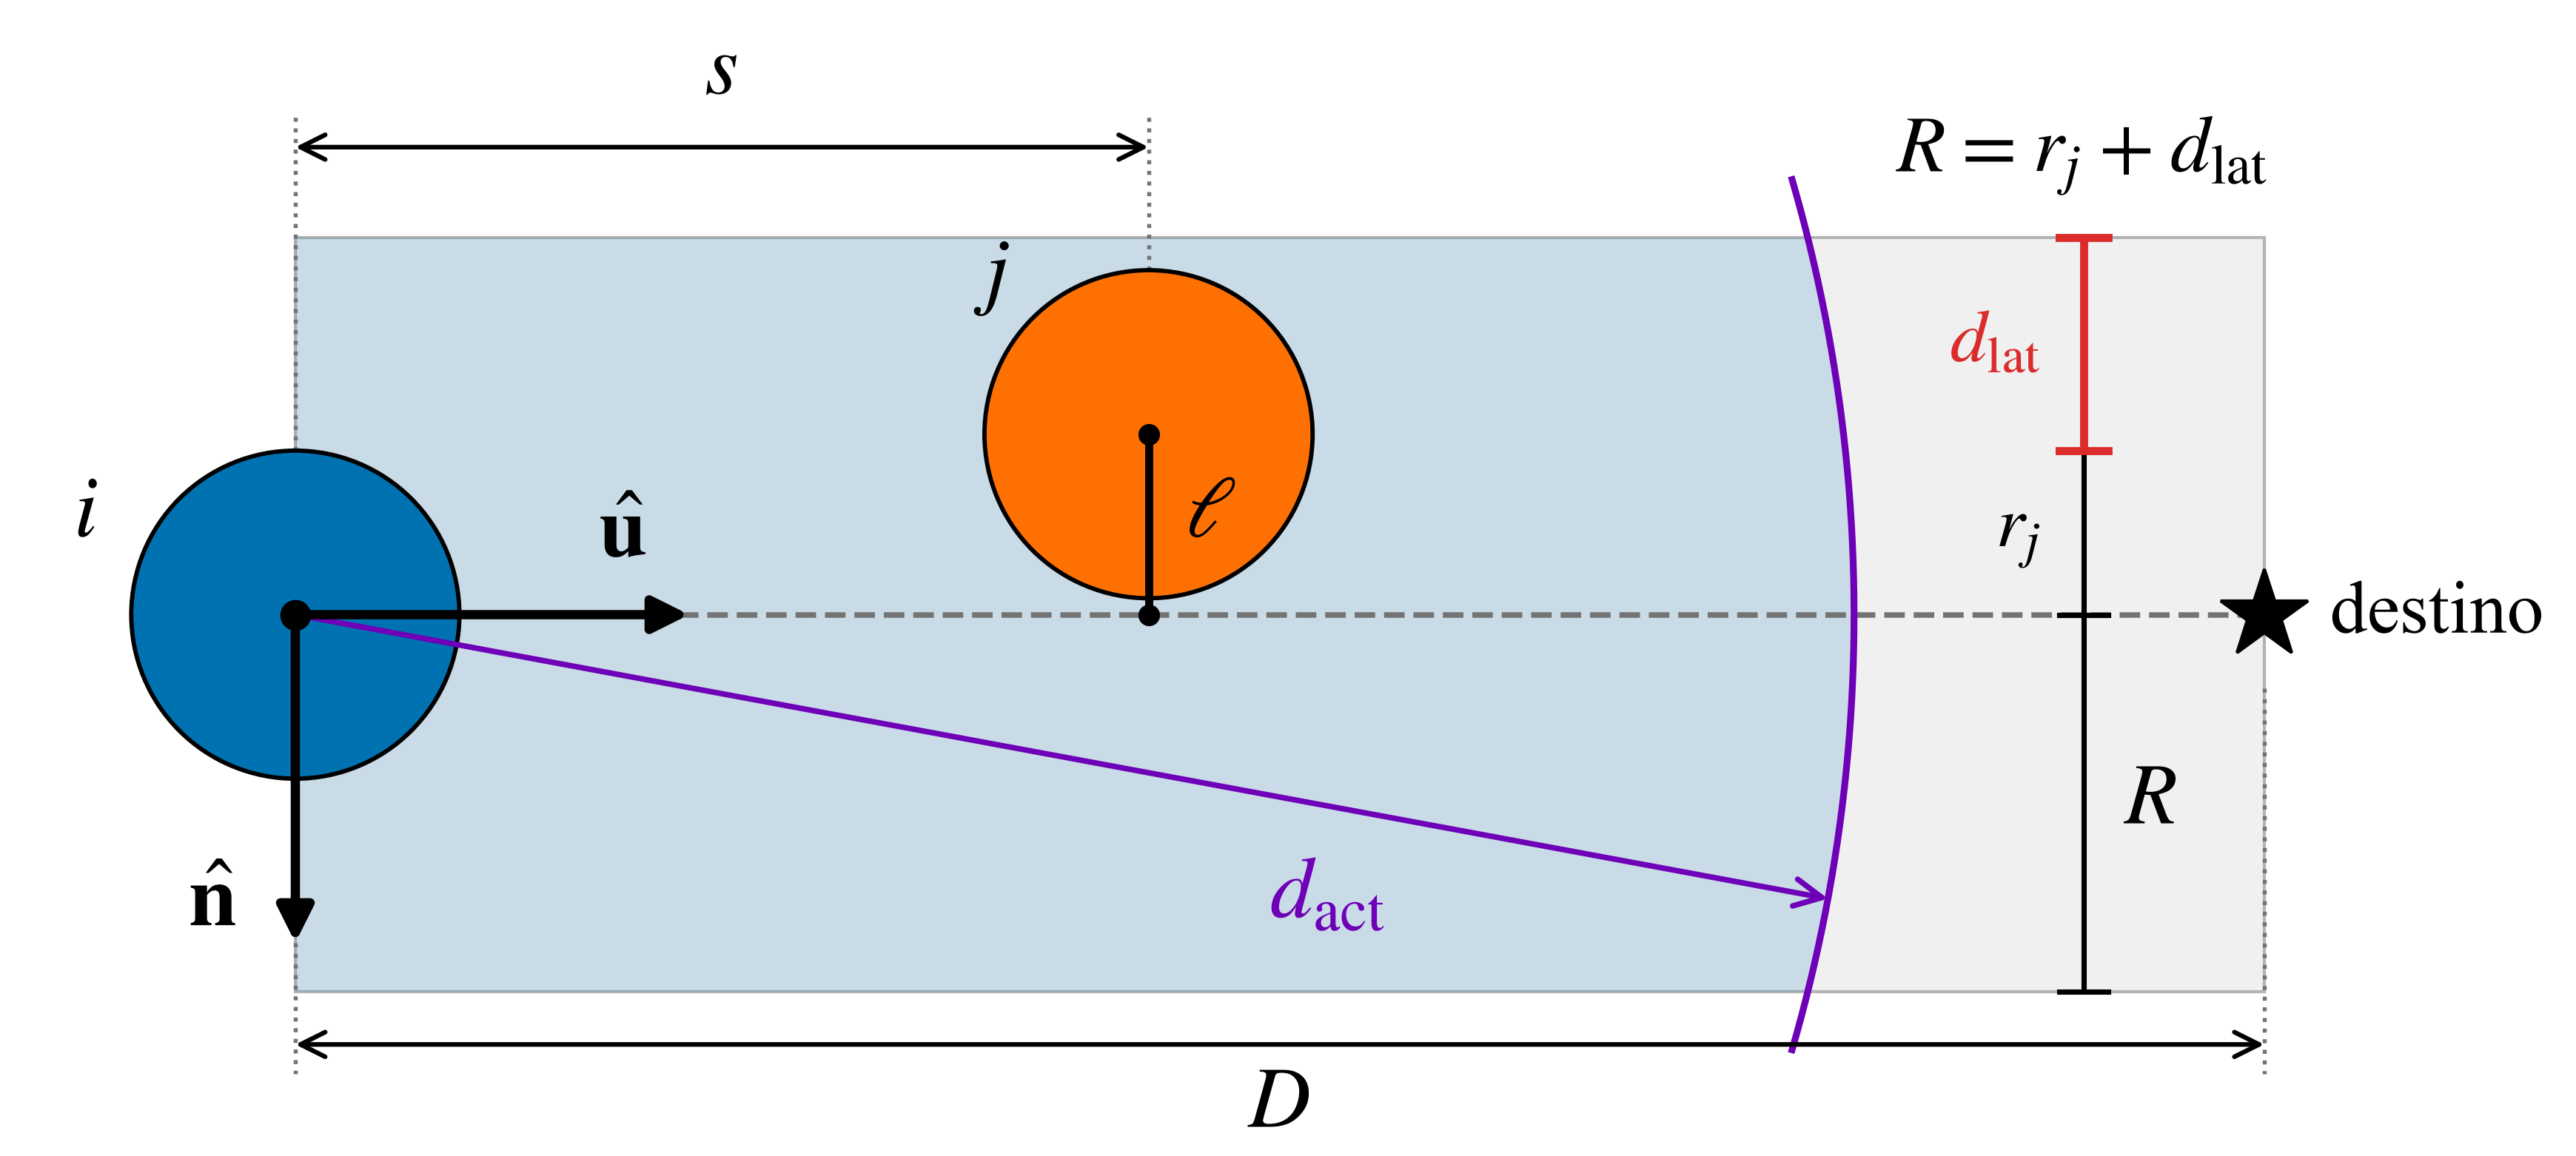
\includegraphics[width=\linewidth,height=0.62\textheight,keepaspectratio]{elusion_deteccion.png}
  \vspace{2pt}

  \large
  Conflicto entre $i$ y $j$:
  \[
    d_{ij} \leq \dact, \qquad 0 < s < D, \qquad |\ell| < R = r_j + \dlat
  \]
\end{frame}

\begin{frame}{Fundamentos}
  \framesubtitle{Capa de elusión: ¿qué hace?}
  \centering
  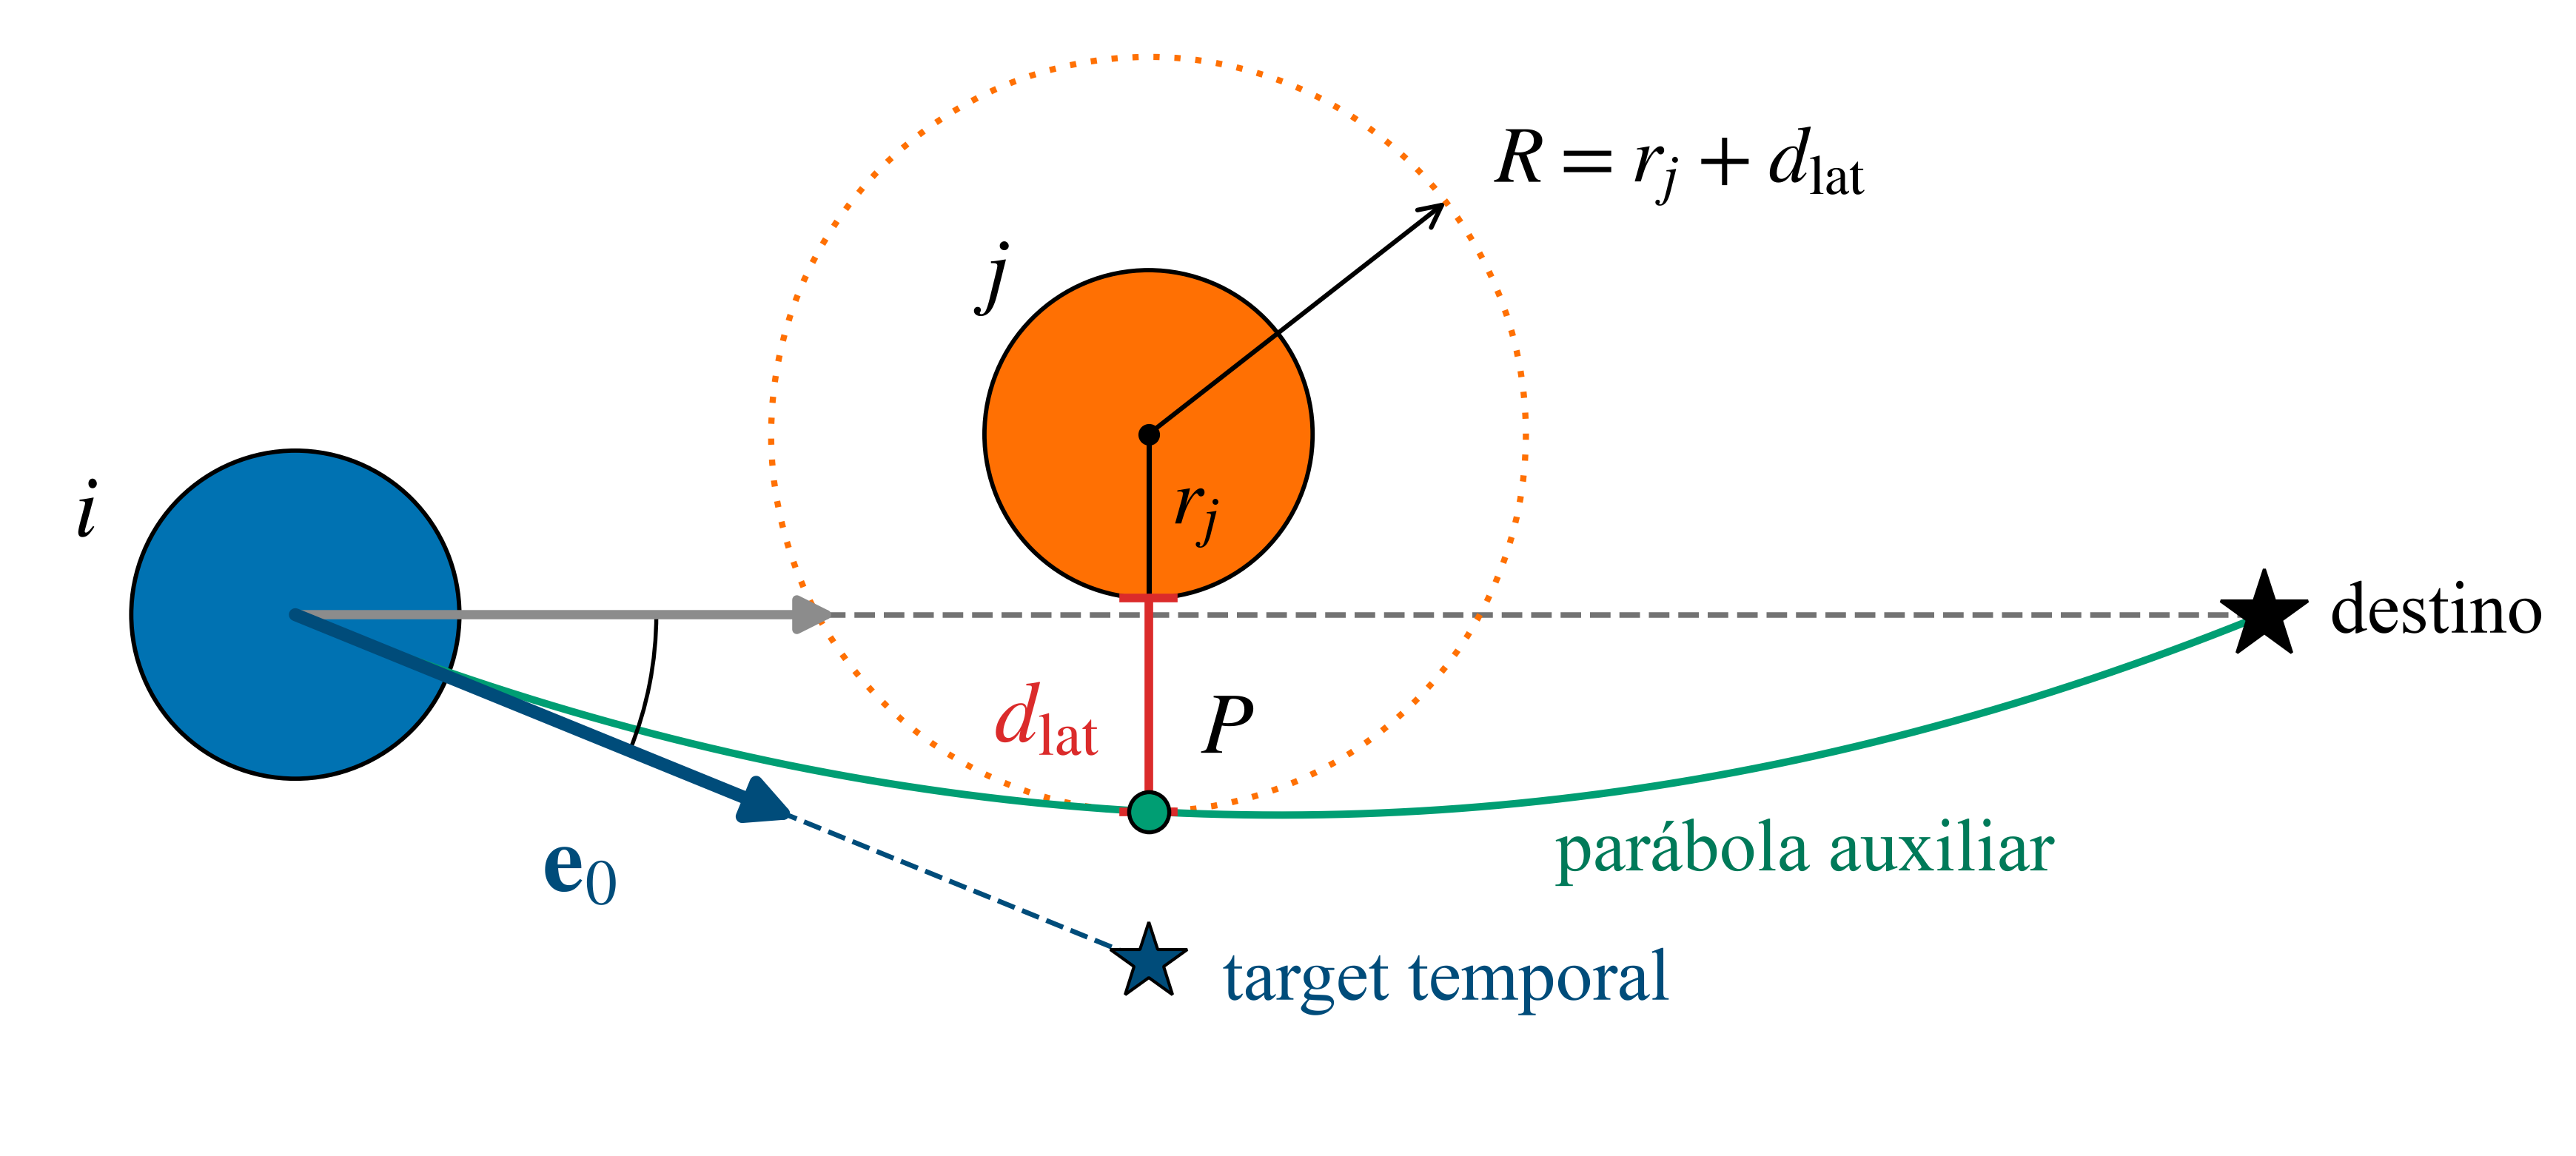
\includegraphics[width=\linewidth,height=0.60\textheight,keepaspectratio]{elusion_activacion.png}
  \vspace{2pt}

  \large
  \[
    y'(0) = \frac{(\ell + R)\,D}{s\,(D - s)}
    \qquad\Rightarrow\qquad
    \vv{e}_0 = \frac{\hat{\vv{u}} + y'(0)\,\hat{\vv{n}}}{\sqrt{1 + y'(0)^2}}
  \]
\end{frame}


\section{Implementación}
\begin{frame}{Implementación}
  \framesubtitle{Motor de simulación}
  \begin{algorithmic}[1]
    \Require $\vv{r}_i(0)$, $\vv{v}_i(0)$, target final y $v_{di}$ de cada peatón, $t_f$, $dt$, $dt_2$
    \State $n \gets \mathrm{round}(dt_2/dt)$, \quad $dt \gets dt_2/n$
    \For{$k = 1,\, 2,\, \dots,\, t_f/dt_2$}
      \For{$n$ pasos de integración}
        \For{cada peatón $i$}
          \State $\vv{e}^{\,target}_i \gets$ hacia target temporal si hay conflicto; si no, hacia target final
          \State $\vv{F}_i \gets \vv{F}_{Di} + \vv{F}_{Gi}$
        \EndFor
        \State $\vv{v}_i \gets \vv{v}_i + (\vv{F}_i/m_i)\,dt$
        \State $\vv{r}_i \gets \vv{r}_i + \vv{v}_i\,dt$
      \EndFor
      \State guardar $t = k\,dt_2$, $\vv{r}_i$, $\vv{v}_i$
    \EndFor
  \end{algorithmic}
\end{frame}

\begin{frame}{Implementación}
  \framesubtitle{Elección del paso de simulación}
  \centering
  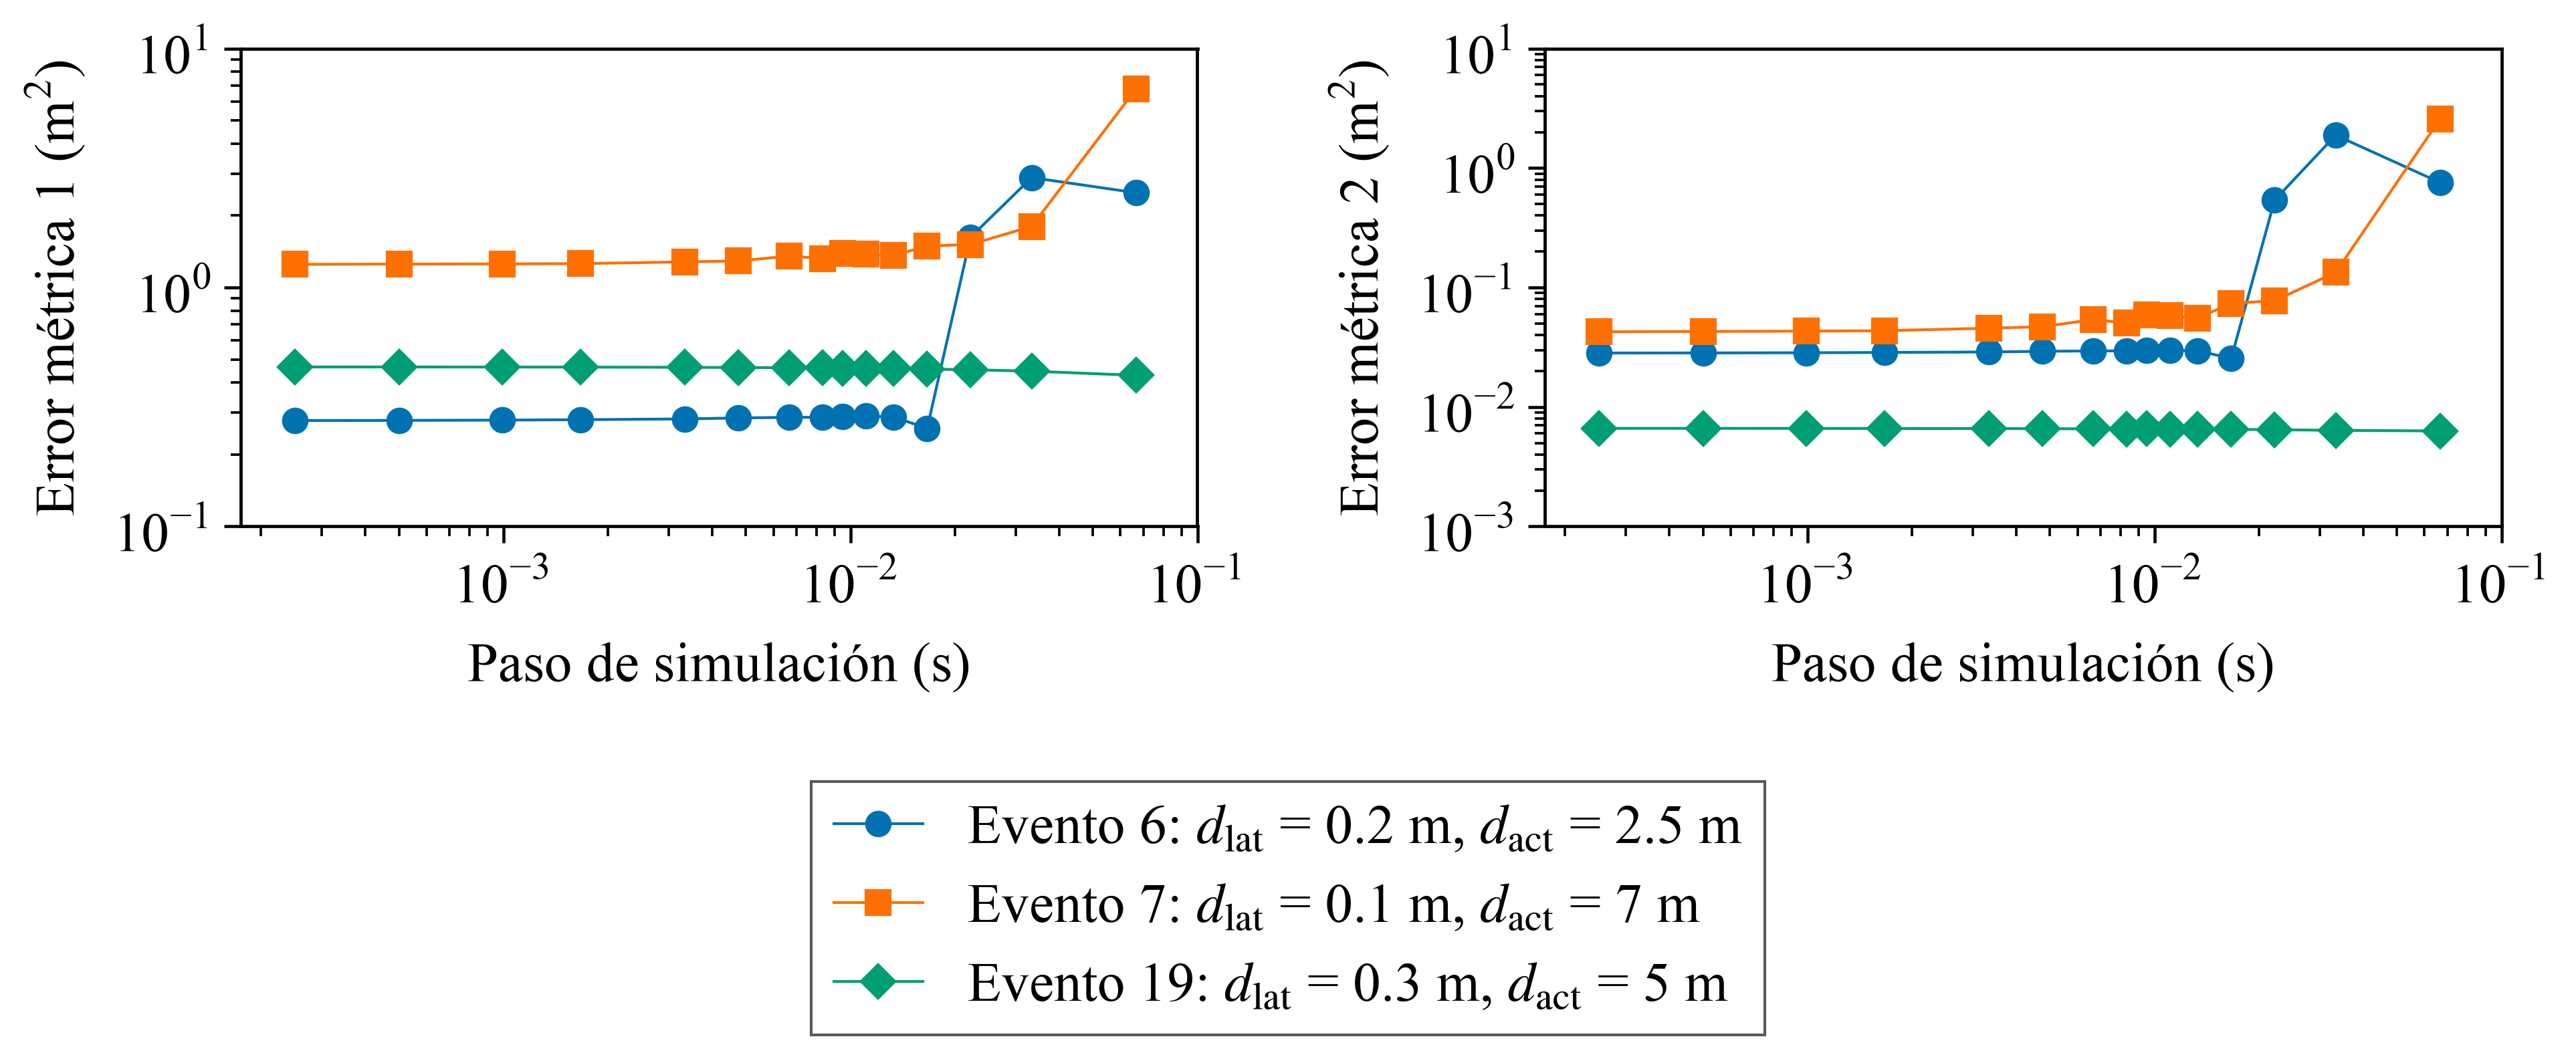
\includegraphics[width=\linewidth,height=0.70\textheight,keepaspectratio]{dt_convergencia.png}

  \vspace{4pt}
  {\large Paso de simulación $dt = 10^{-3}\uni{s}$; \quad paso para guardar estado $dt_2 = \Delta t_{exp}$}
\end{frame}


\section{Simulaciones}
\begin{frame}{Simulaciones}
  \framesubtitle{Sistema: dos peatones en curso de colisión}
  \begin{columns}[c]
    \begin{column}{0.64\textwidth}
      \centering
      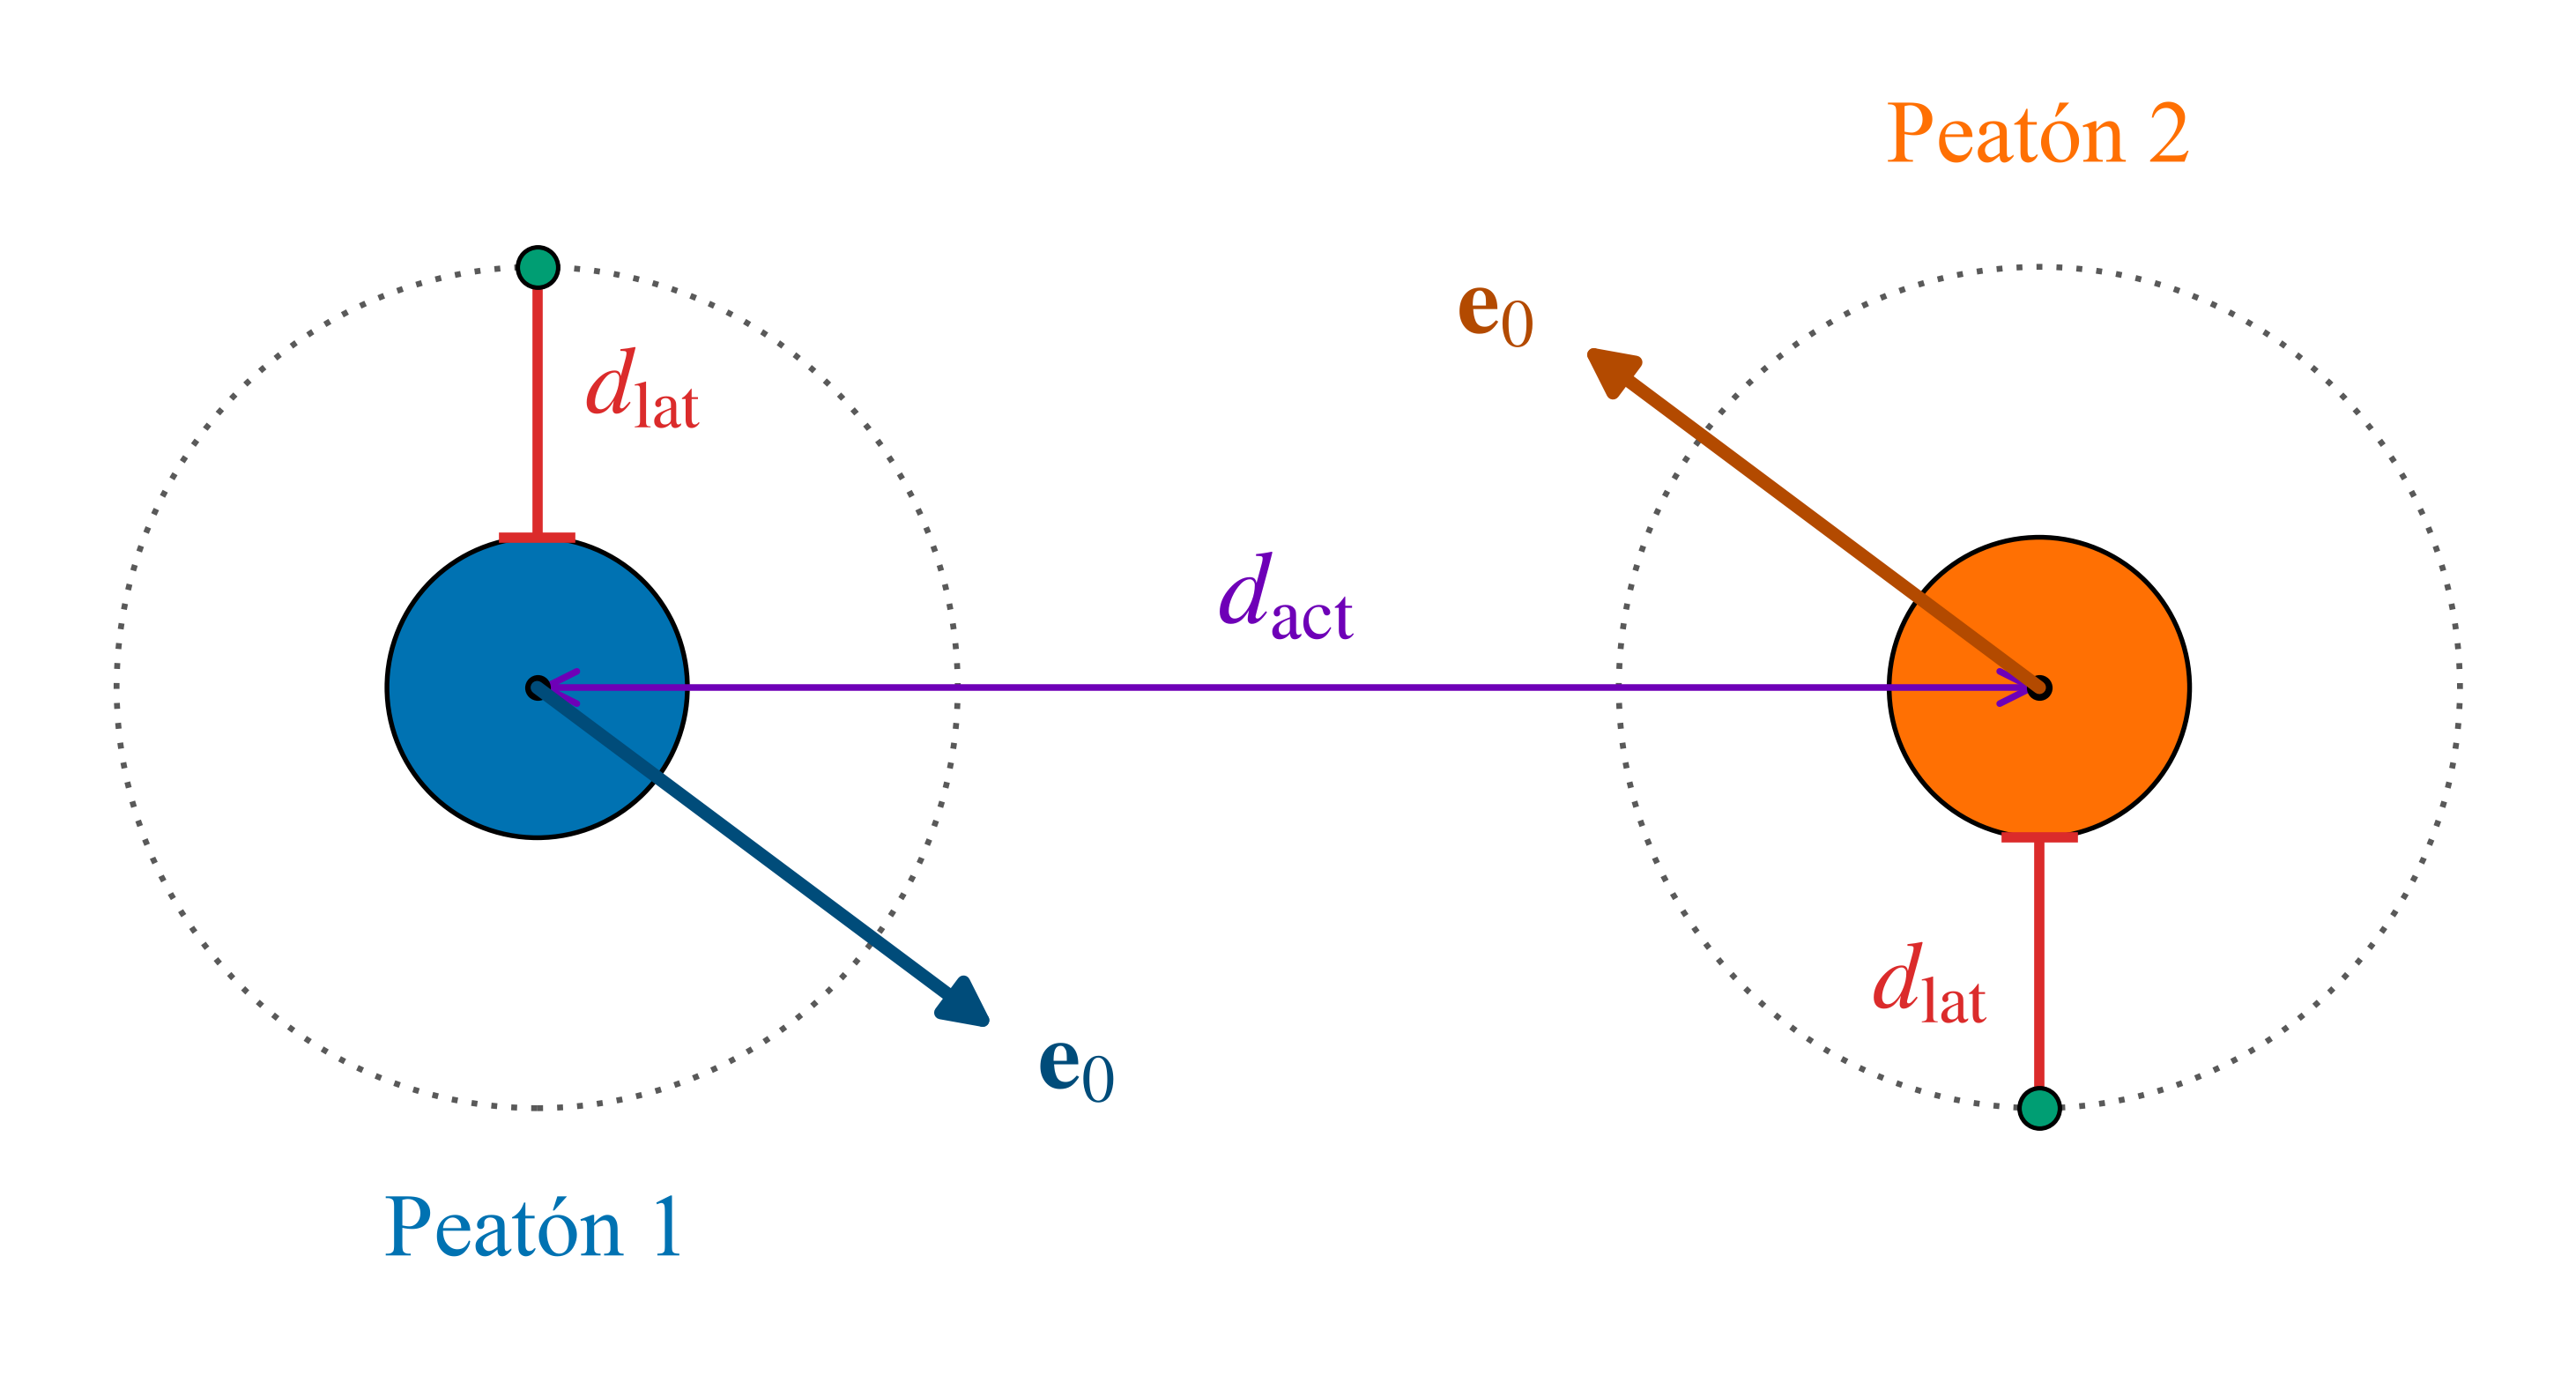
\includegraphics[width=\linewidth,height=0.72\textheight,keepaspectratio]{cuadro_inicial.png}
    \end{column}
    \begin{column}{0.33\textwidth}
      \begin{beamercolorbox}[wd=\linewidth,sep=8pt,rounded=true]{block body alerted}
        \small\textbf{Parámetros a calibrar}\par\vspace{6pt}
        $p_1 = d_{\mathrm{lat}}$: margen lateral de referencia\par\vspace{6pt}
        $p_2 = d_{\mathrm{act}}$: distancia de activación de la elusión
      \end{beamercolorbox}
    \end{column}
  \end{columns}
\end{frame}

\begin{frame}{Simulaciones}
  \framesubtitle{Eventos experimentales y parámetros fijos}
  \begin{columns}[c]
    \begin{column}{0.54\textwidth}
      \begin{beamercolorbox}[wd=\linewidth,sep=8pt,rounded=true]{block body}
        \small\textbf{Eventos experimentales}\par\vspace{4pt}
        \begin{itemize}\setlength{\itemsep}{6pt}
          \item $M = 18$ eventos, intervalo de muestreo $\Delta t_{exp} \approx 0.0666\uni{s}$
          \item Por evento: $\vv{r}_i(0)$, $\vv{v}_i(0)$, $v_{di}$ y $t_f$
          \item Target final: posición inicial del otro peatón
          \item $5$ eventos espejados: $y' = 2\,y_0 - y$
        \end{itemize}
      \end{beamercolorbox}
    \end{column}
    \begin{column}{0.38\textwidth}
      \begin{beamercolorbox}[wd=\linewidth,sep=8pt,rounded=true]{block body}
        \small\textbf{Parámetros fijos}\par\vspace{6pt}
        \renewcommand{\arraystretch}{1.25}
        \begin{tabular}{@{}l@{\qquad}l@{}}
          Radio $r_i$ & $0.25\uni{m}$ \\
          Masa $m_i$ & $80\uni{kg}$ \\
          $\tau_i$ & $0.5\uni{s}$ \\
          $k_n$ & $1.2\ten{5}\uni{N/m}$ \\
          $k_t$ & $2.4\ten{5}\uni{kg/(m\,s)}$ \\
        \end{tabular}\par\vspace{4pt}
        {\footnotesize Helbing et al. (2000)}
      \end{beamercolorbox}
    \end{column}
  \end{columns}
\end{frame}

\begin{frame}{Simulaciones}
  \framesubtitle{Observables}
  Error del peatón $i$ del evento $m$ \ ($N_m$ instantes $t_k = k\,\Delta t_{exp}$):
  \[
    E^{(1)}_i = \frac{1}{N_m}\sum_{k}\big|\vv{r}^{\,exp}_i(t_k) - \vv{r}^{\,sim}_i(t_k)\big|^2
    \qquad\quad
    E^{(2)}_i = \frac{1}{N_m}\sum_{k}\min_{j}\big|\vv{r}^{\,exp}_i(t_k) - \vv{r}^{\,sim}_i(t_j)\big|^2
  \]
  \vspace{2pt}
  Error del evento y error poblacional:
  \[
    E_m = \frac{E_1 + E_2}{2}
    \qquad\quad
    \langle E\rangle(d_{\mathrm{lat}},\,d_{\mathrm{act}}) = \frac{1}{M}\sum_{m=1}^{M} E_m(d_{\mathrm{lat}},\,d_{\mathrm{act}})
  \]
  \vspace{2pt}
  Barra de error: desvío estándar muestral entre eventos, \ $\langle E\rangle \pm \sigma_E$
  \[
    \sigma_E = \sqrt{\frac{1}{M-1}\sum_{m=1}^{M}\big(E_m - \langle E\rangle\big)^2}
  \]
\end{frame}

\begin{frame}{Simulaciones}
  \framesubtitle{Simulaciones realizadas}
  \textbf{Grilla de parámetros}
  \begin{itemize}\setlength{\itemsep}{3pt}
    \item $d_{\mathrm{lat}}$: $0.10$ a $0.50\uni{m}$, paso $0.05\uni{m}$ \ ($9$ valores)
    \item $d_{\mathrm{act}}$: $2.5$ a $7\uni{m}$, paso $0.5\uni{m}$ \ ($10$ valores)
    \item $90$ puntos de grilla $\times$ $18$ eventos $= 1620$ simulaciones
    \item Duración: $t_f$ de cada evento \ ($5.3$ a $8.9\uni{s}$)
  \end{itemize}
  \vspace{8pt}
  \textbf{Estudios} (por métrica)
  \vspace{3pt}

  \centering
  \begin{tabular}{ll}
    \hline
    Calibración poblacional & mínimo de $\langle E\rangle$ en la grilla, $18$ eventos \\
    Calibración individual  & mínimo de $E_m$ en la grilla, por evento \\
    Validación cruzada      & $20$ particiones al azar: $13$ de entrenamiento, $5$ de validación \\
    \hline
  \end{tabular}
\end{frame}


\section{Resultados}
\begin{frame}{Resultados}
  \framesubtitle{Animaciones: experimento y simulación}
  \begin{columns}[T]
    \begin{column}{0.49\textwidth}
      \centering{\small Evento 15 (menor $E^{(2)}_m$)}\par\smallskip
      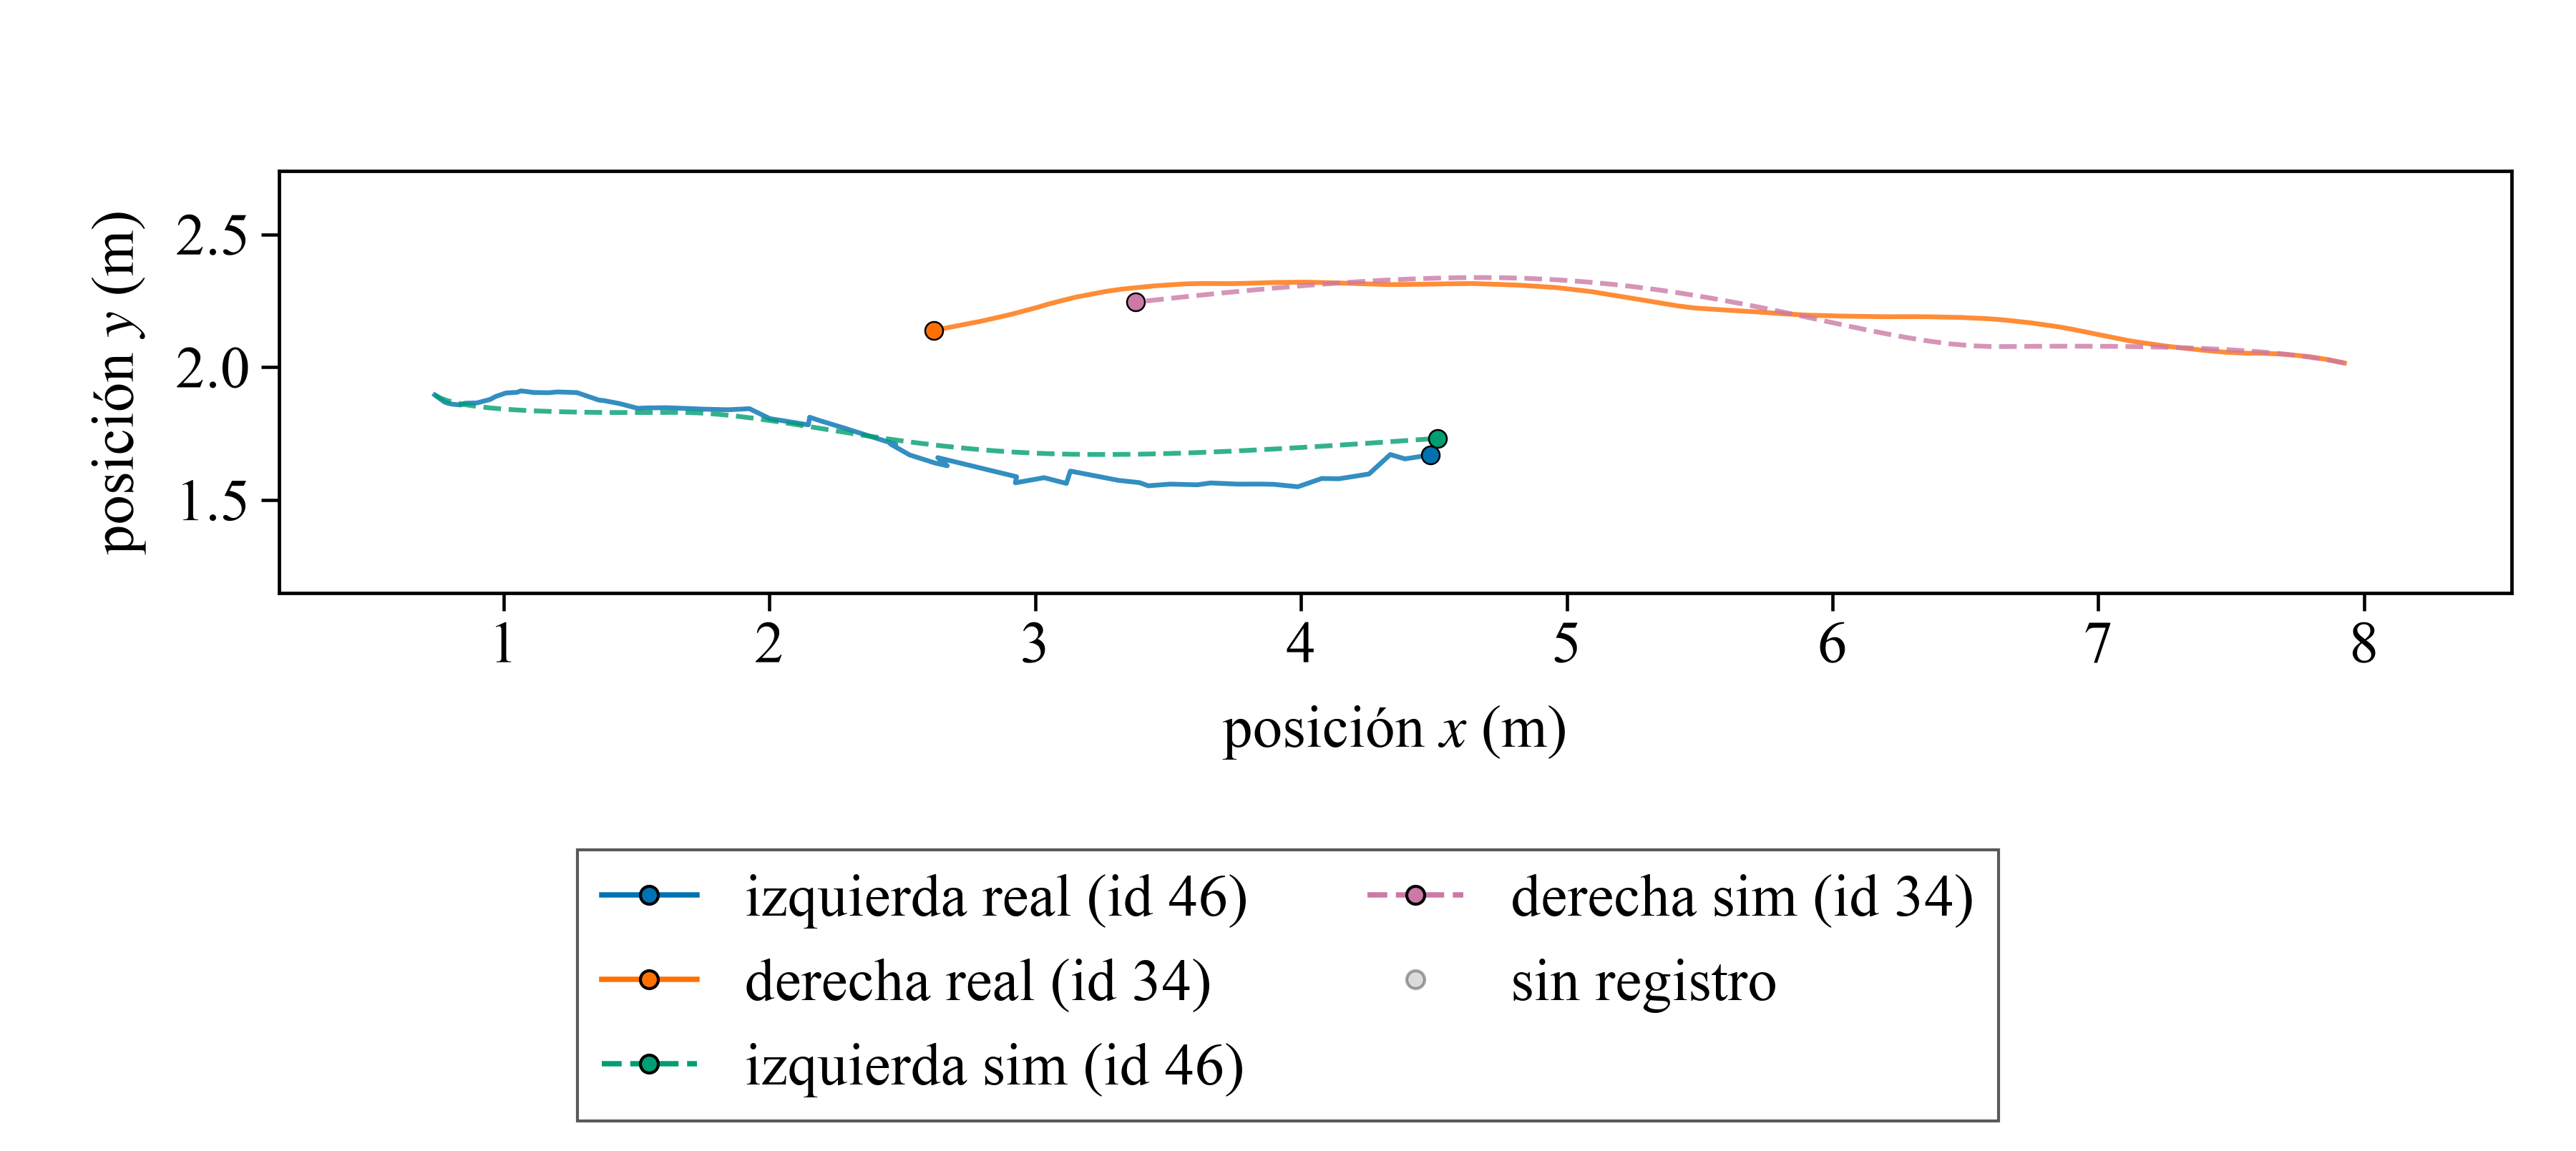
\includegraphics[width=\linewidth,height=0.52\textheight,keepaspectratio]{anim_a.png}
      \par\smallskip{\scriptsize\url{https://youtu.be/PENDIENTE}}
    \end{column}
    \begin{column}{0.49\textwidth}
      \centering{\small Evento 11 (mayor $E^{(2)}_m$)}\par\smallskip
      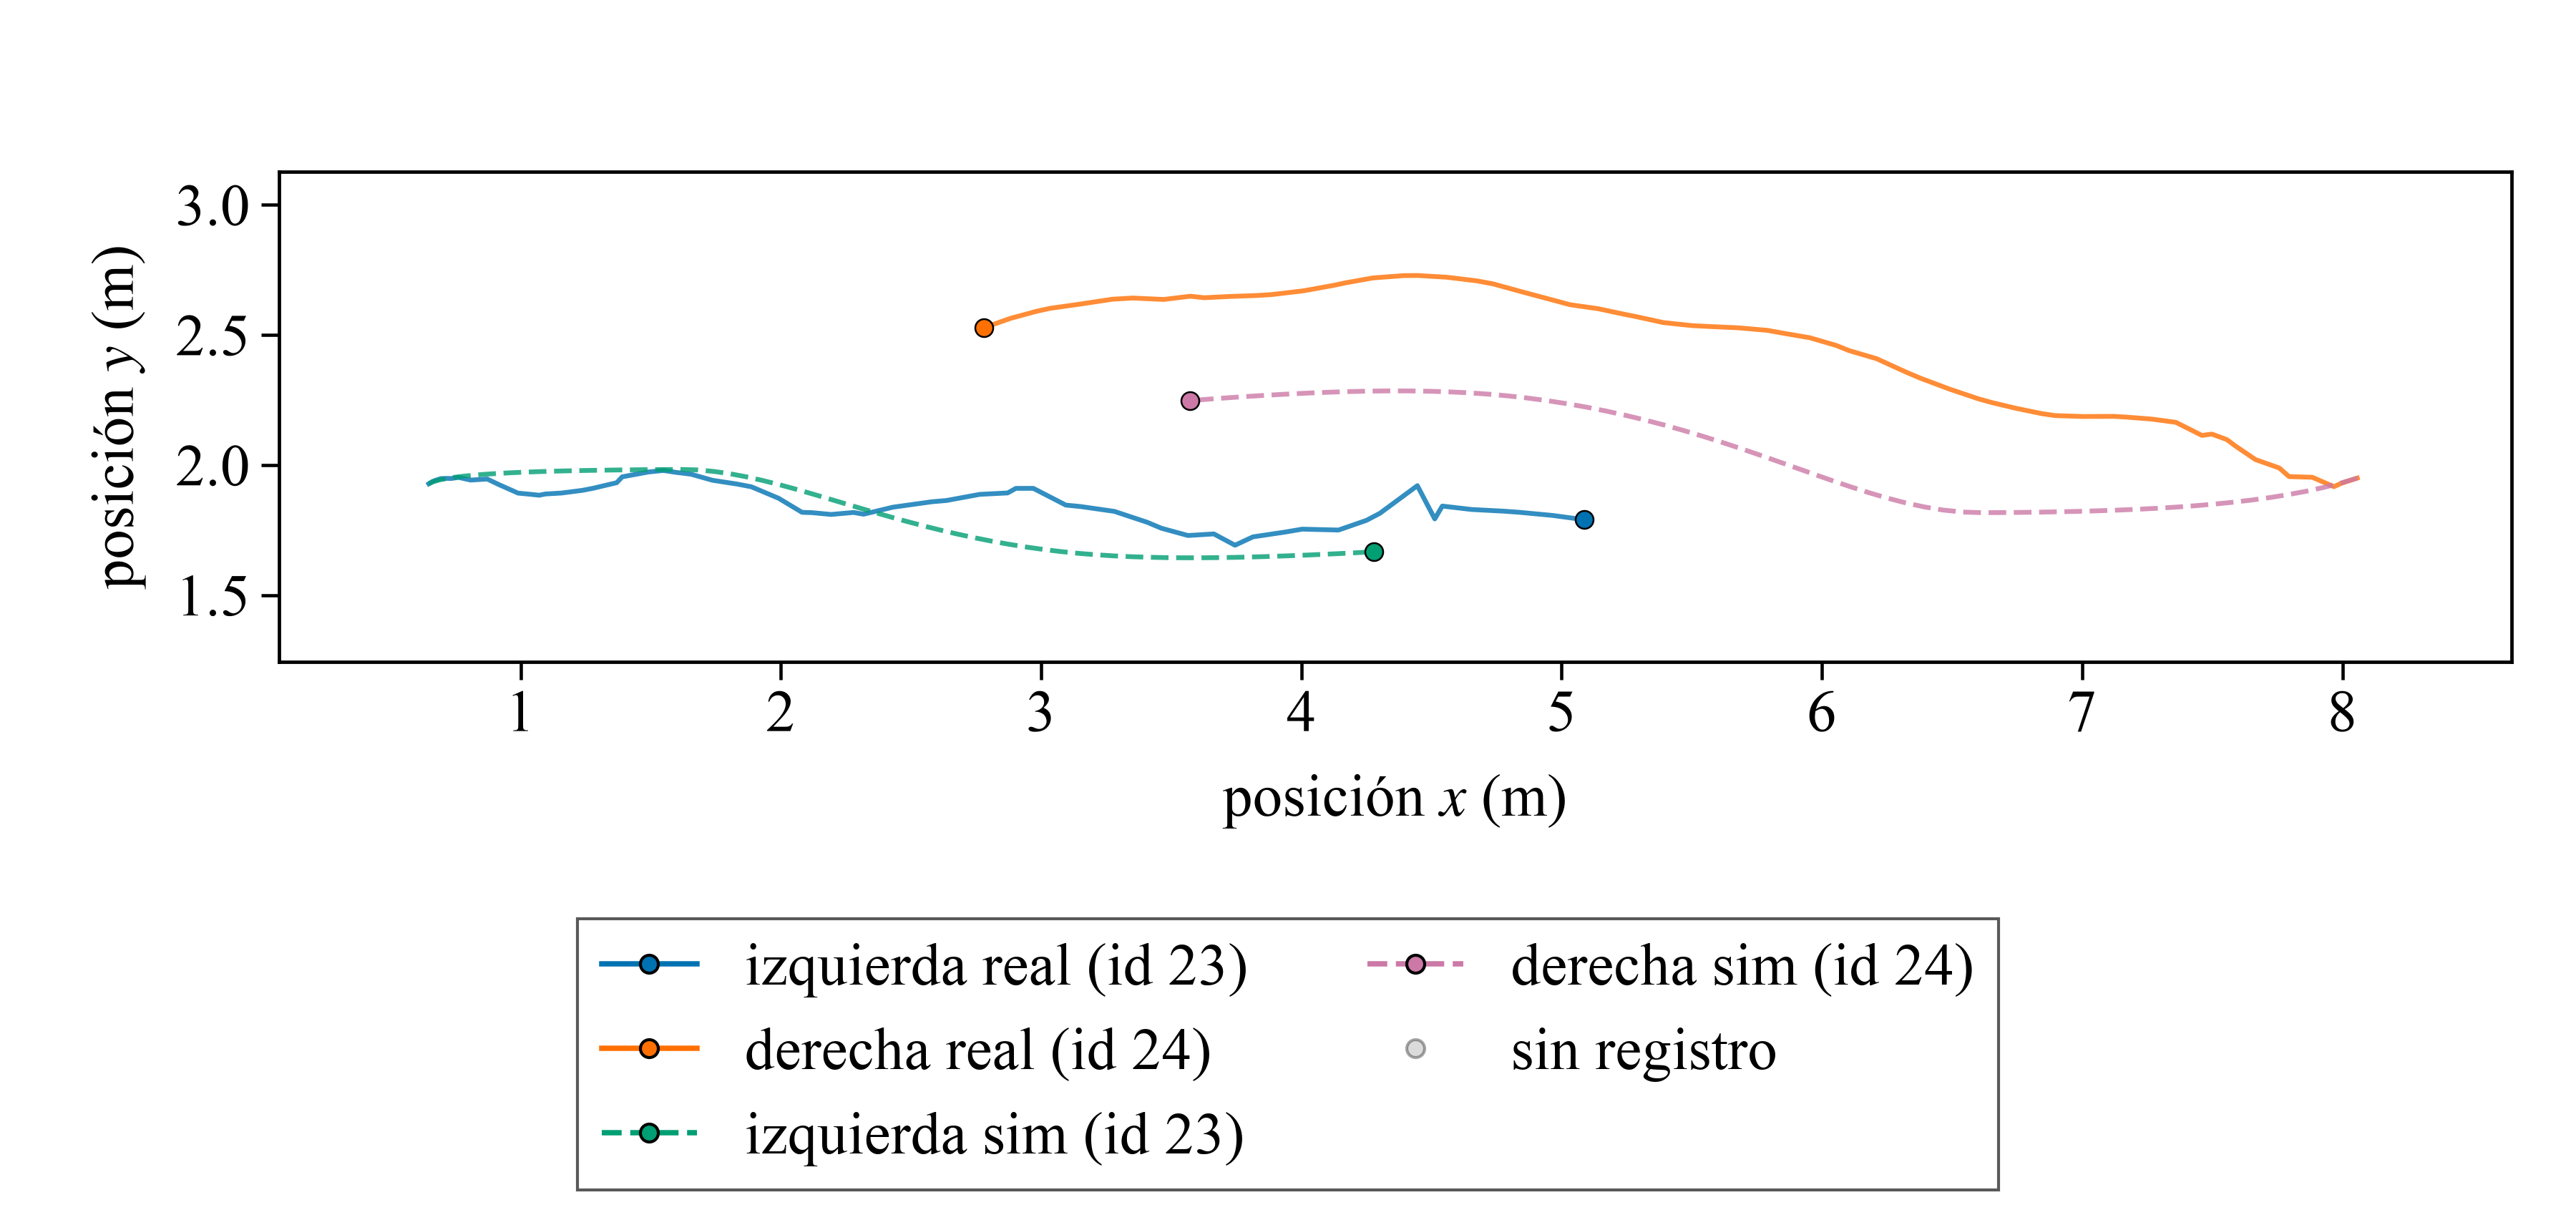
\includegraphics[width=\linewidth,height=0.52\textheight,keepaspectratio]{anim_b.png}
      \par\smallskip{\scriptsize\url{https://youtu.be/PENDIENTE}}
    \end{column}
  \end{columns}
  \vspace{6pt}
  \centering{\small $\dlat = 0.25\uni{m}$, \quad $\dact = 5\uni{m}$}
\end{frame}

\begin{frame}{Resultados}
  \framesubtitle{Trayectorias: experimento y simulación}
  \centering
  {\small Evento 15}\par
  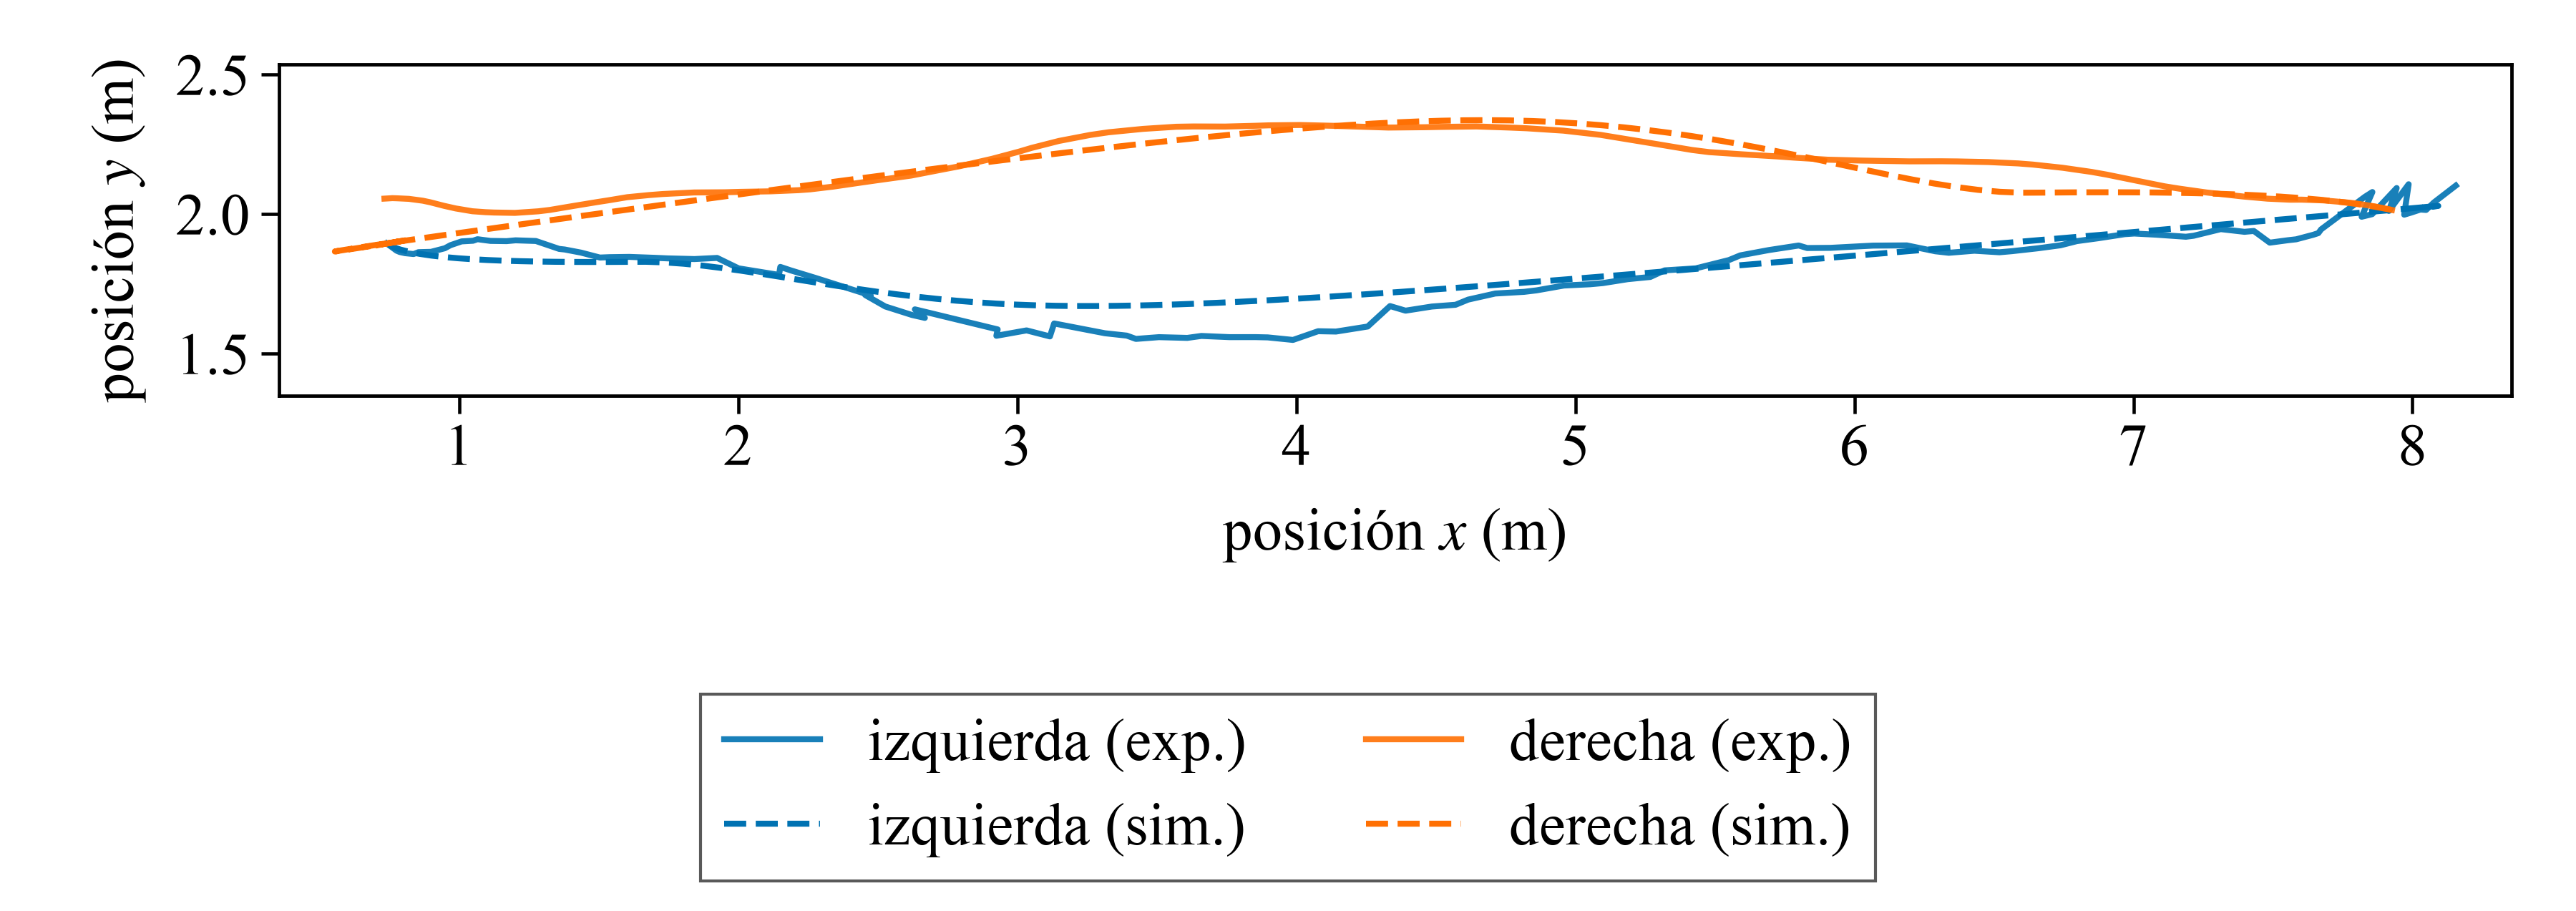
\includegraphics[width=\linewidth,height=0.36\textheight,keepaspectratio]{tray_a.png}\par
  \vspace{2pt}
  {\small Evento 11}\par
  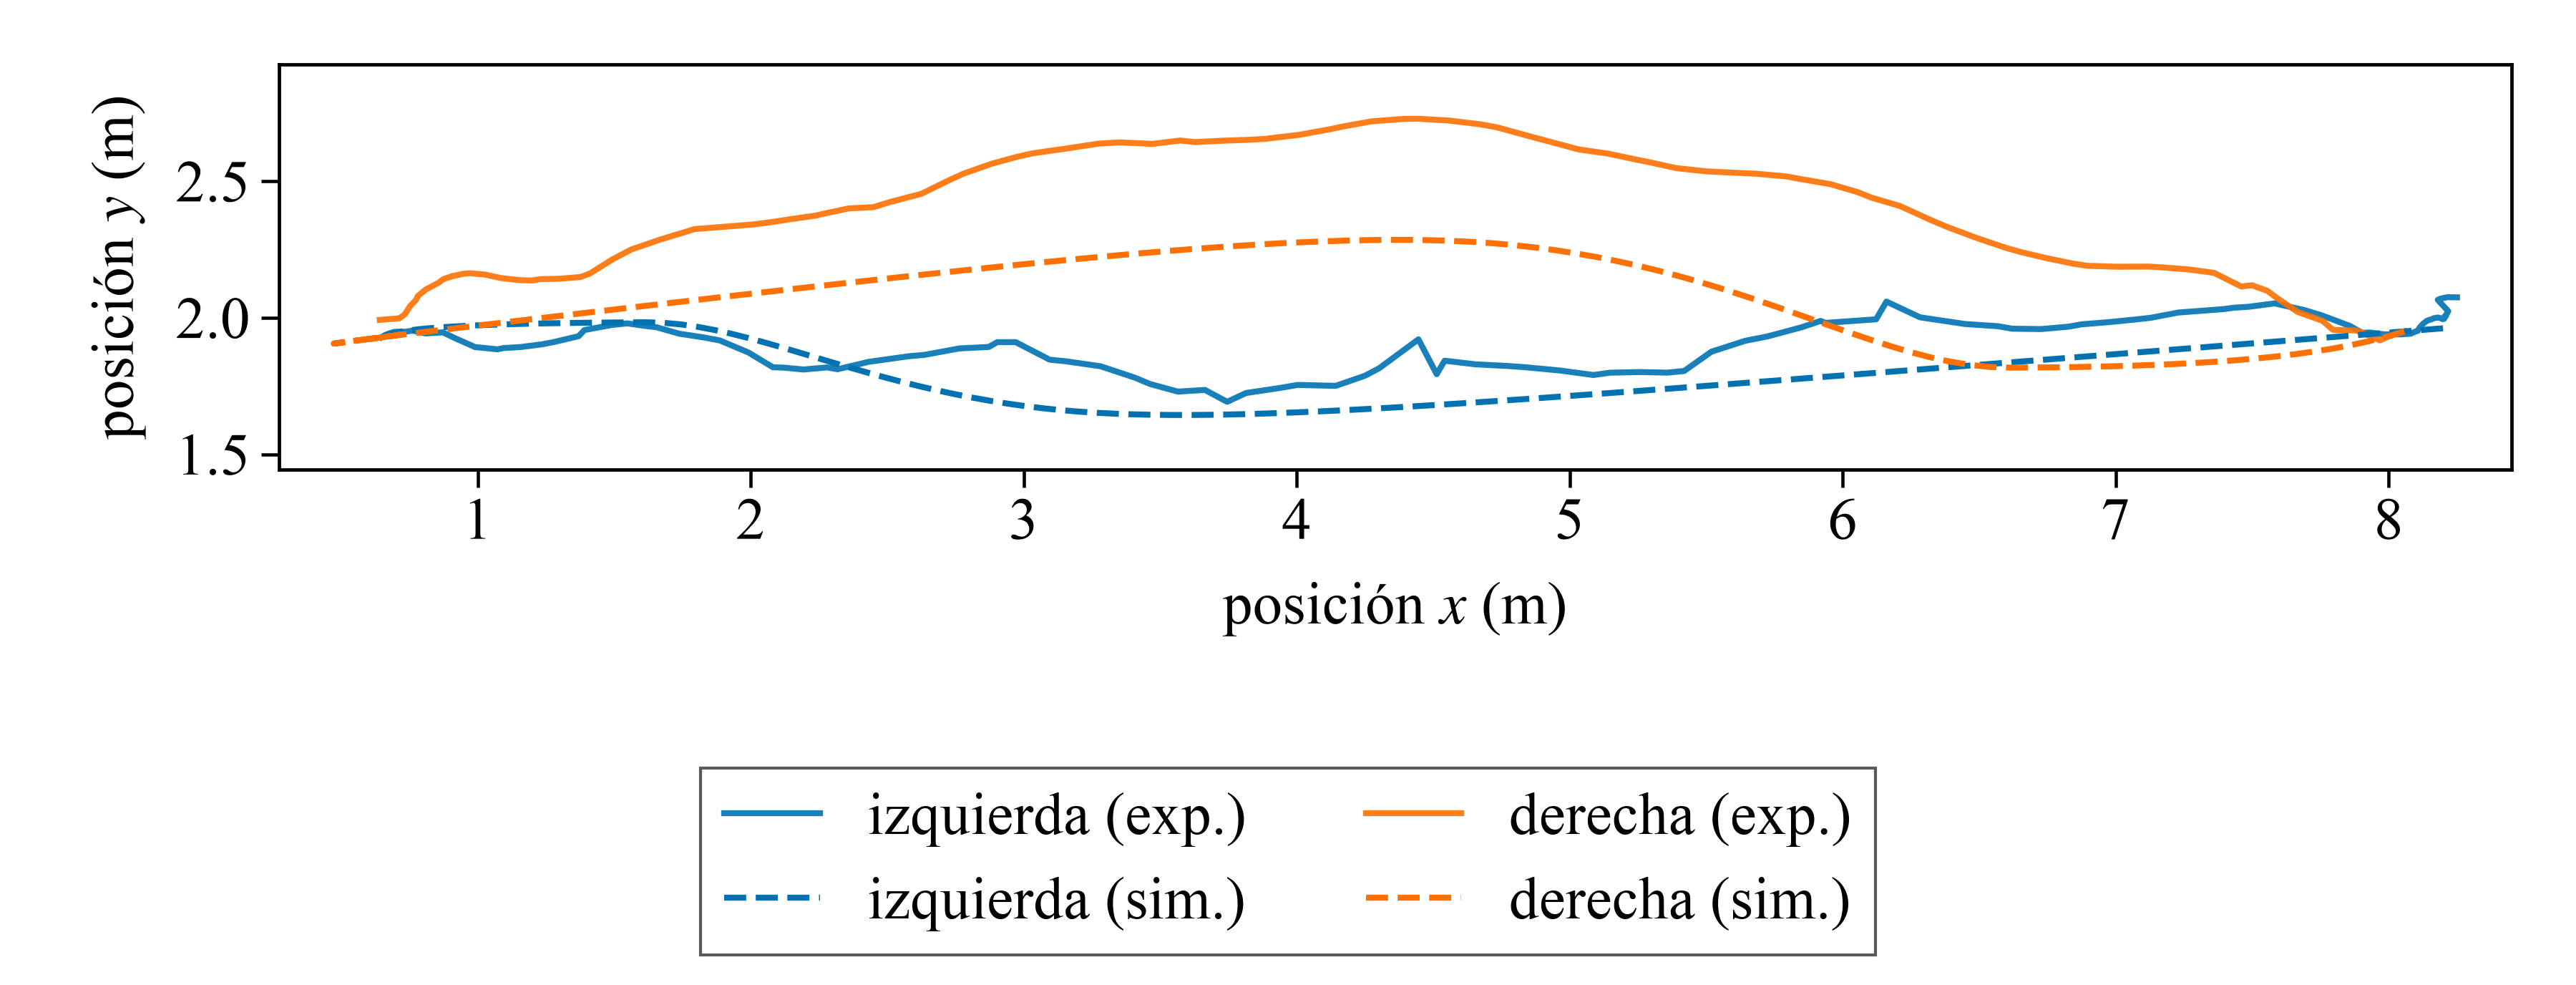
\includegraphics[width=\linewidth,height=0.36\textheight,keepaspectratio]{tray_b.png}
\end{frame}

\begin{frame}{Resultados}
  \framesubtitle{Evolución temporal del observable: métrica 1}
  \begin{columns}[T]
    \begin{column}{0.49\textwidth}
      \centering{\small Evento 15}\par\smallskip
      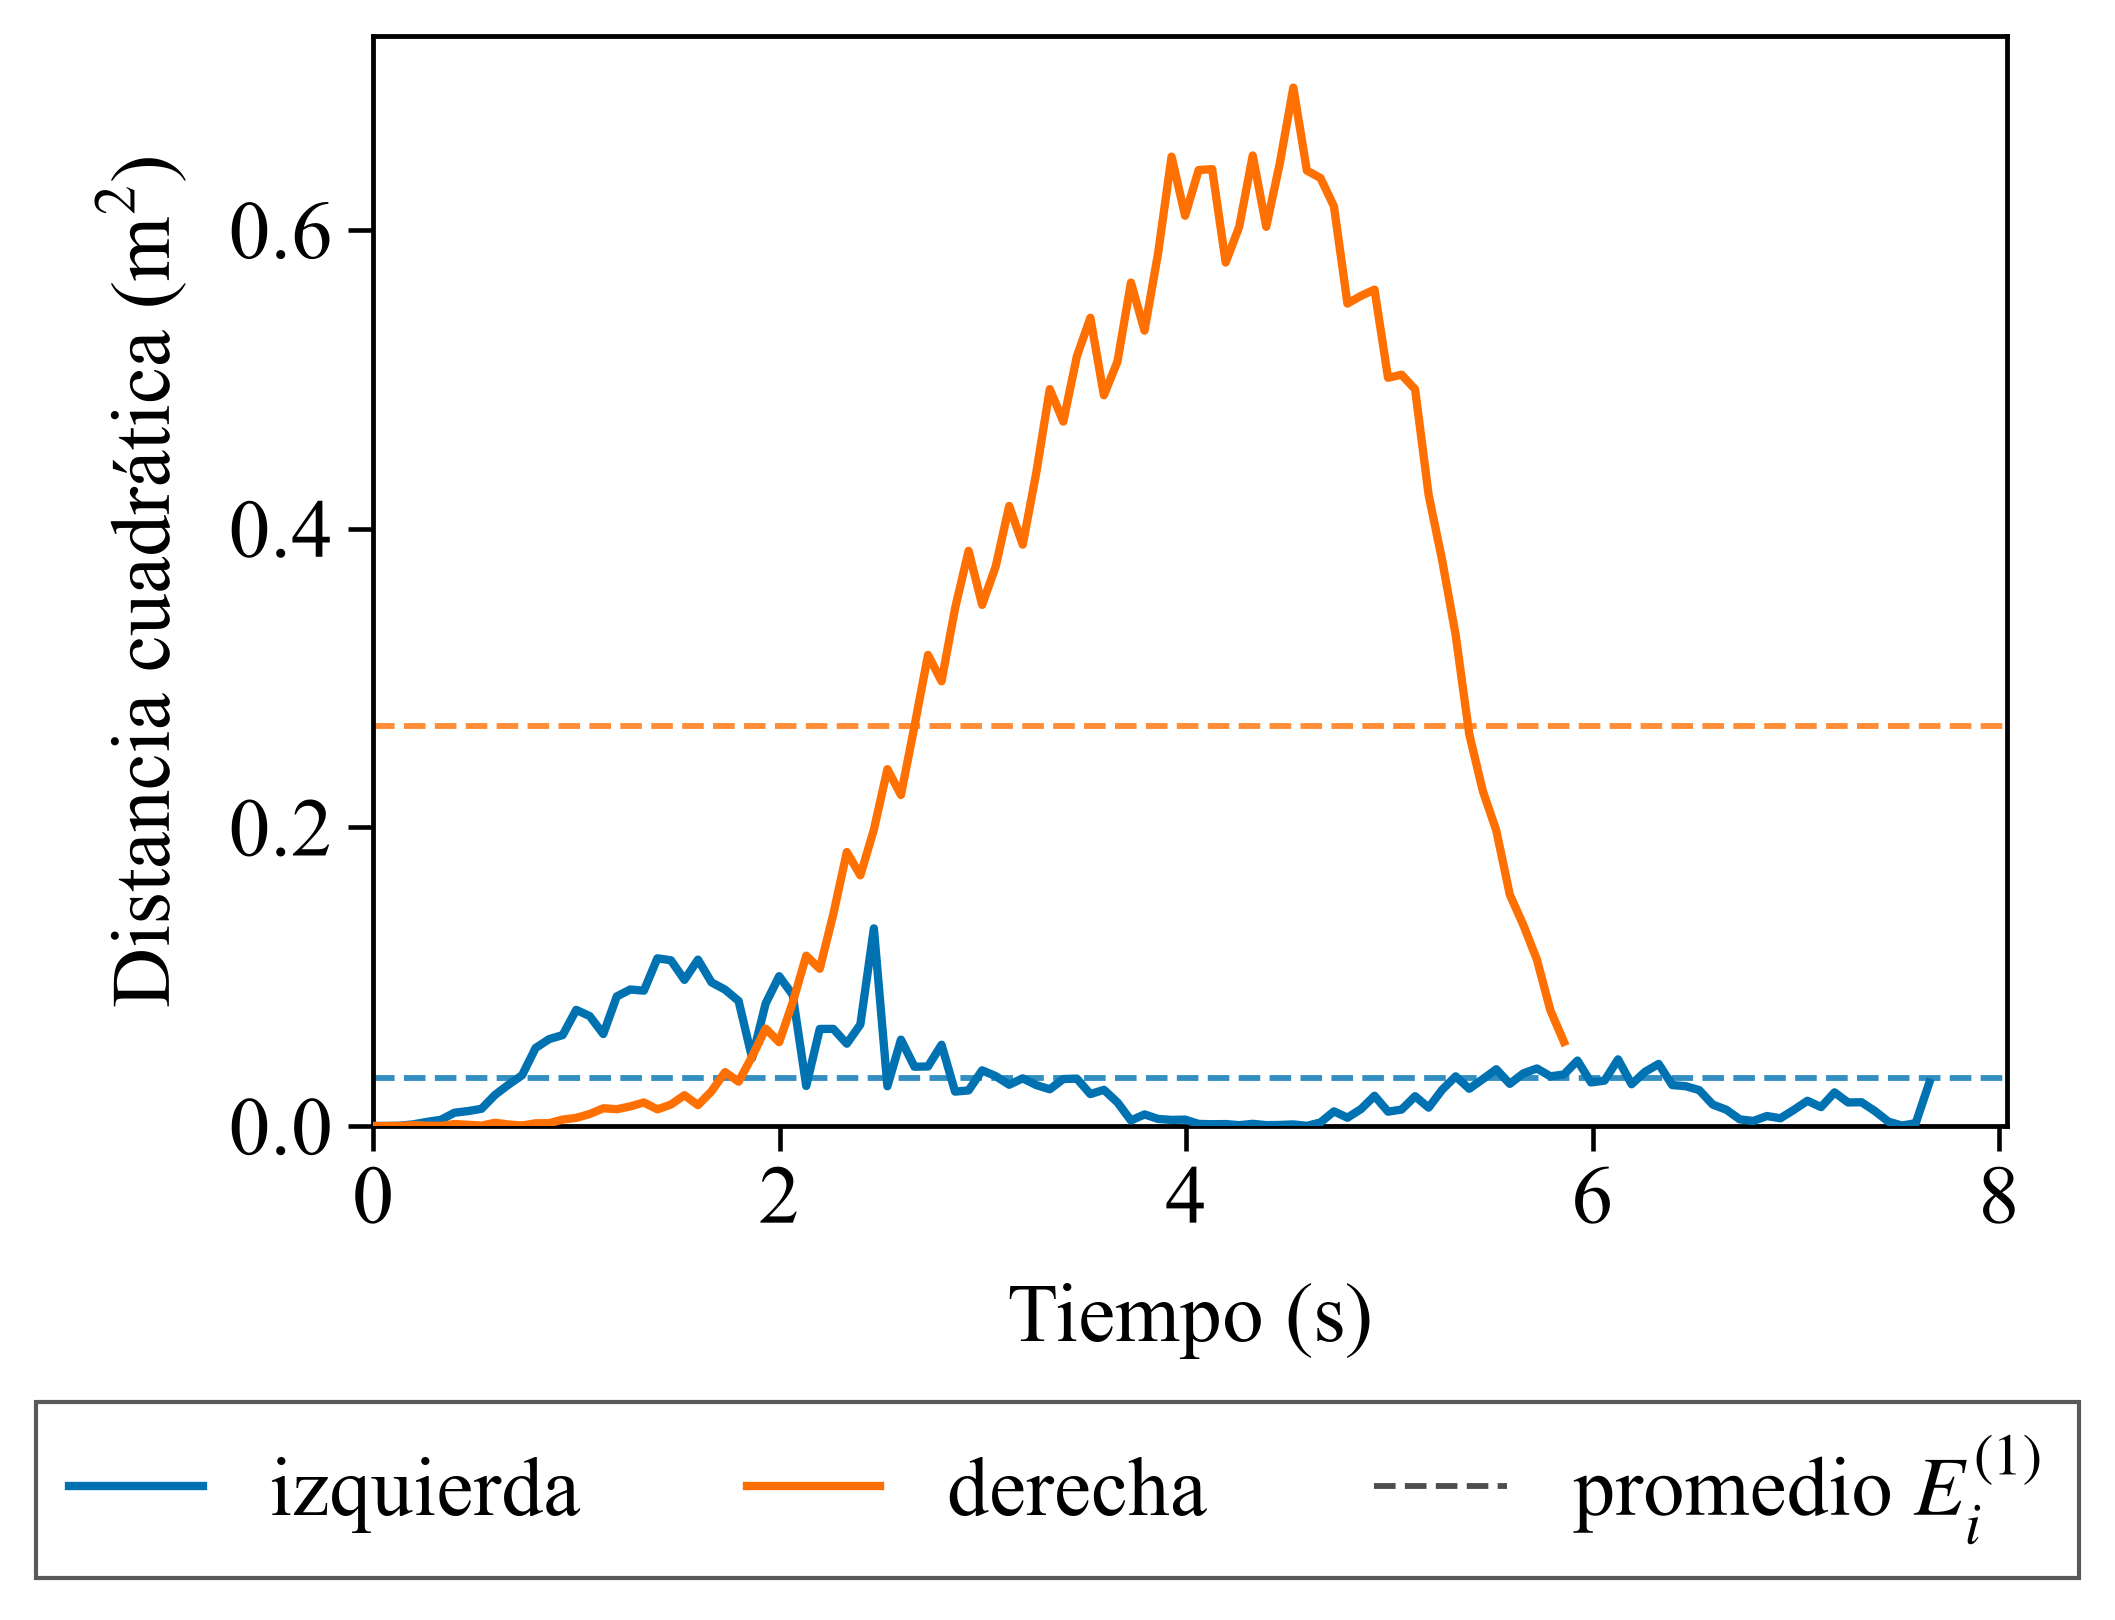
\includegraphics[width=\linewidth,height=0.60\textheight,keepaspectratio]{evol_E1_a.png}
    \end{column}
    \begin{column}{0.49\textwidth}
      \centering{\small Evento 11}\par\smallskip
      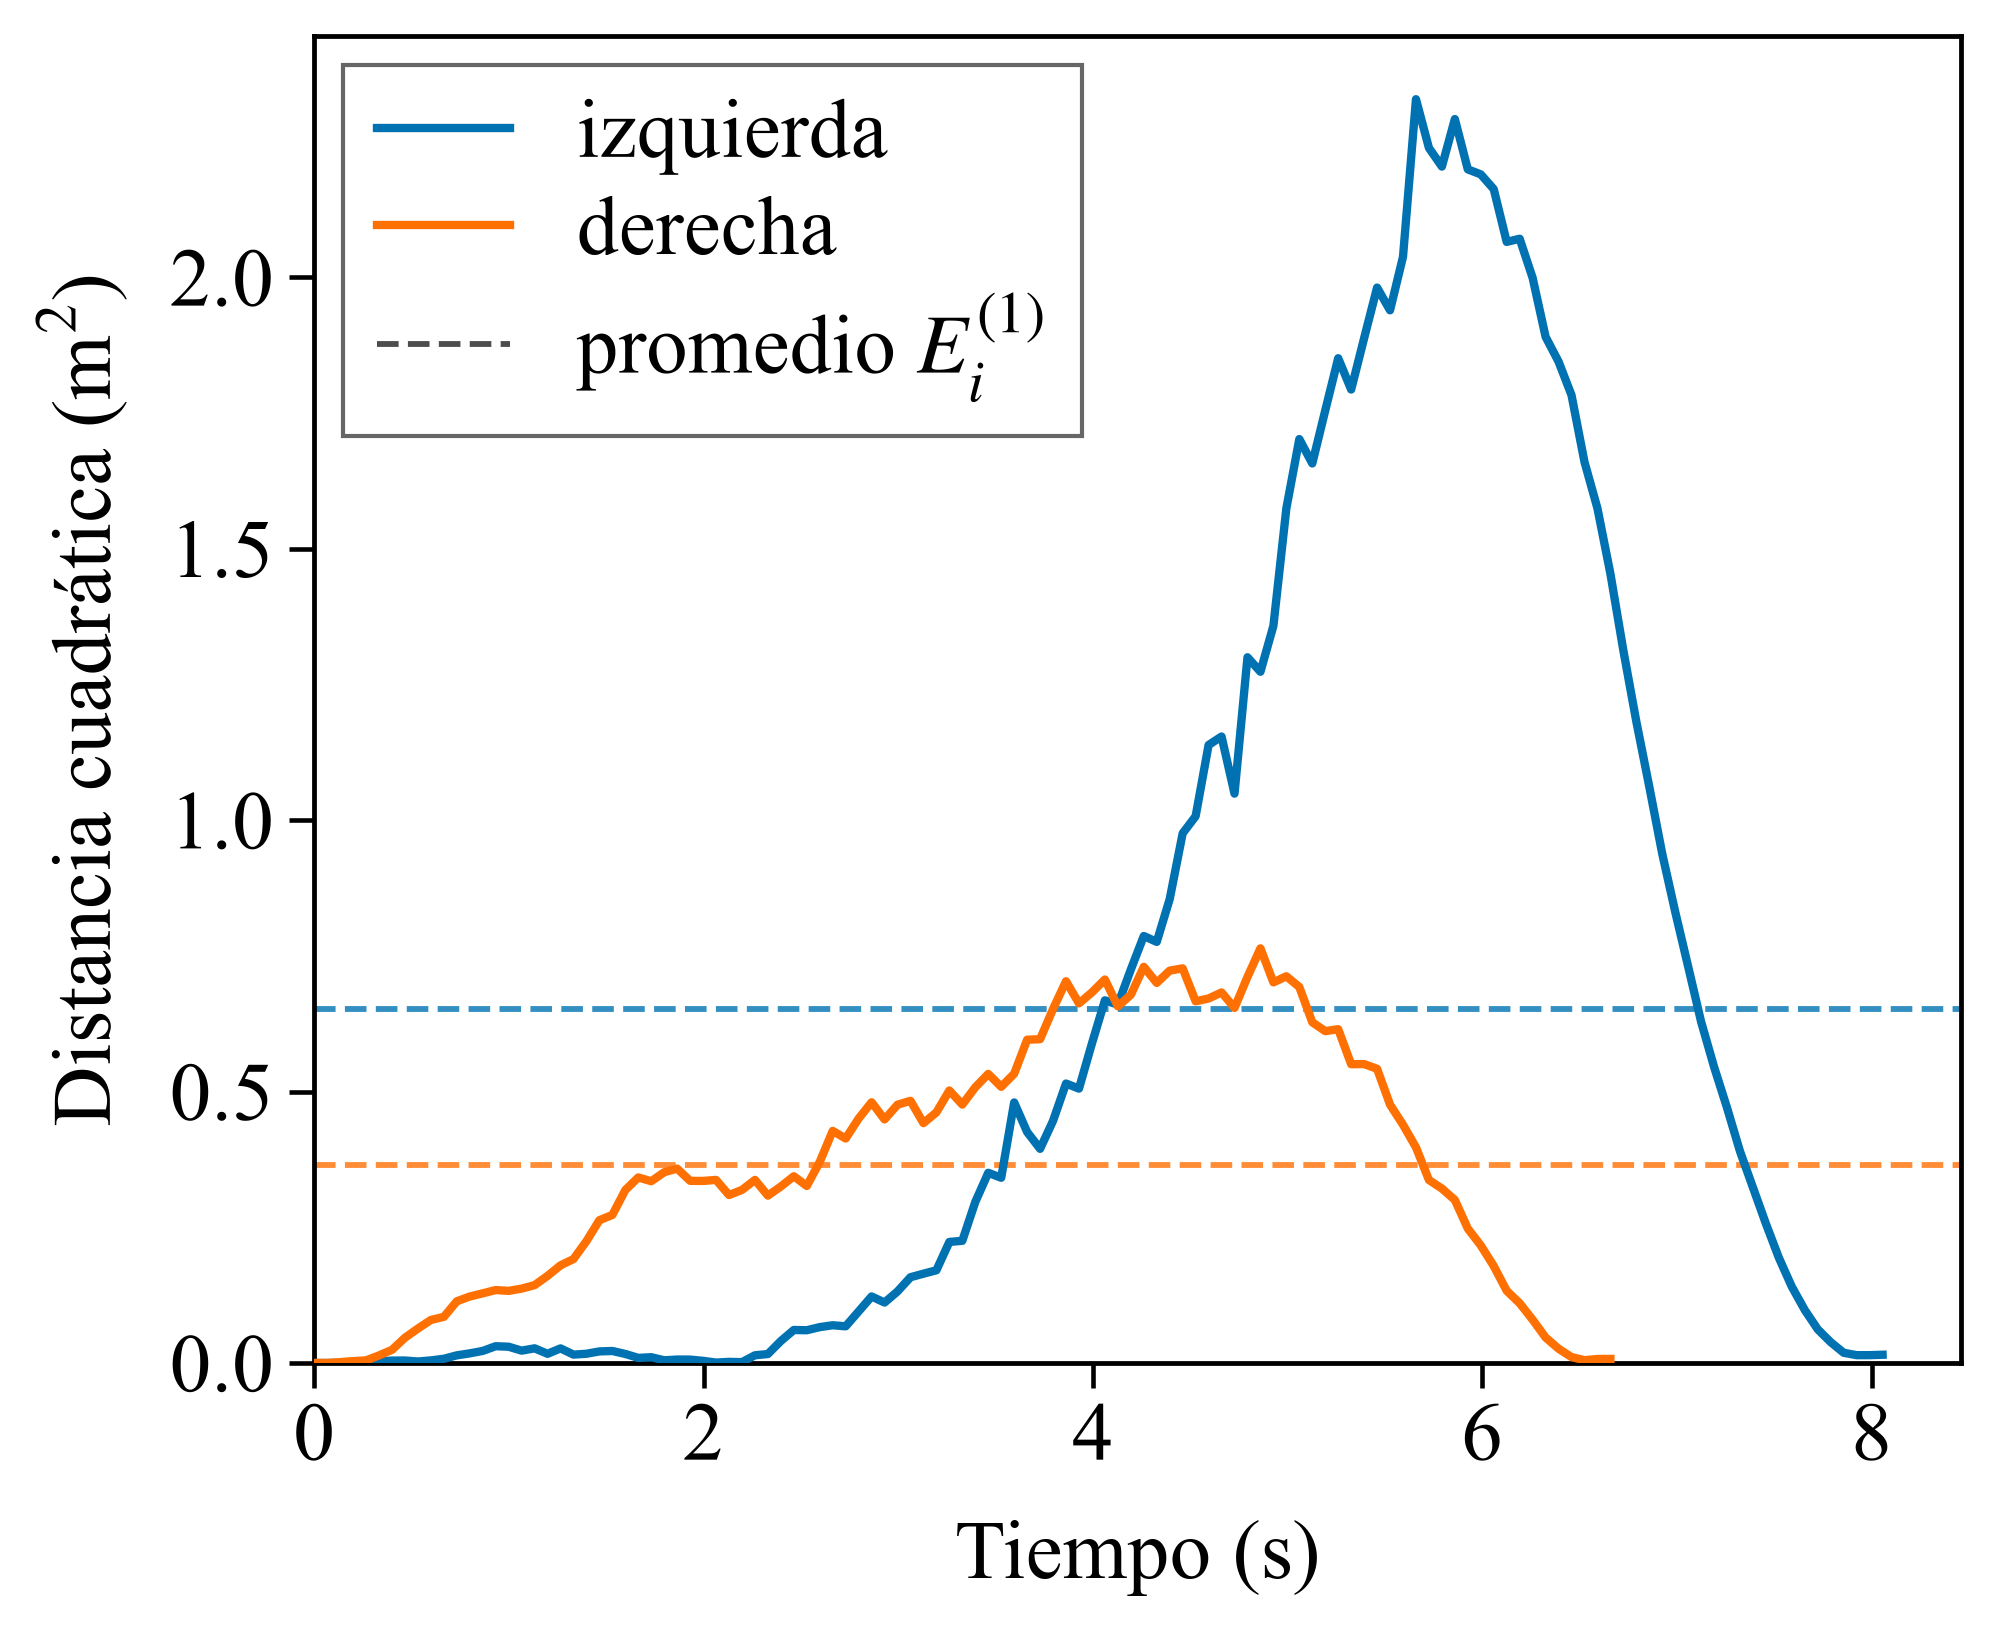
\includegraphics[width=\linewidth,height=0.60\textheight,keepaspectratio]{evol_E1_b.png}
    \end{column}
  \end{columns}
  \vspace{4pt}
  \centering{\small $d^2_i(t_k) = \big|\vv{r}^{\,exp}_i(t_k) - \vv{r}^{\,sim}_i(t_k)\big|^2$, \quad
    punteada: $E^{(1)}_i = \frac{1}{N_m}\sum_k d^2_i(t_k)$, \quad
    $\dlat = 0.25\uni{m}$, \ $\dact = 5\uni{m}$}
\end{frame}

\begin{frame}{Resultados}
  \framesubtitle{Evolución temporal del observable: métrica 2}
  \begin{columns}[T]
    \begin{column}{0.49\textwidth}
      \centering{\small Evento 15}\par\smallskip
      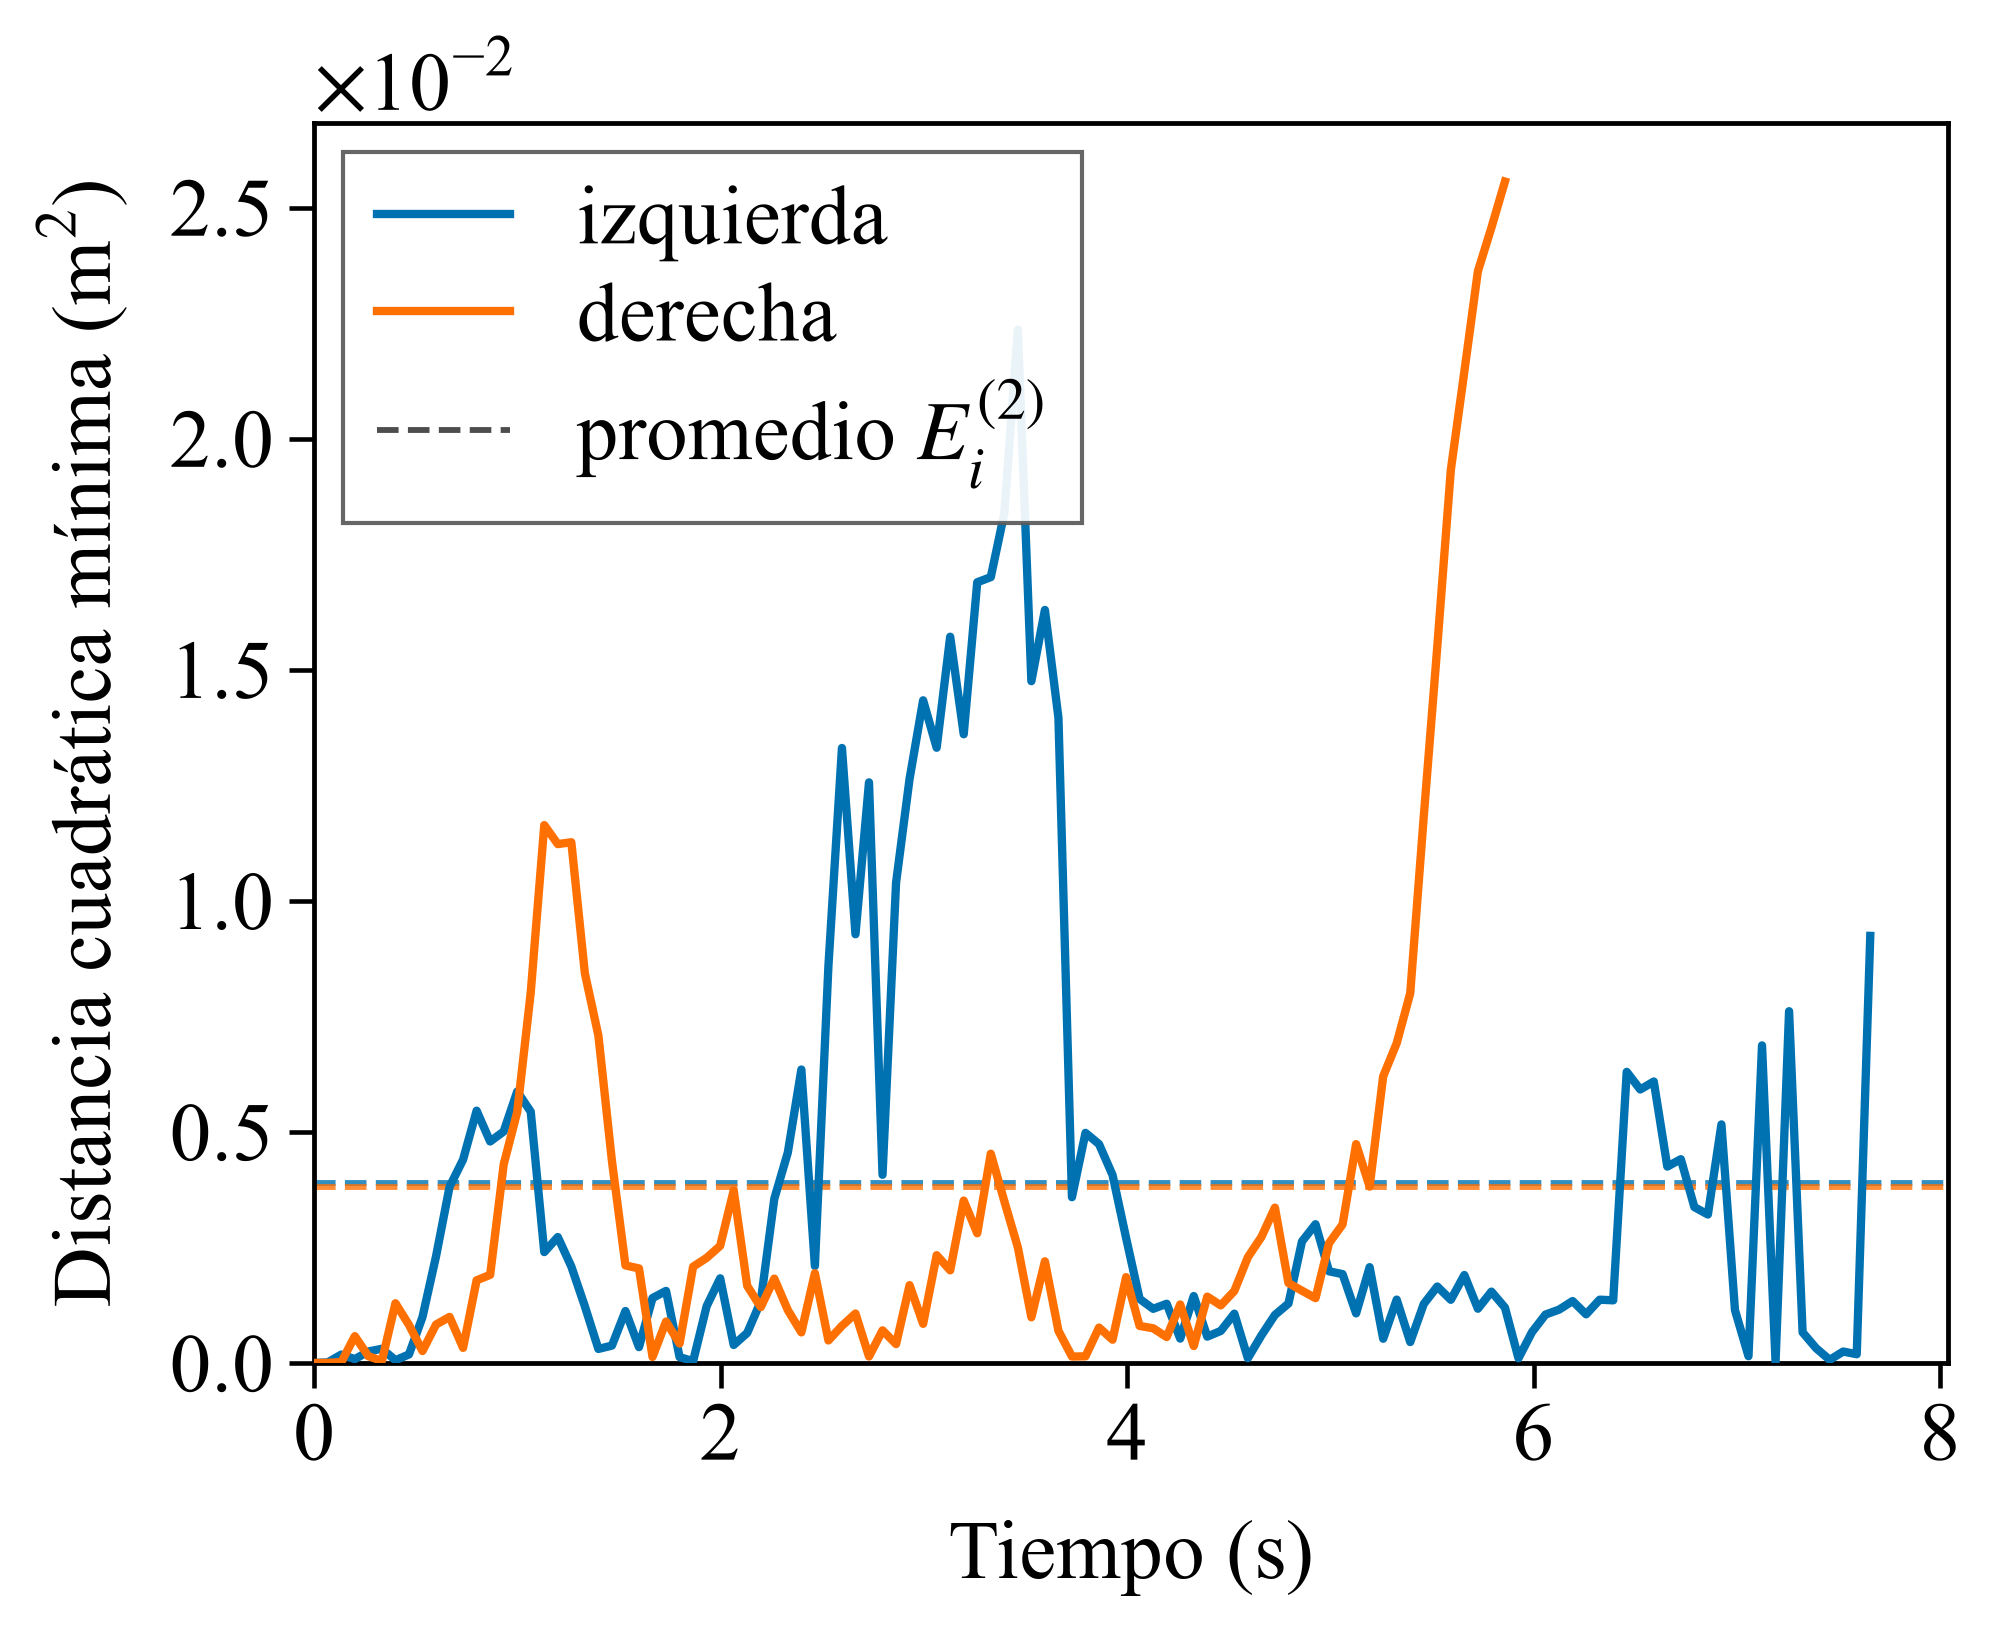
\includegraphics[width=\linewidth,height=0.60\textheight,keepaspectratio]{evol_E2_a.png}
    \end{column}
    \begin{column}{0.49\textwidth}
      \centering{\small Evento 11}\par\smallskip
      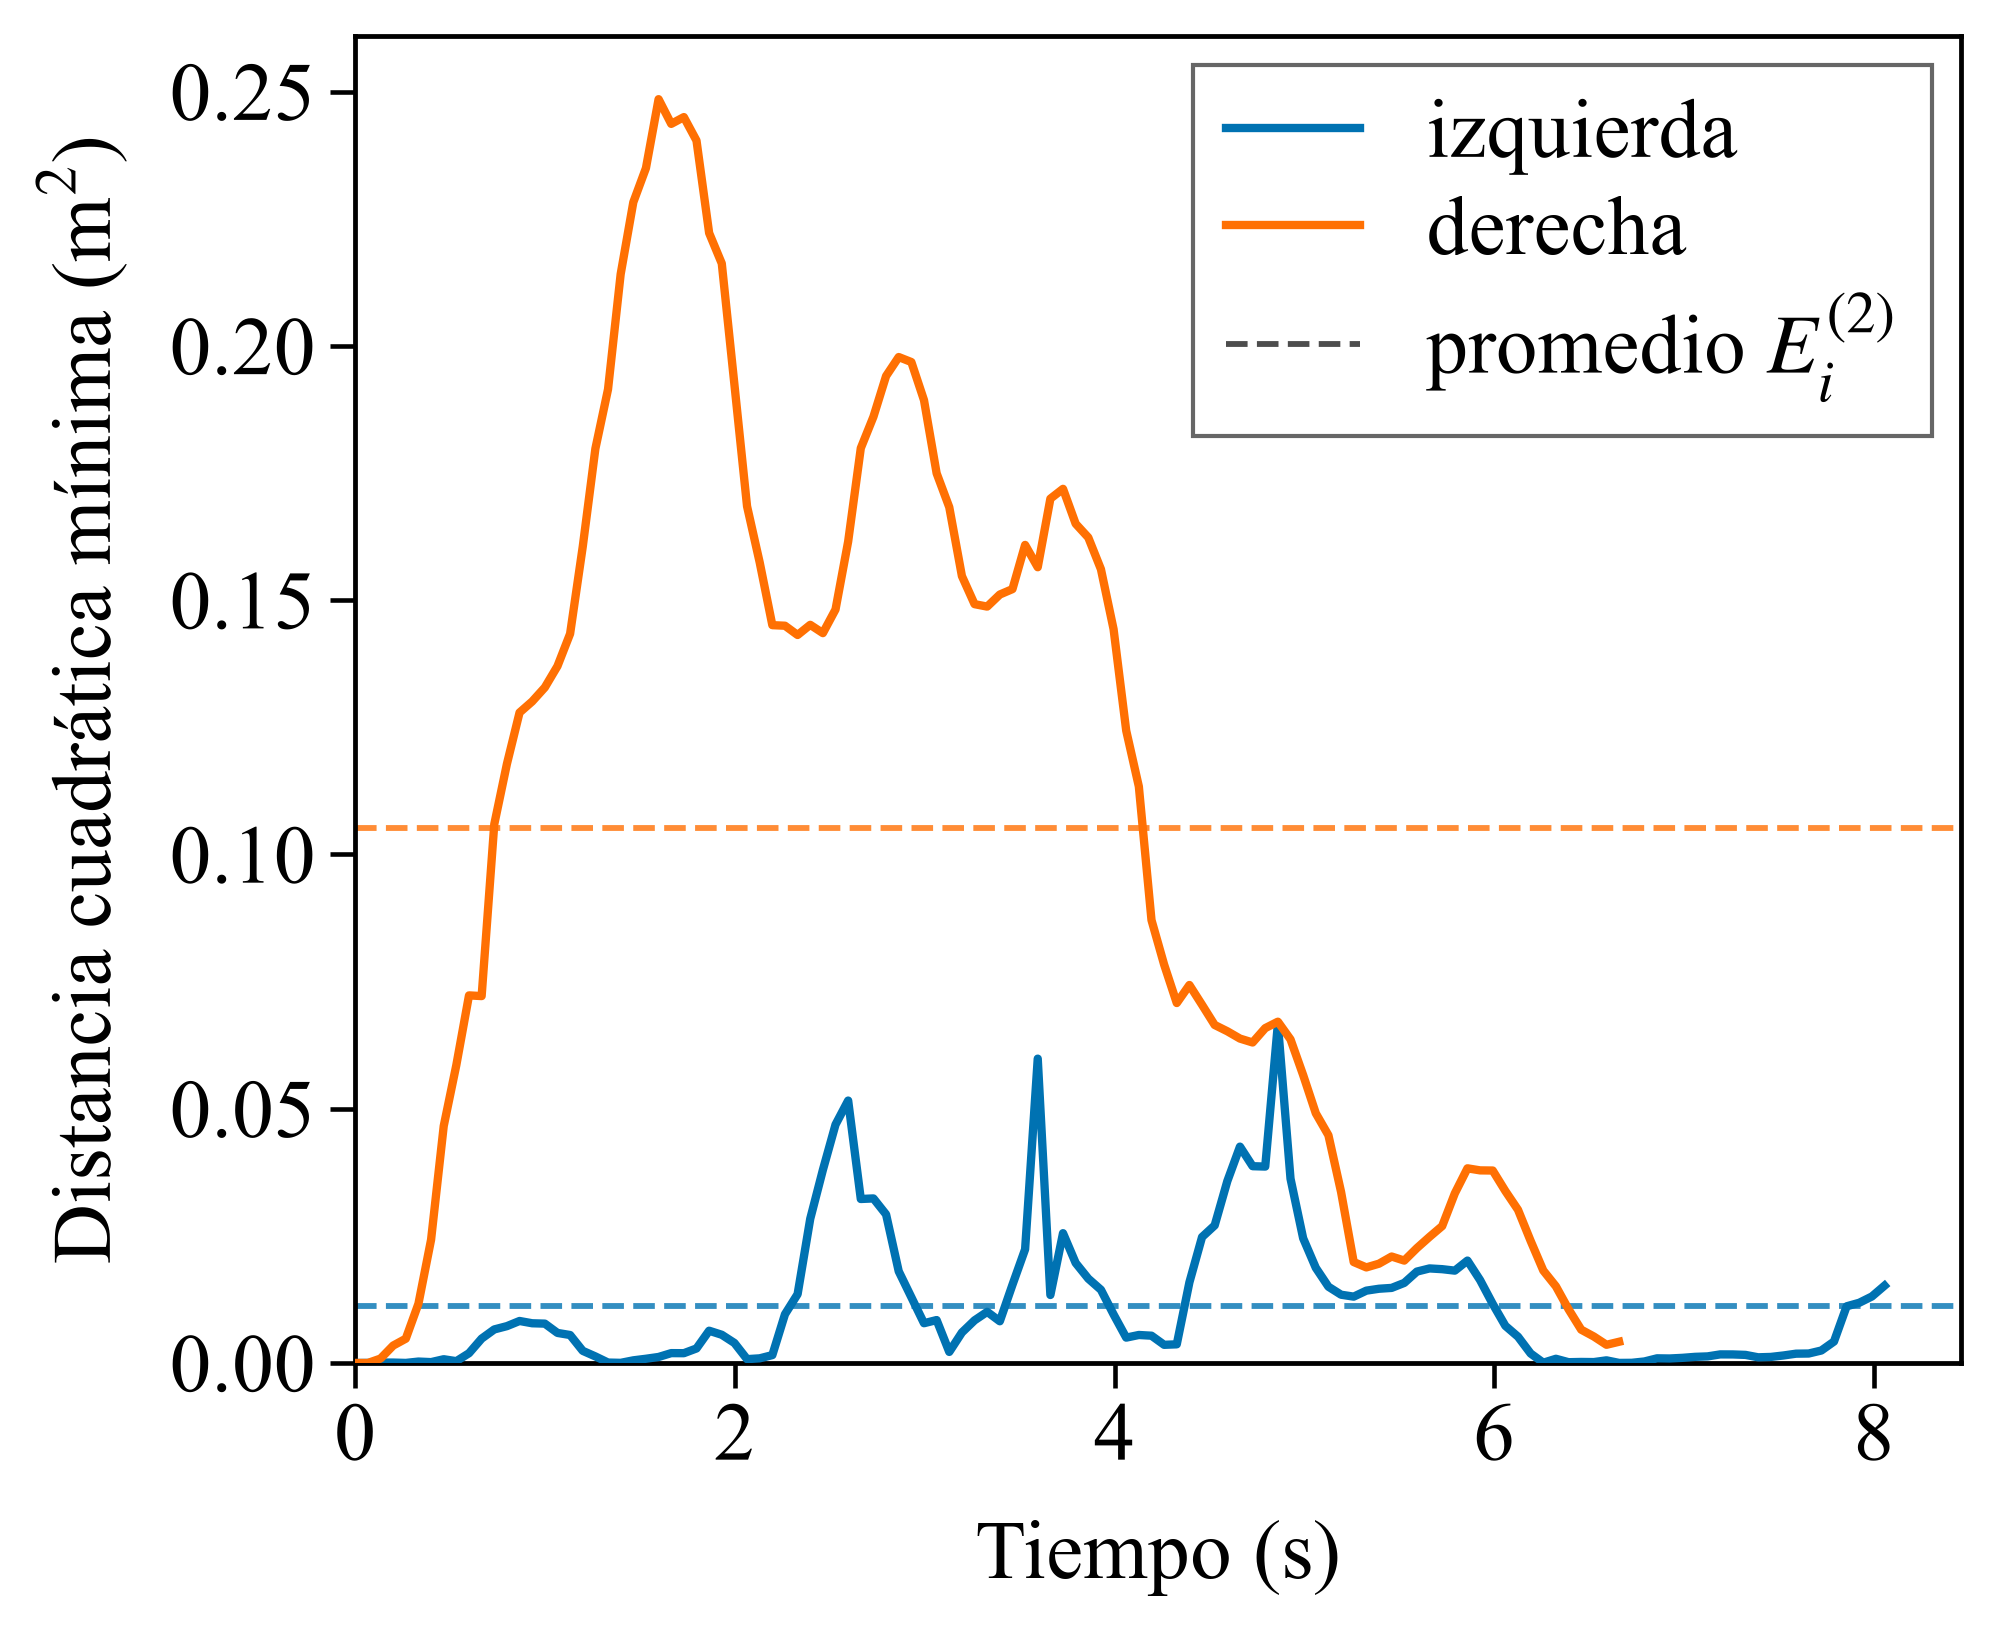
\includegraphics[width=\linewidth,height=0.60\textheight,keepaspectratio]{evol_E2_b.png}
    \end{column}
  \end{columns}
  \vspace{4pt}
  \centering{\small $d^2_{i,\min}(t_k) = \min_j\big|\vv{r}^{\,exp}_i(t_k) - \vv{r}^{\,sim}_i(t_j)\big|^2$, \quad
    punteada: $E^{(2)}_i = \frac{1}{N_m}\sum_k d^2_{i,\min}(t_k)$, \quad
    $\dlat = 0.25\uni{m}$, \ $\dact = 5\uni{m}$}
\end{frame}

\begin{frame}{Resultados}
  \framesubtitle{Calibración poblacional: métrica 1}
  \begin{cols}
    \begin{column}{0.62\textwidth}
      \figura{E1_superficie.png}
    \end{column}
    \begin{column}{0.34\textwidth}
      \begin{resultado}[Óptimo]
        \item $\dlat = 0.20\uni{m}$
        \item $\dact = 4\uni{m}$
        \item $\langle E^{(1)}\rangle = 0.4 \pm 0.3\uni{m^2}$
      \end{resultado}
    \end{column}
  \end{cols}
\end{frame}

\begin{frame}{Resultados}
  \framesubtitle{Calibración poblacional: métrica 1, cortes por el óptimo}
  \begin{columns}[T]
    \begin{column}{0.49\textwidth}
      \centering
      {\small Variando $\dlat$, con $\dact = 4\uni{m}$ fijo\par}
      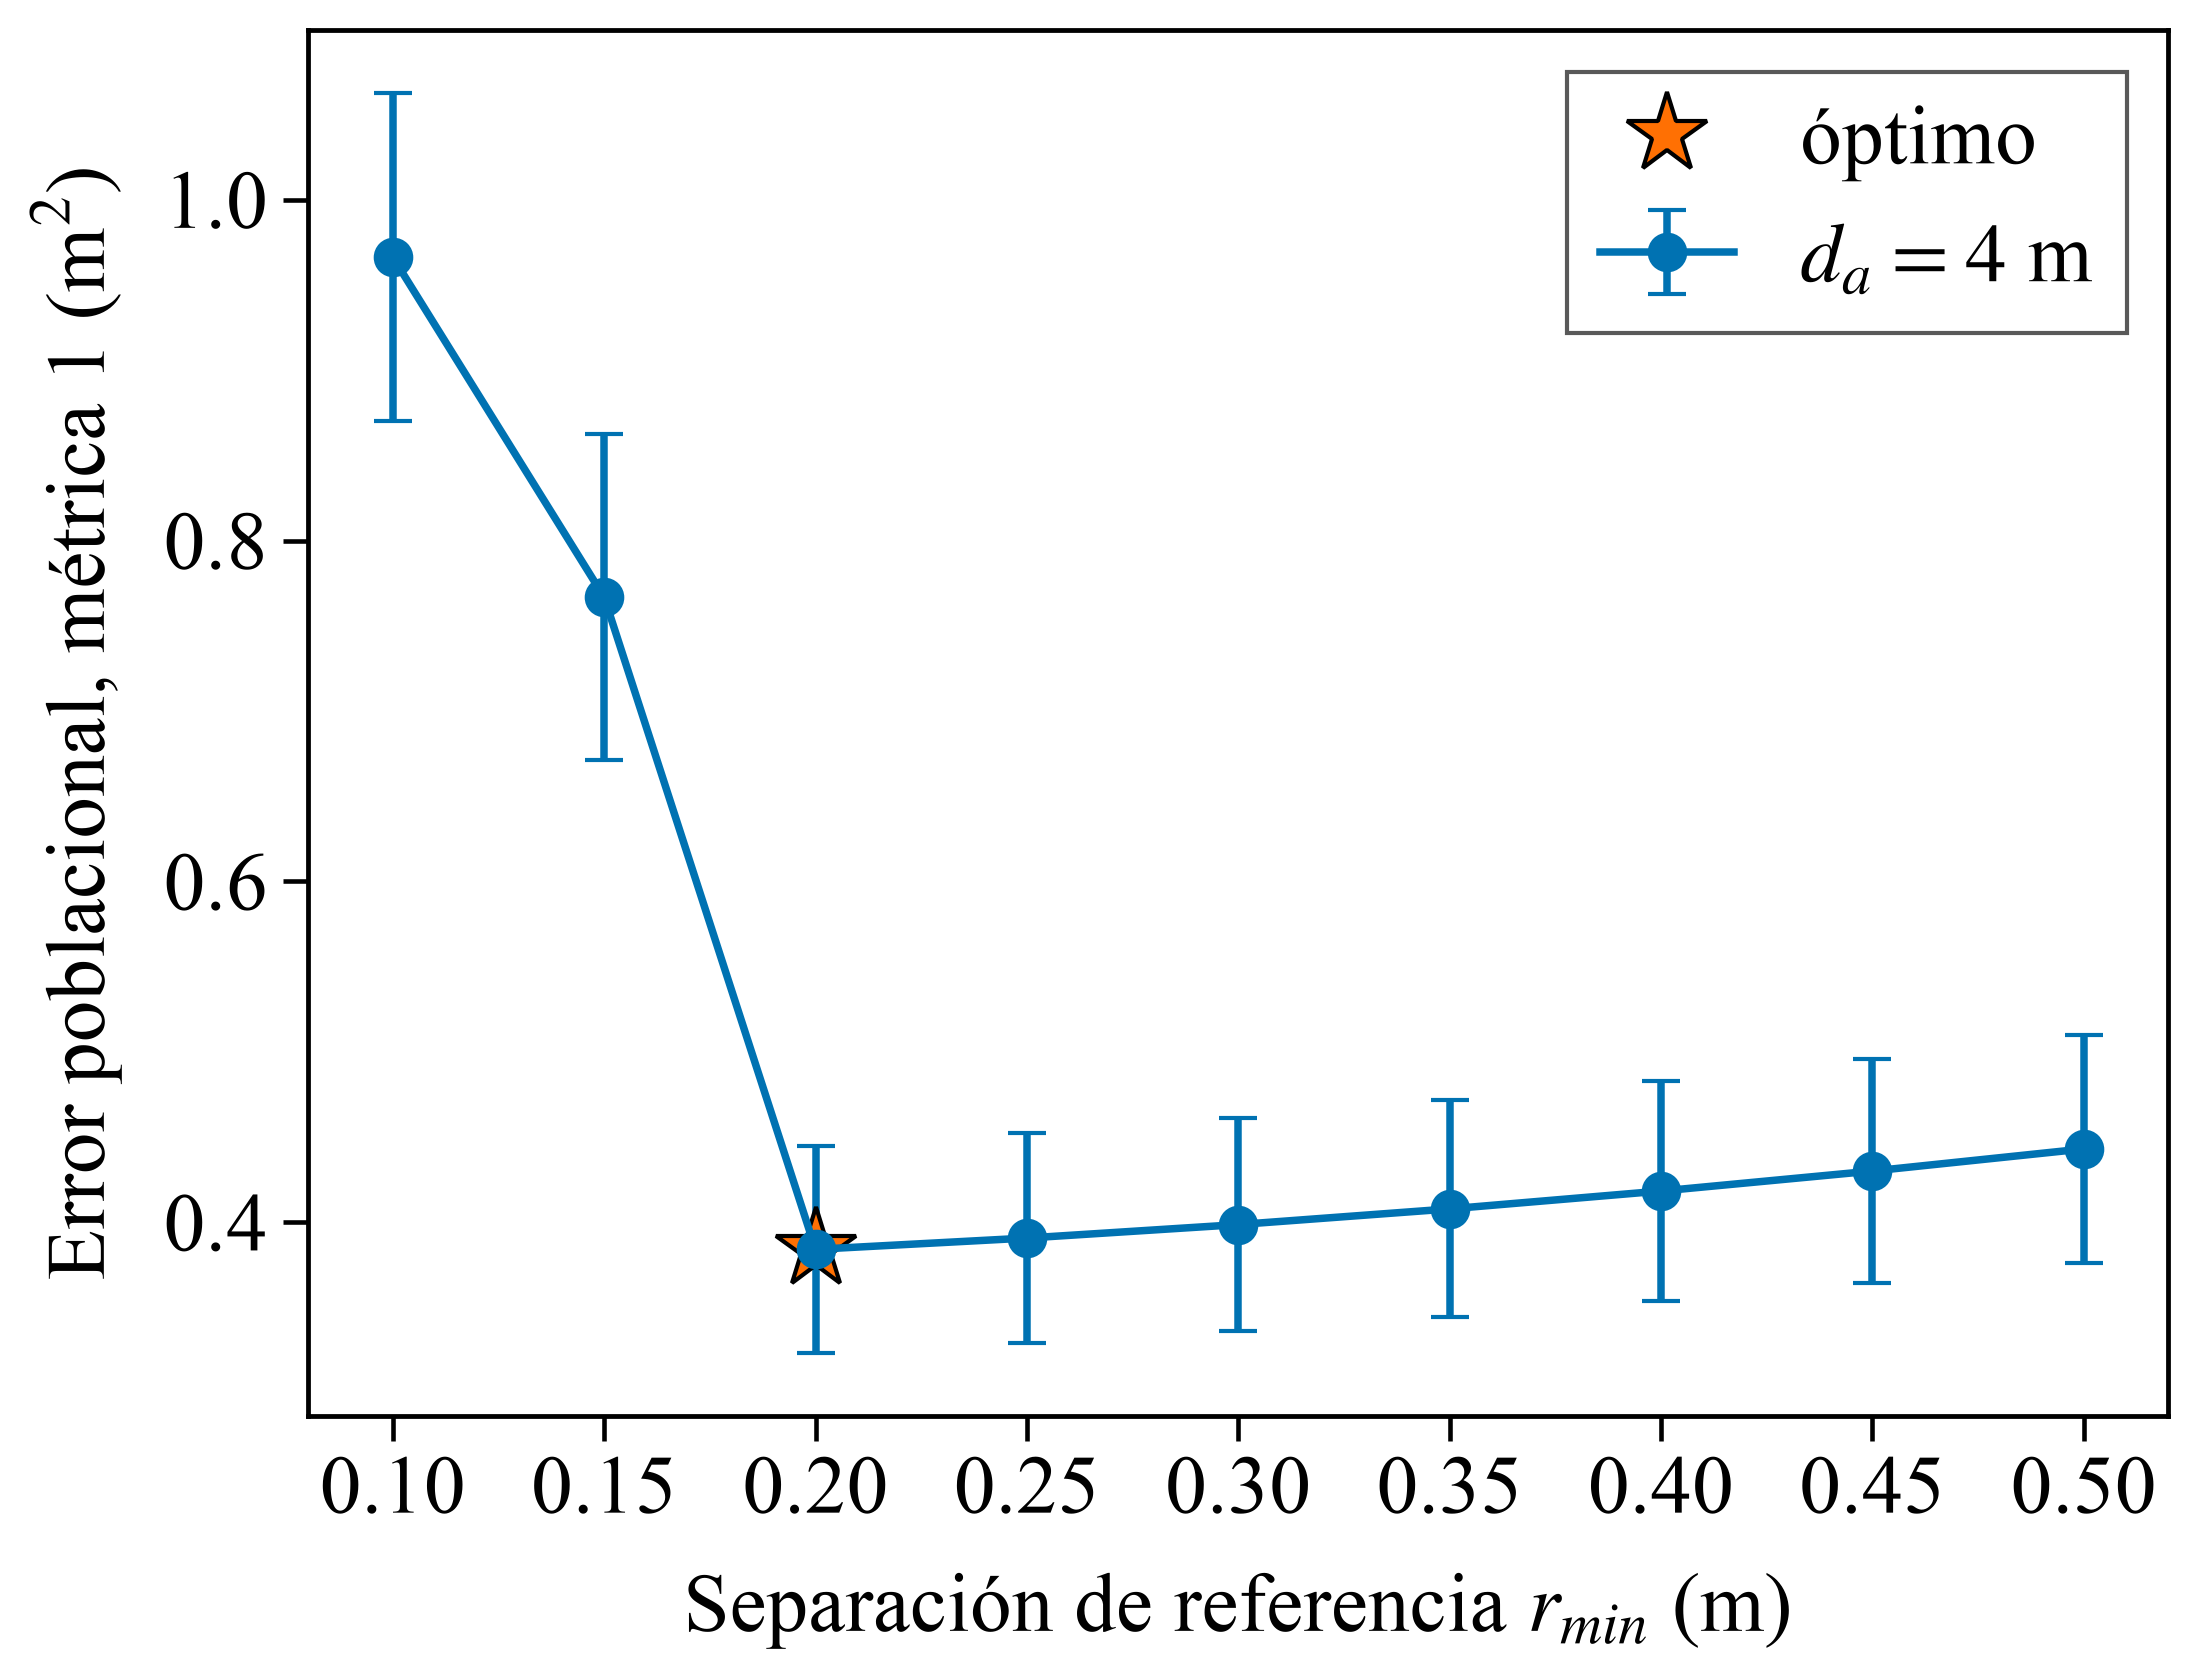
\includegraphics[width=\linewidth,height=0.62\textheight,keepaspectratio]{E1_corte_rmin.png}
    \end{column}
    \begin{column}{0.49\textwidth}
      \centering
      {\small Variando $\dact$, con $\dlat = 0.20\uni{m}$ fijo\par}
      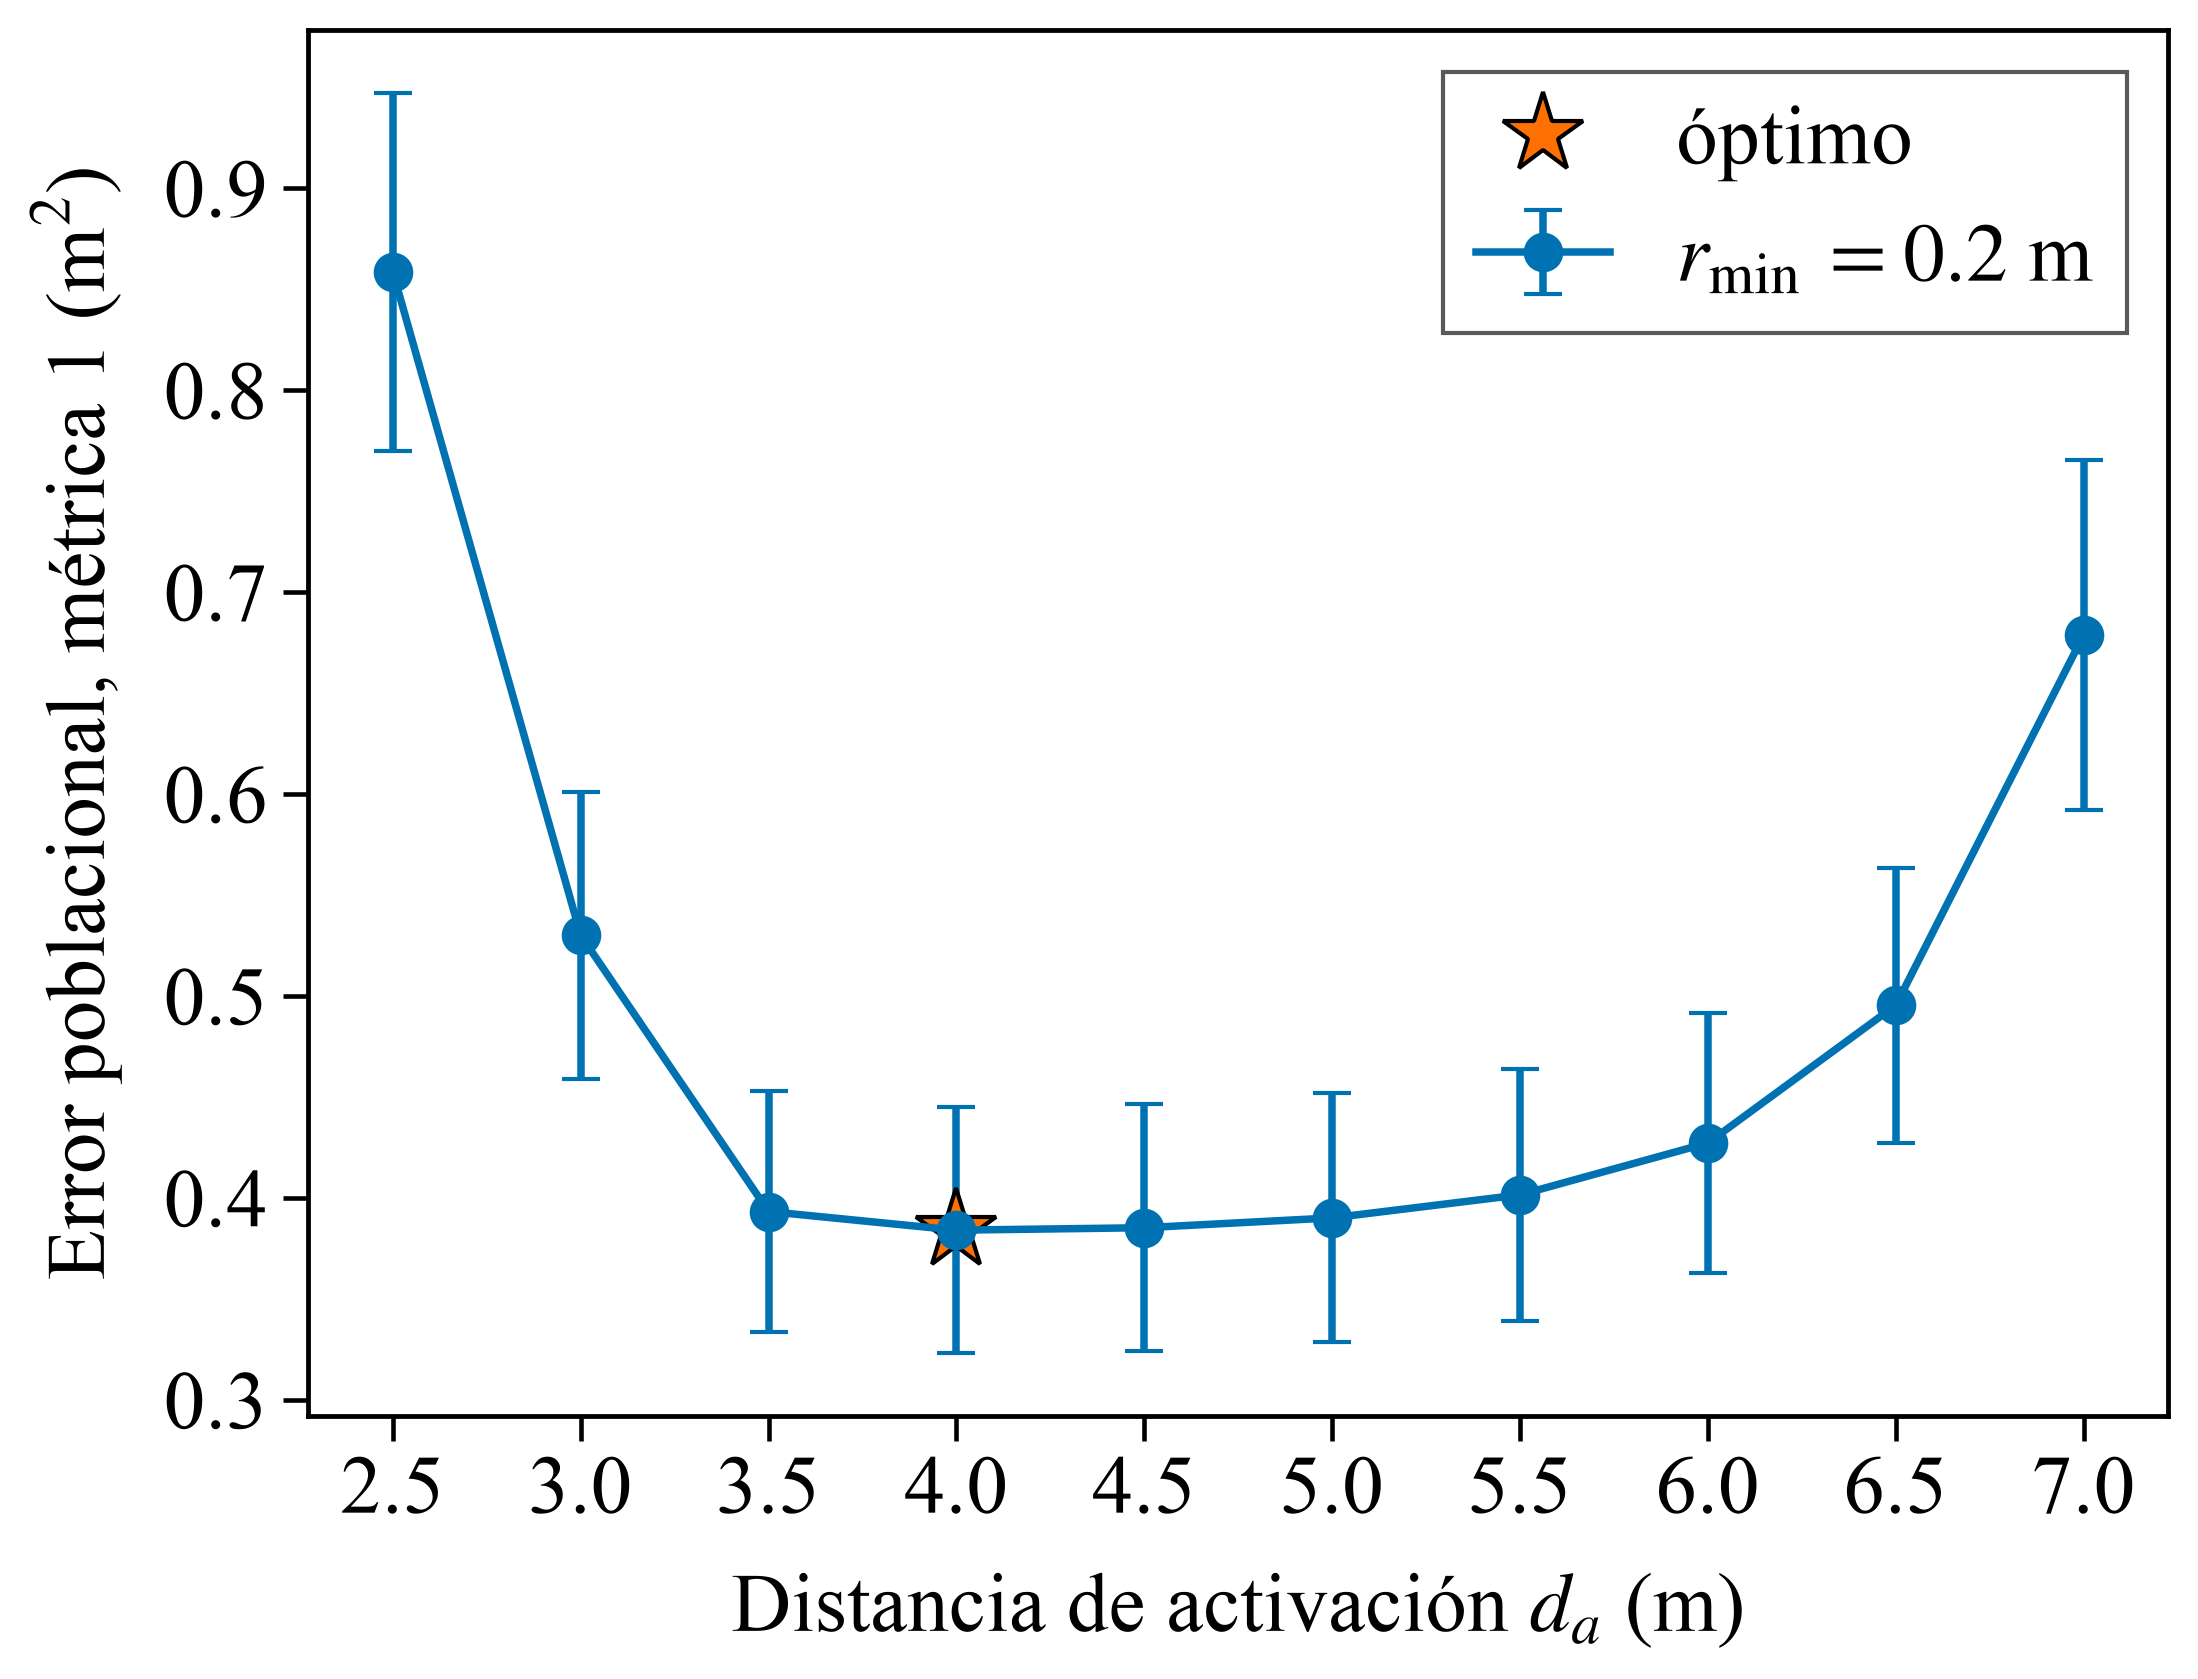
\includegraphics[width=\linewidth,height=0.62\textheight,keepaspectratio]{E1_corte_action_distance.png}
    \end{column}
  \end{columns}
\end{frame}

\begin{frame}{Resultados}
  \framesubtitle{Calibración poblacional: métrica 2}
  \begin{cols}
    \begin{column}{0.62\textwidth}
      \figura{E2_superficie.png}
    \end{column}
    \begin{column}{0.34\textwidth}
      \begin{resultado}[Óptimo]
        \item $\dlat = 0.25\uni{m}$
        \item $\dact = 5\uni{m}$
        \item $\langle E^{(2)}\rangle = (2 \pm 1)\ten{-2}\uni{m^2}$
      \end{resultado}
    \end{column}
  \end{cols}
\end{frame}

\begin{frame}{Resultados}
  \framesubtitle{Calibración poblacional: métrica 2, cortes por el óptimo}
  \begin{columns}[T]
    \begin{column}{0.49\textwidth}
      \centering
      {\small Variando $\dlat$, con $\dact = 5\uni{m}$ fijo\par}
      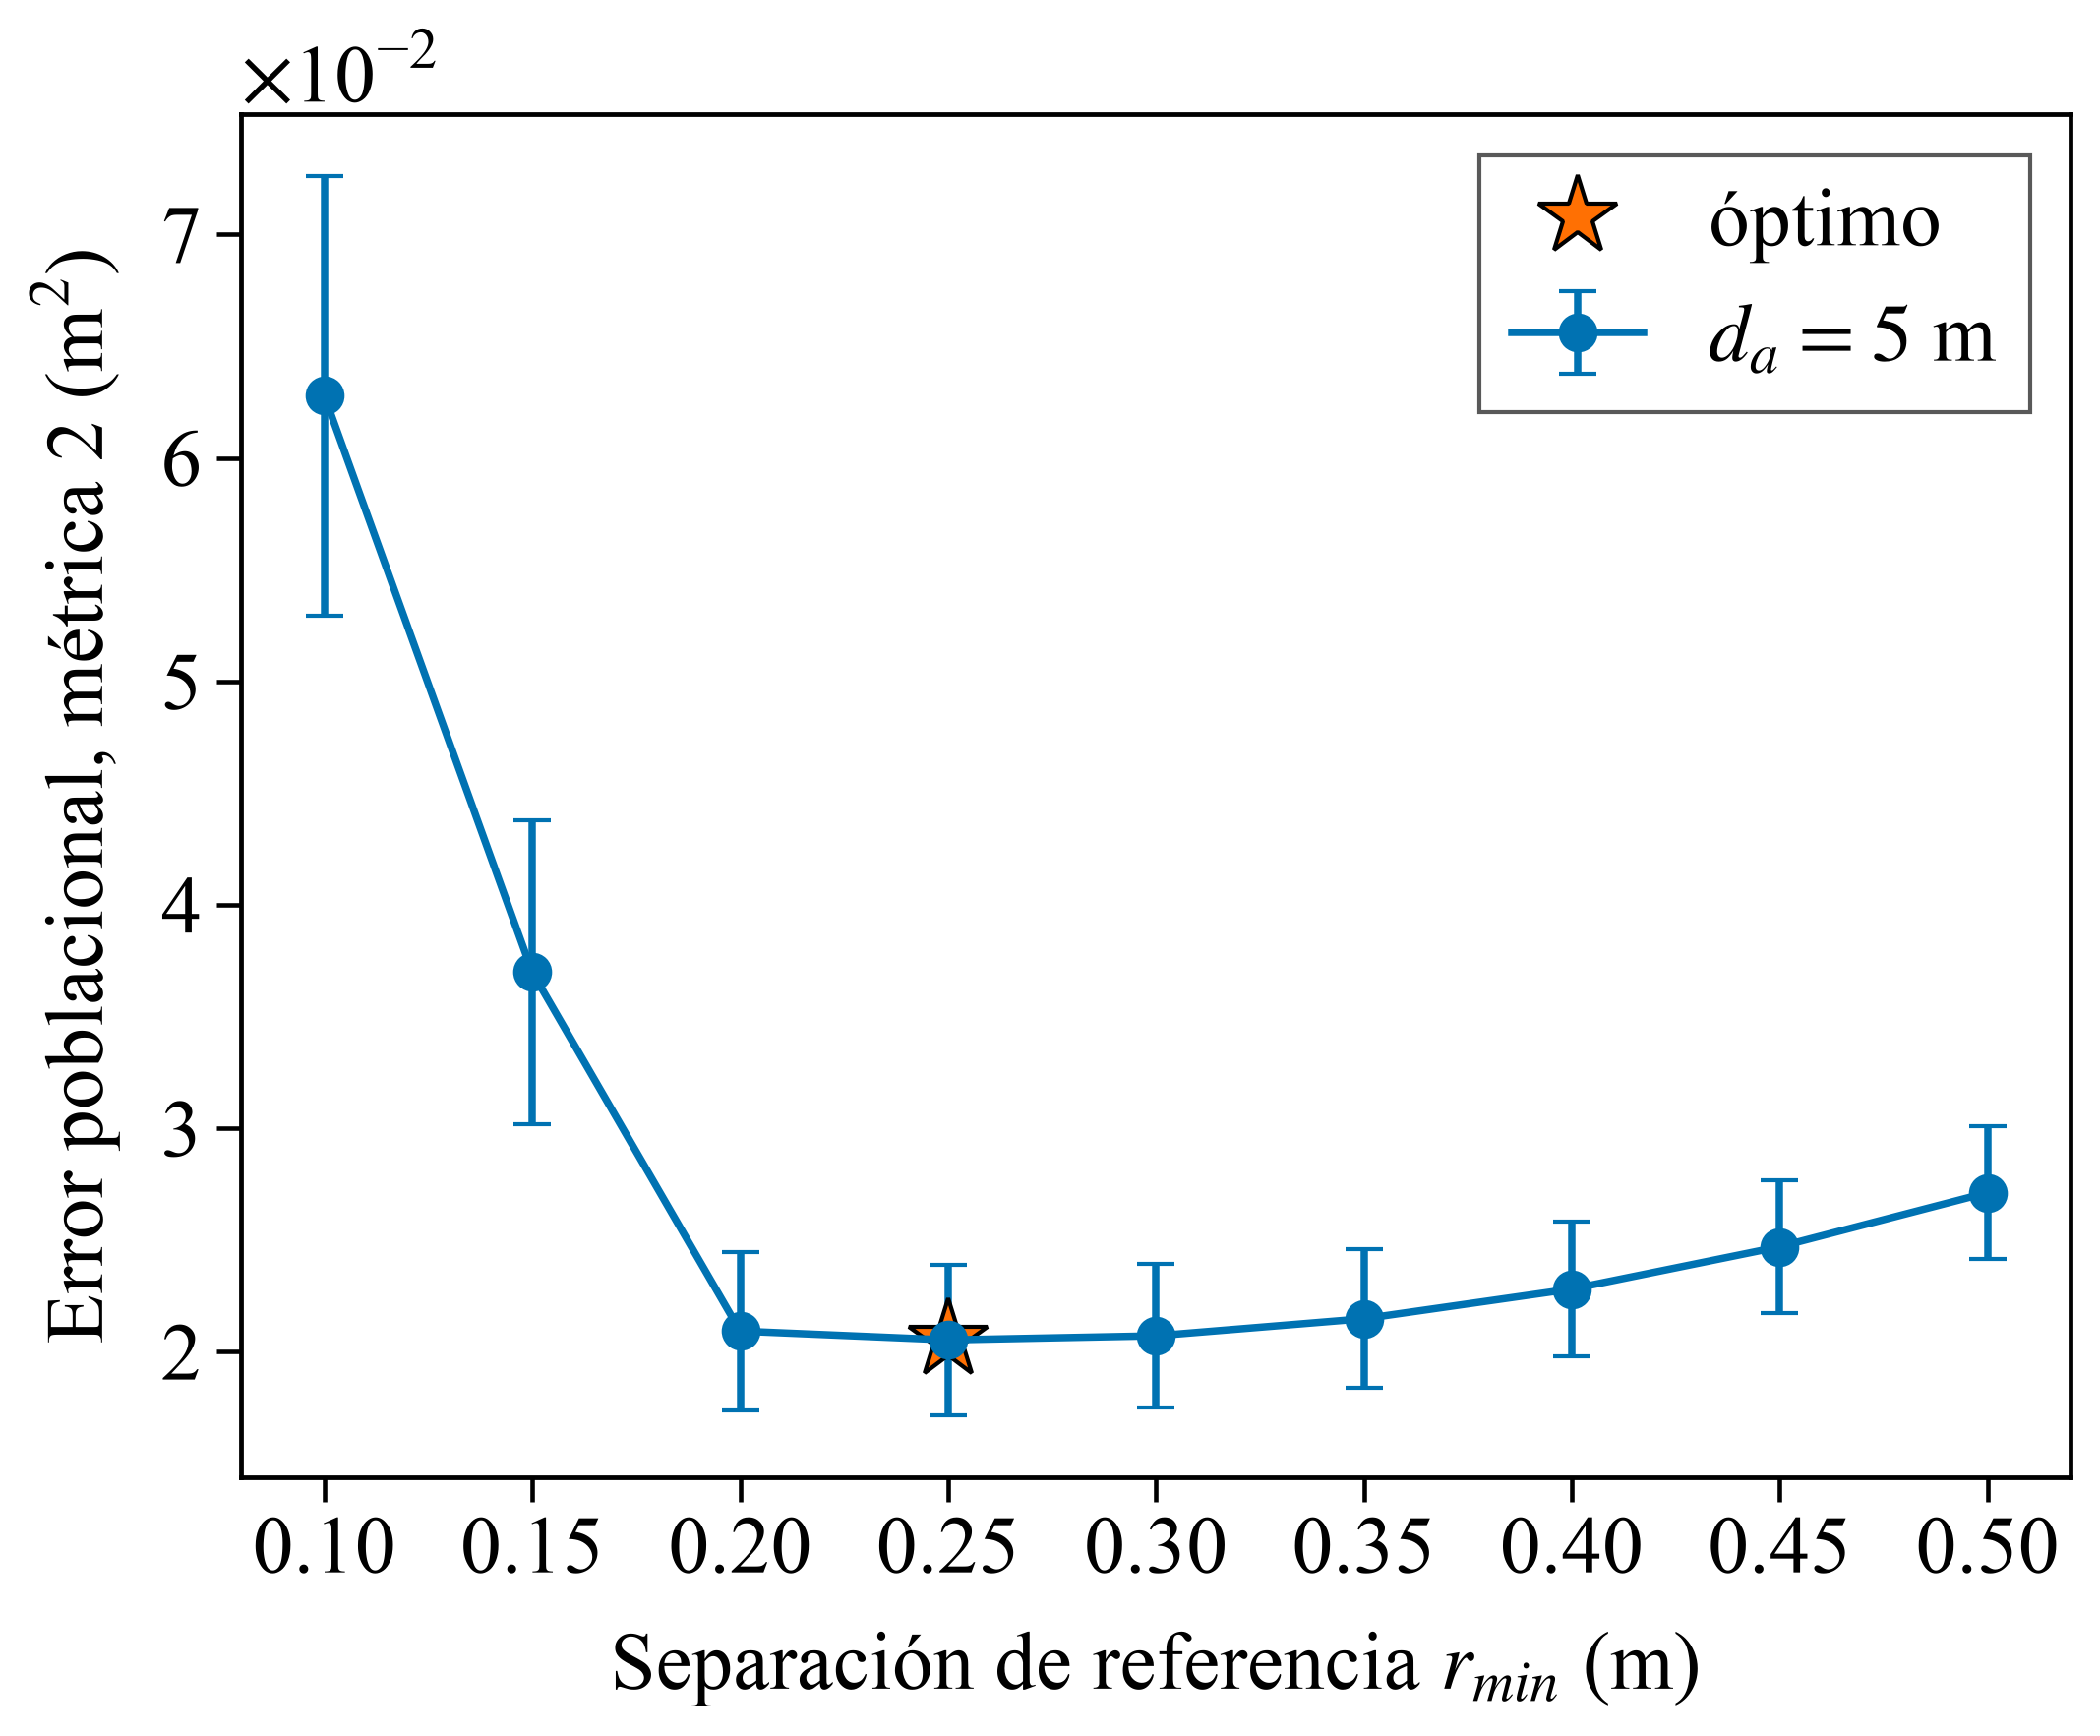
\includegraphics[width=\linewidth,height=0.62\textheight,keepaspectratio]{E2_corte_rmin.png}
    \end{column}
    \begin{column}{0.49\textwidth}
      \centering
      {\small Variando $\dact$, con $\dlat = 0.25\uni{m}$ fijo\par}
      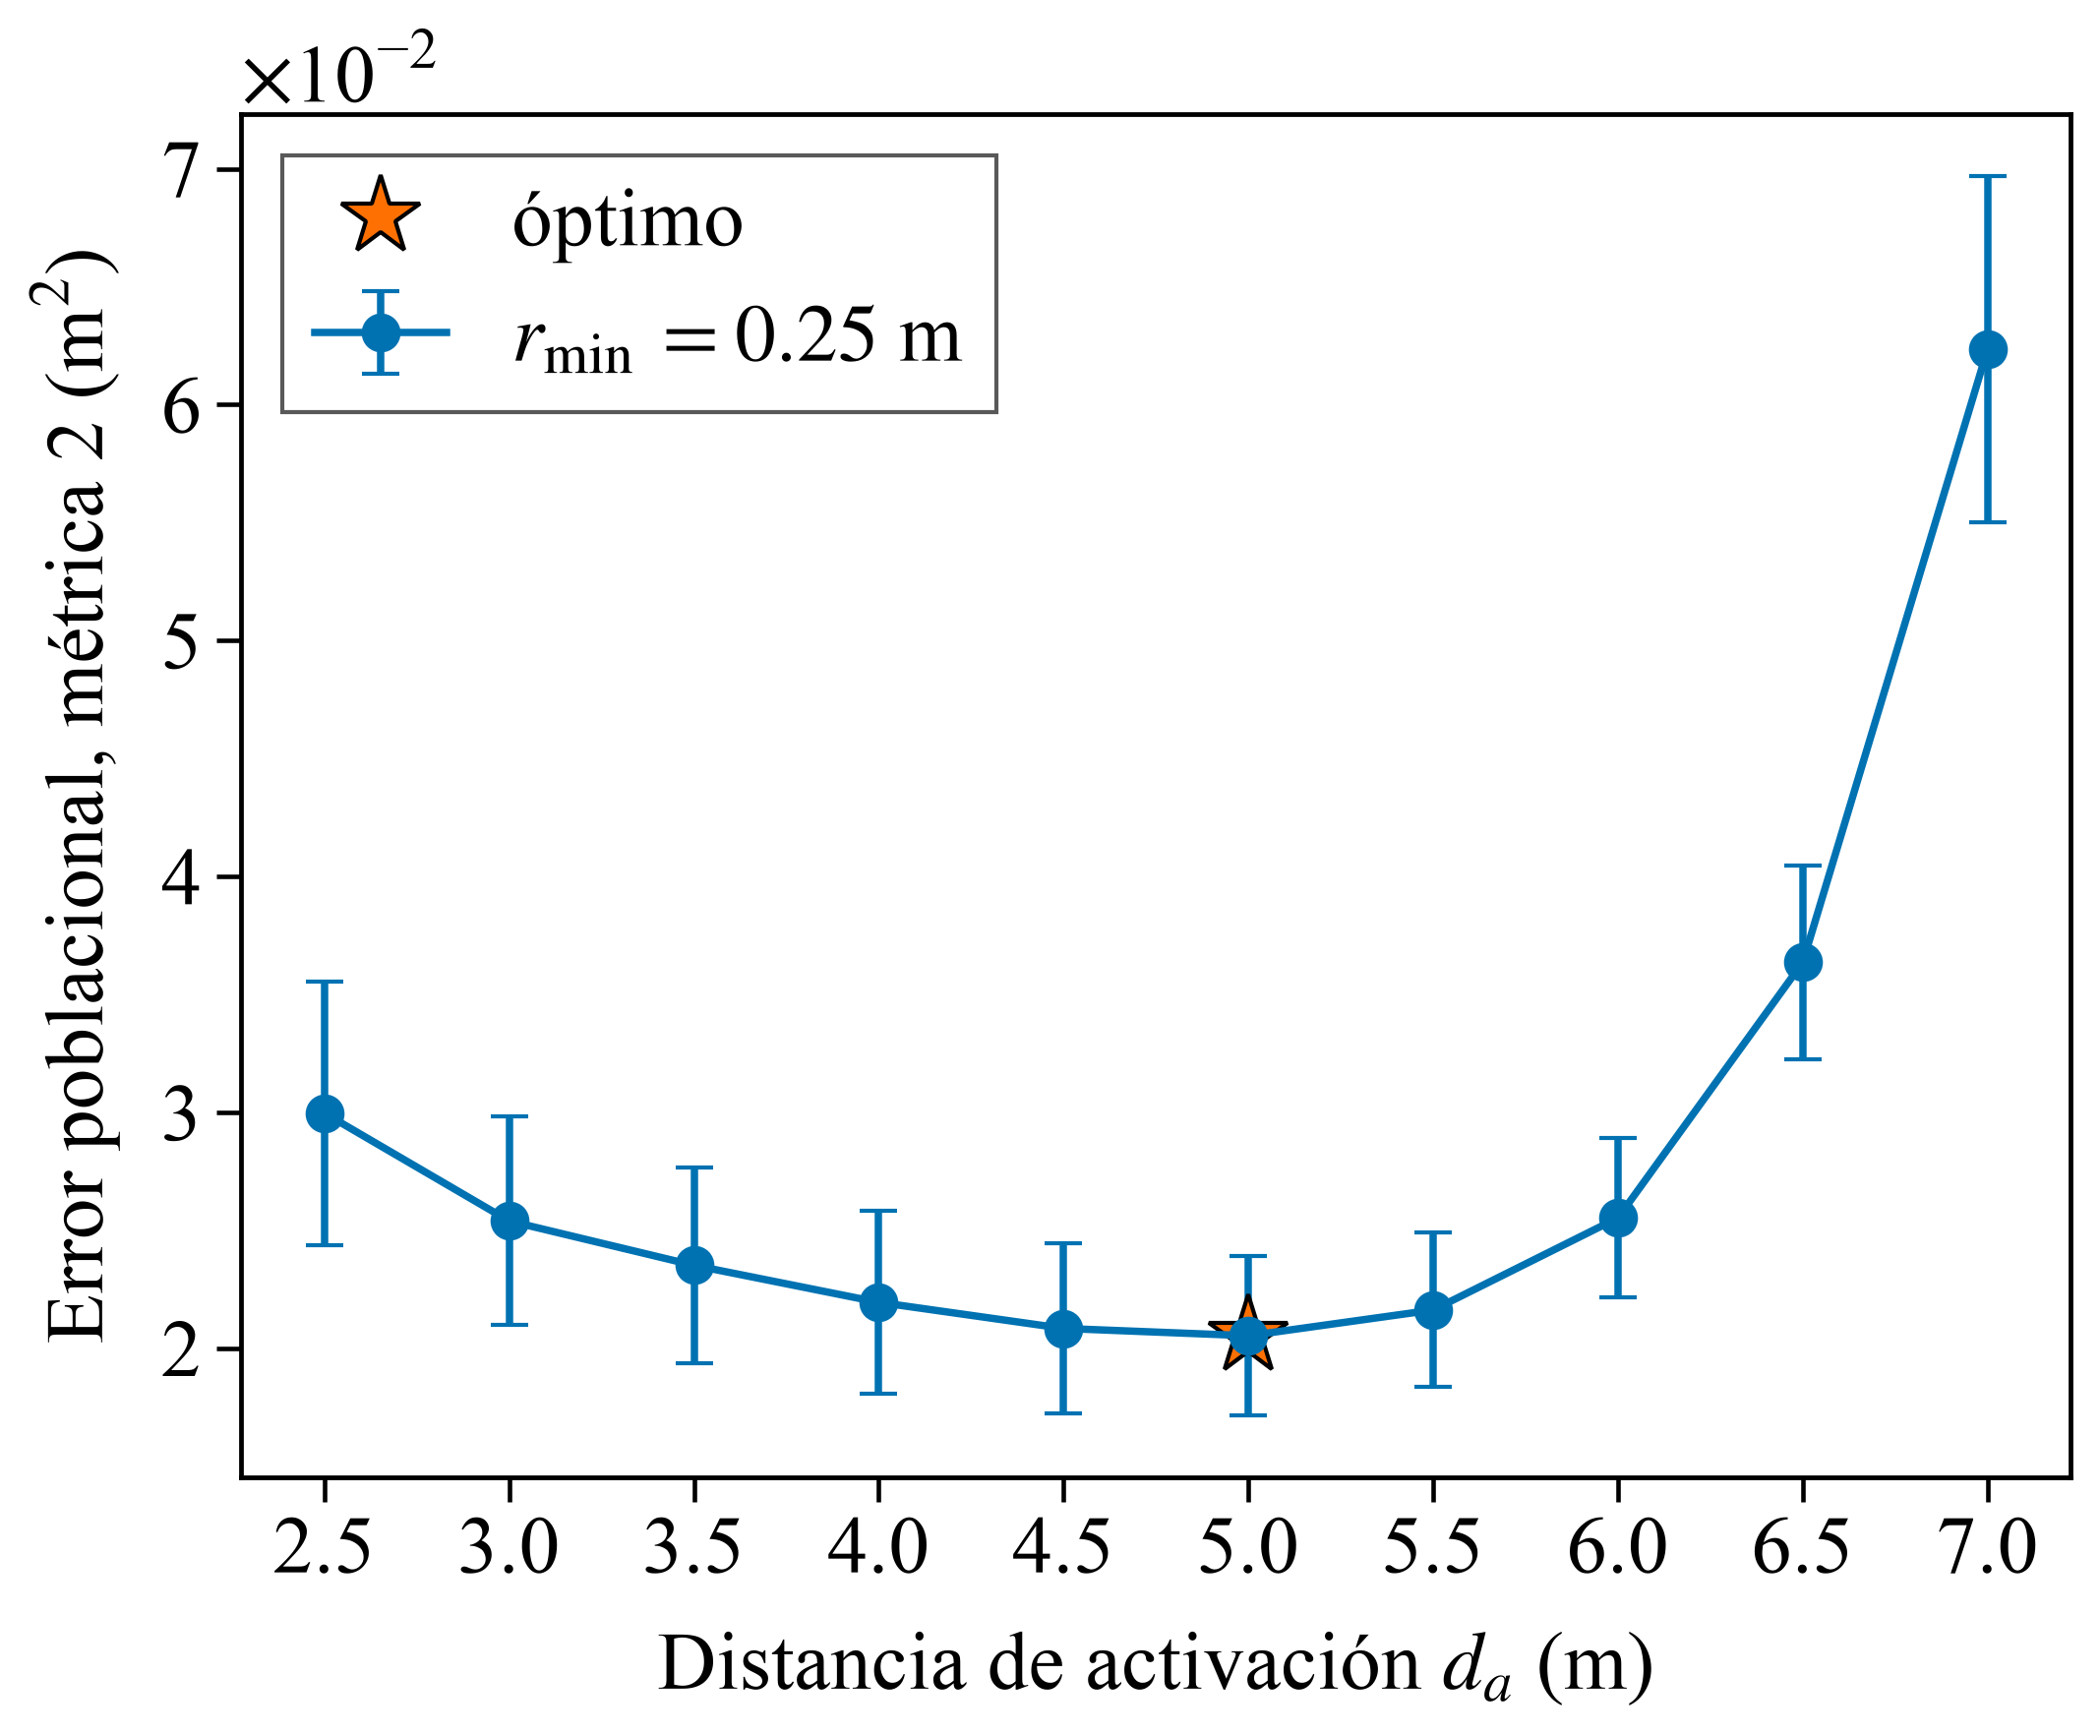
\includegraphics[width=\linewidth,height=0.62\textheight,keepaspectratio]{E2_corte_action_distance.png}
    \end{column}
  \end{columns}
\end{frame}

\begin{frame}{Resultados}
  \framesubtitle{Calibración poblacional: comparación de los óptimos}
  \centering
  \renewcommand{\arraystretch}{1.5}
  \begin{tabular}{lccc}
    \hline
    Métrica & $\dlat$ (m) & $\dact$ (m) & $\langle E\rangle$ (m$^2$) \\
    \hline
    1: iguales tiempos & $0.20$ & $4$ & $0.4 \pm 0.3$ \\
    2: punto más cercano & $0.25$ & $5$ & $(2 \pm 1)\ten{-2}$ \\
    \hline
  \end{tabular}

  \vspace{16pt}
  \begin{columns}
    \begin{column}{0.62\textwidth}
      \begin{resultado}
        \item Óptimos a un paso de grilla entre sí
        \item $\langle E^{(1)}\rangle \approx 19\,\langle E^{(2)}\rangle$
        \item $\sqrt{\langle E\rangle}$: $0.62\uni{m}$ (métrica 1), $0.14\uni{m}$ (métrica 2)
      \end{resultado}
    \end{column}
  \end{columns}
\end{frame}

\begin{frame}{Resultados}
  \framesubtitle{Calibración individual: óptimos de cada evento}
  \begin{columns}[T]
    \begin{column}{0.49\textwidth}
      \centering{\small Métrica 1}\par
      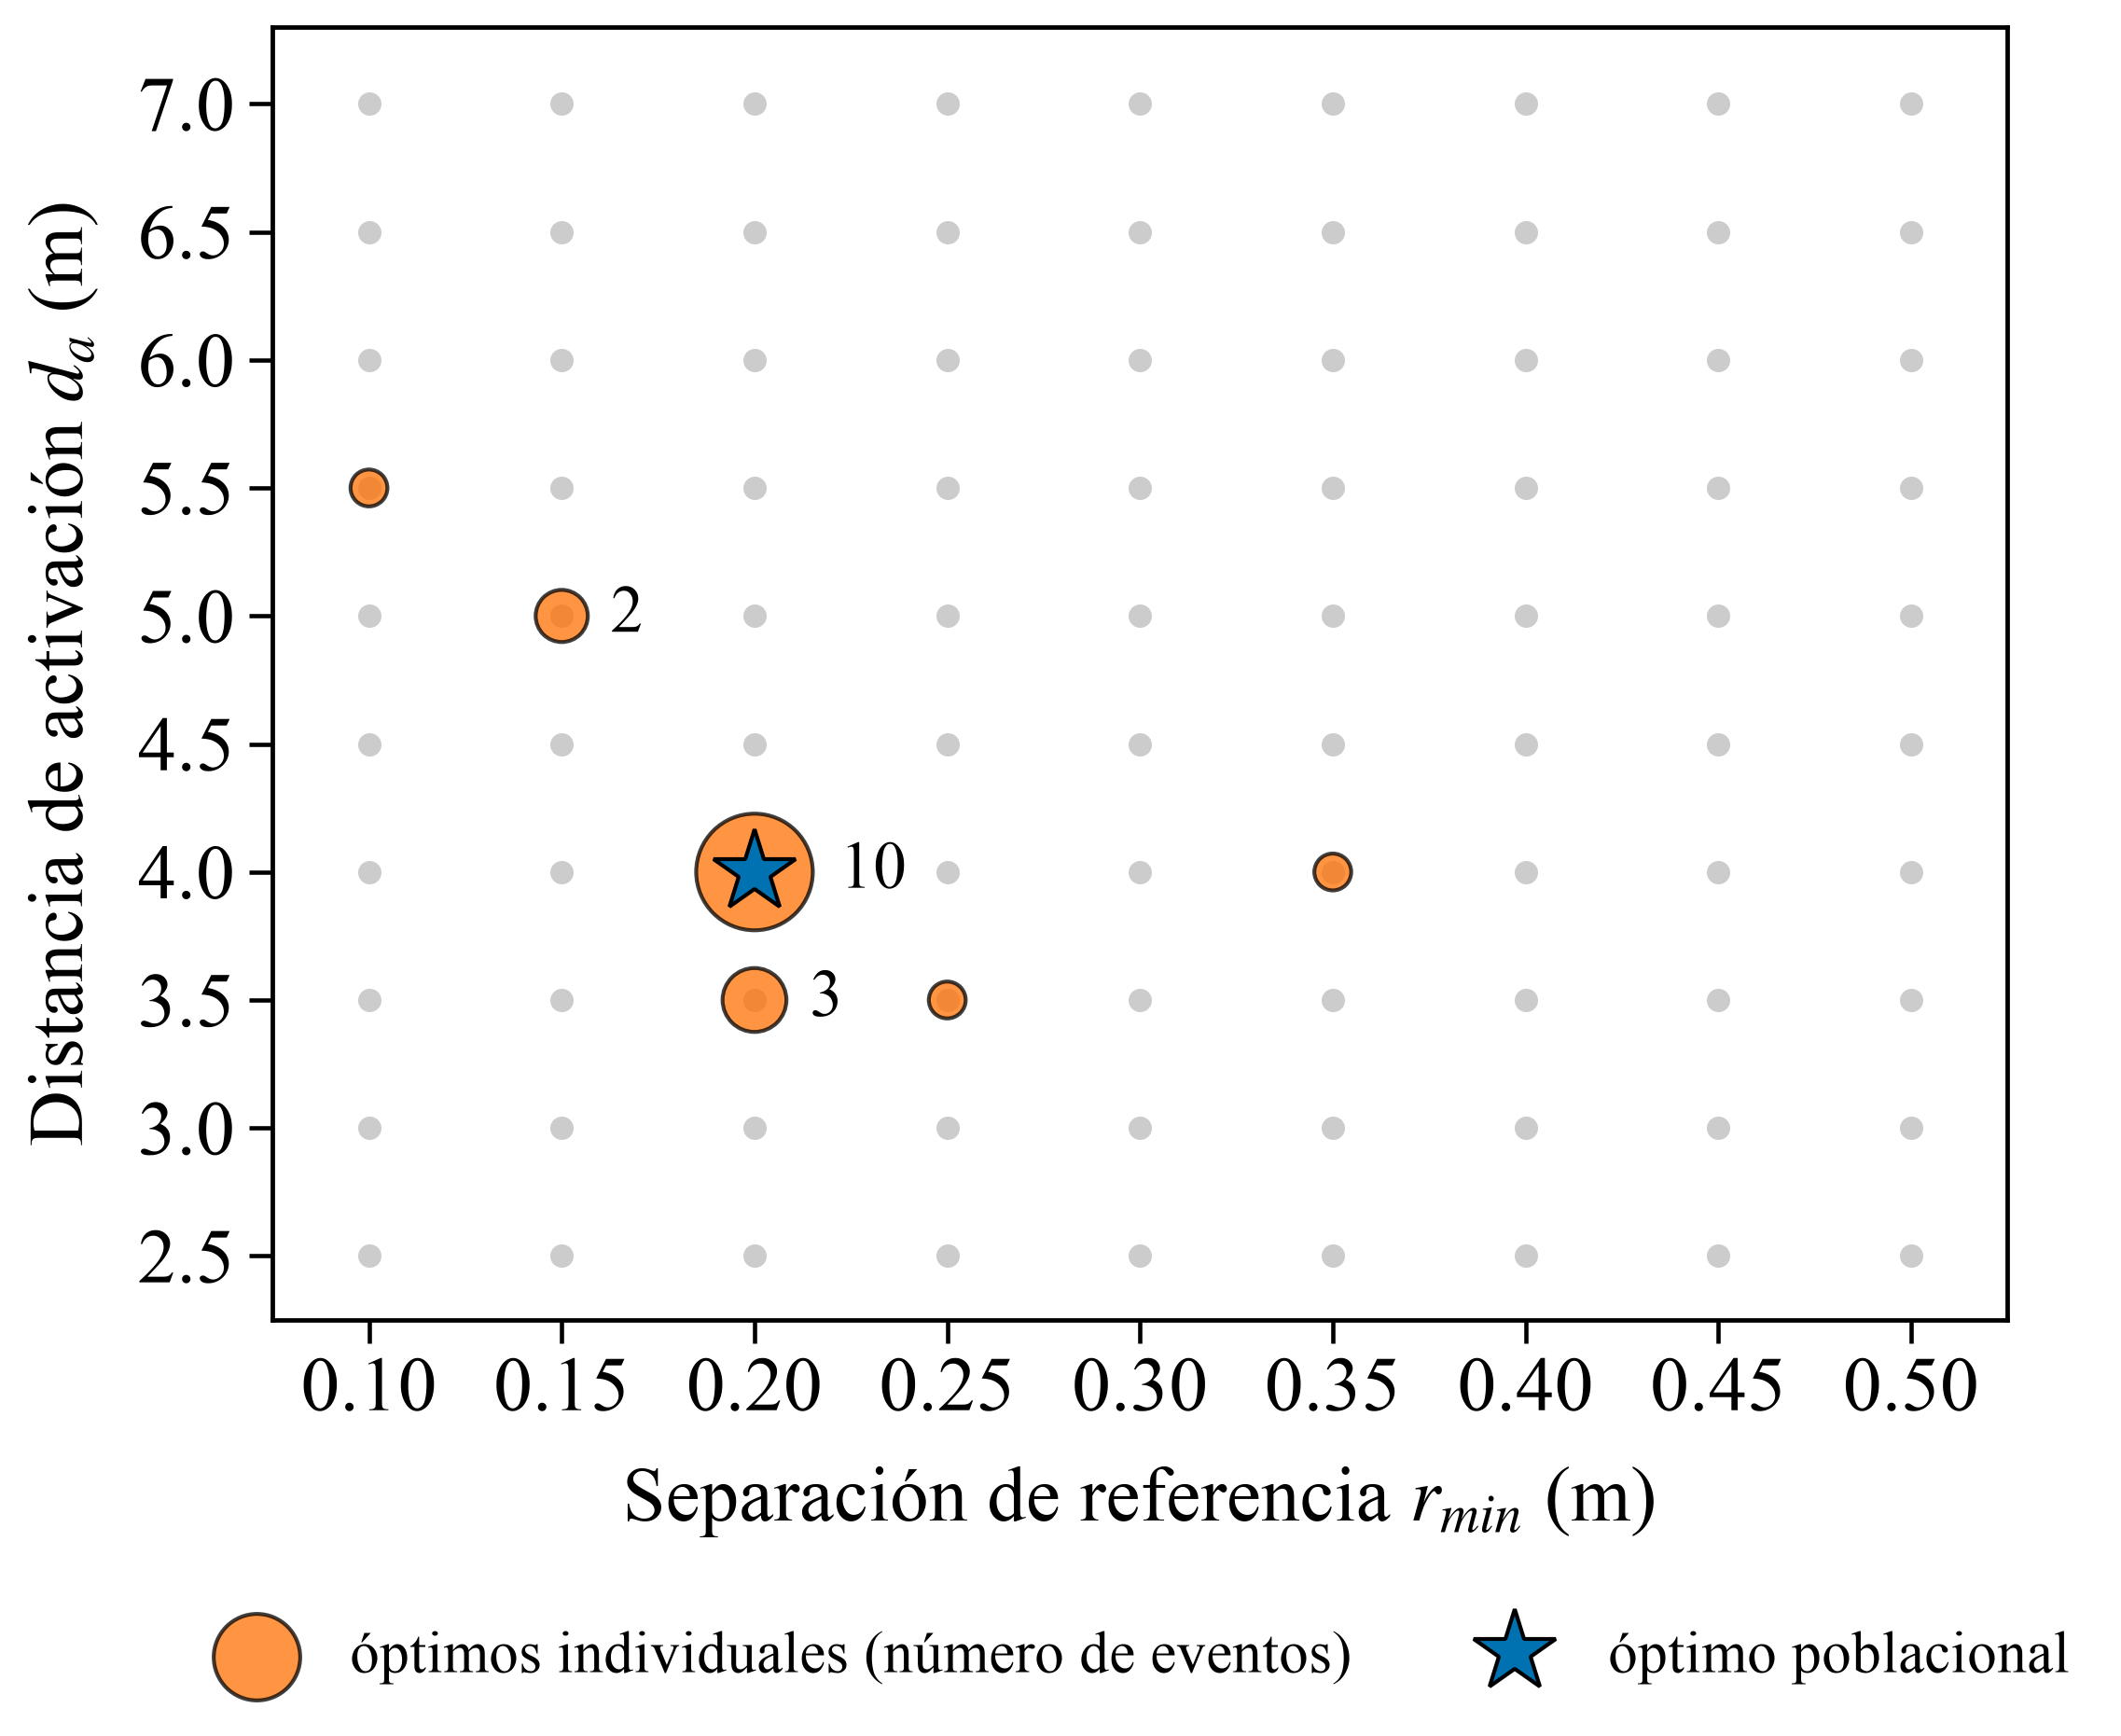
\includegraphics[width=\linewidth,height=0.70\textheight,keepaspectratio]{E1_optimos_individuales.png}
    \end{column}
    \begin{column}{0.49\textwidth}
      \centering{\small Métrica 2}\par
      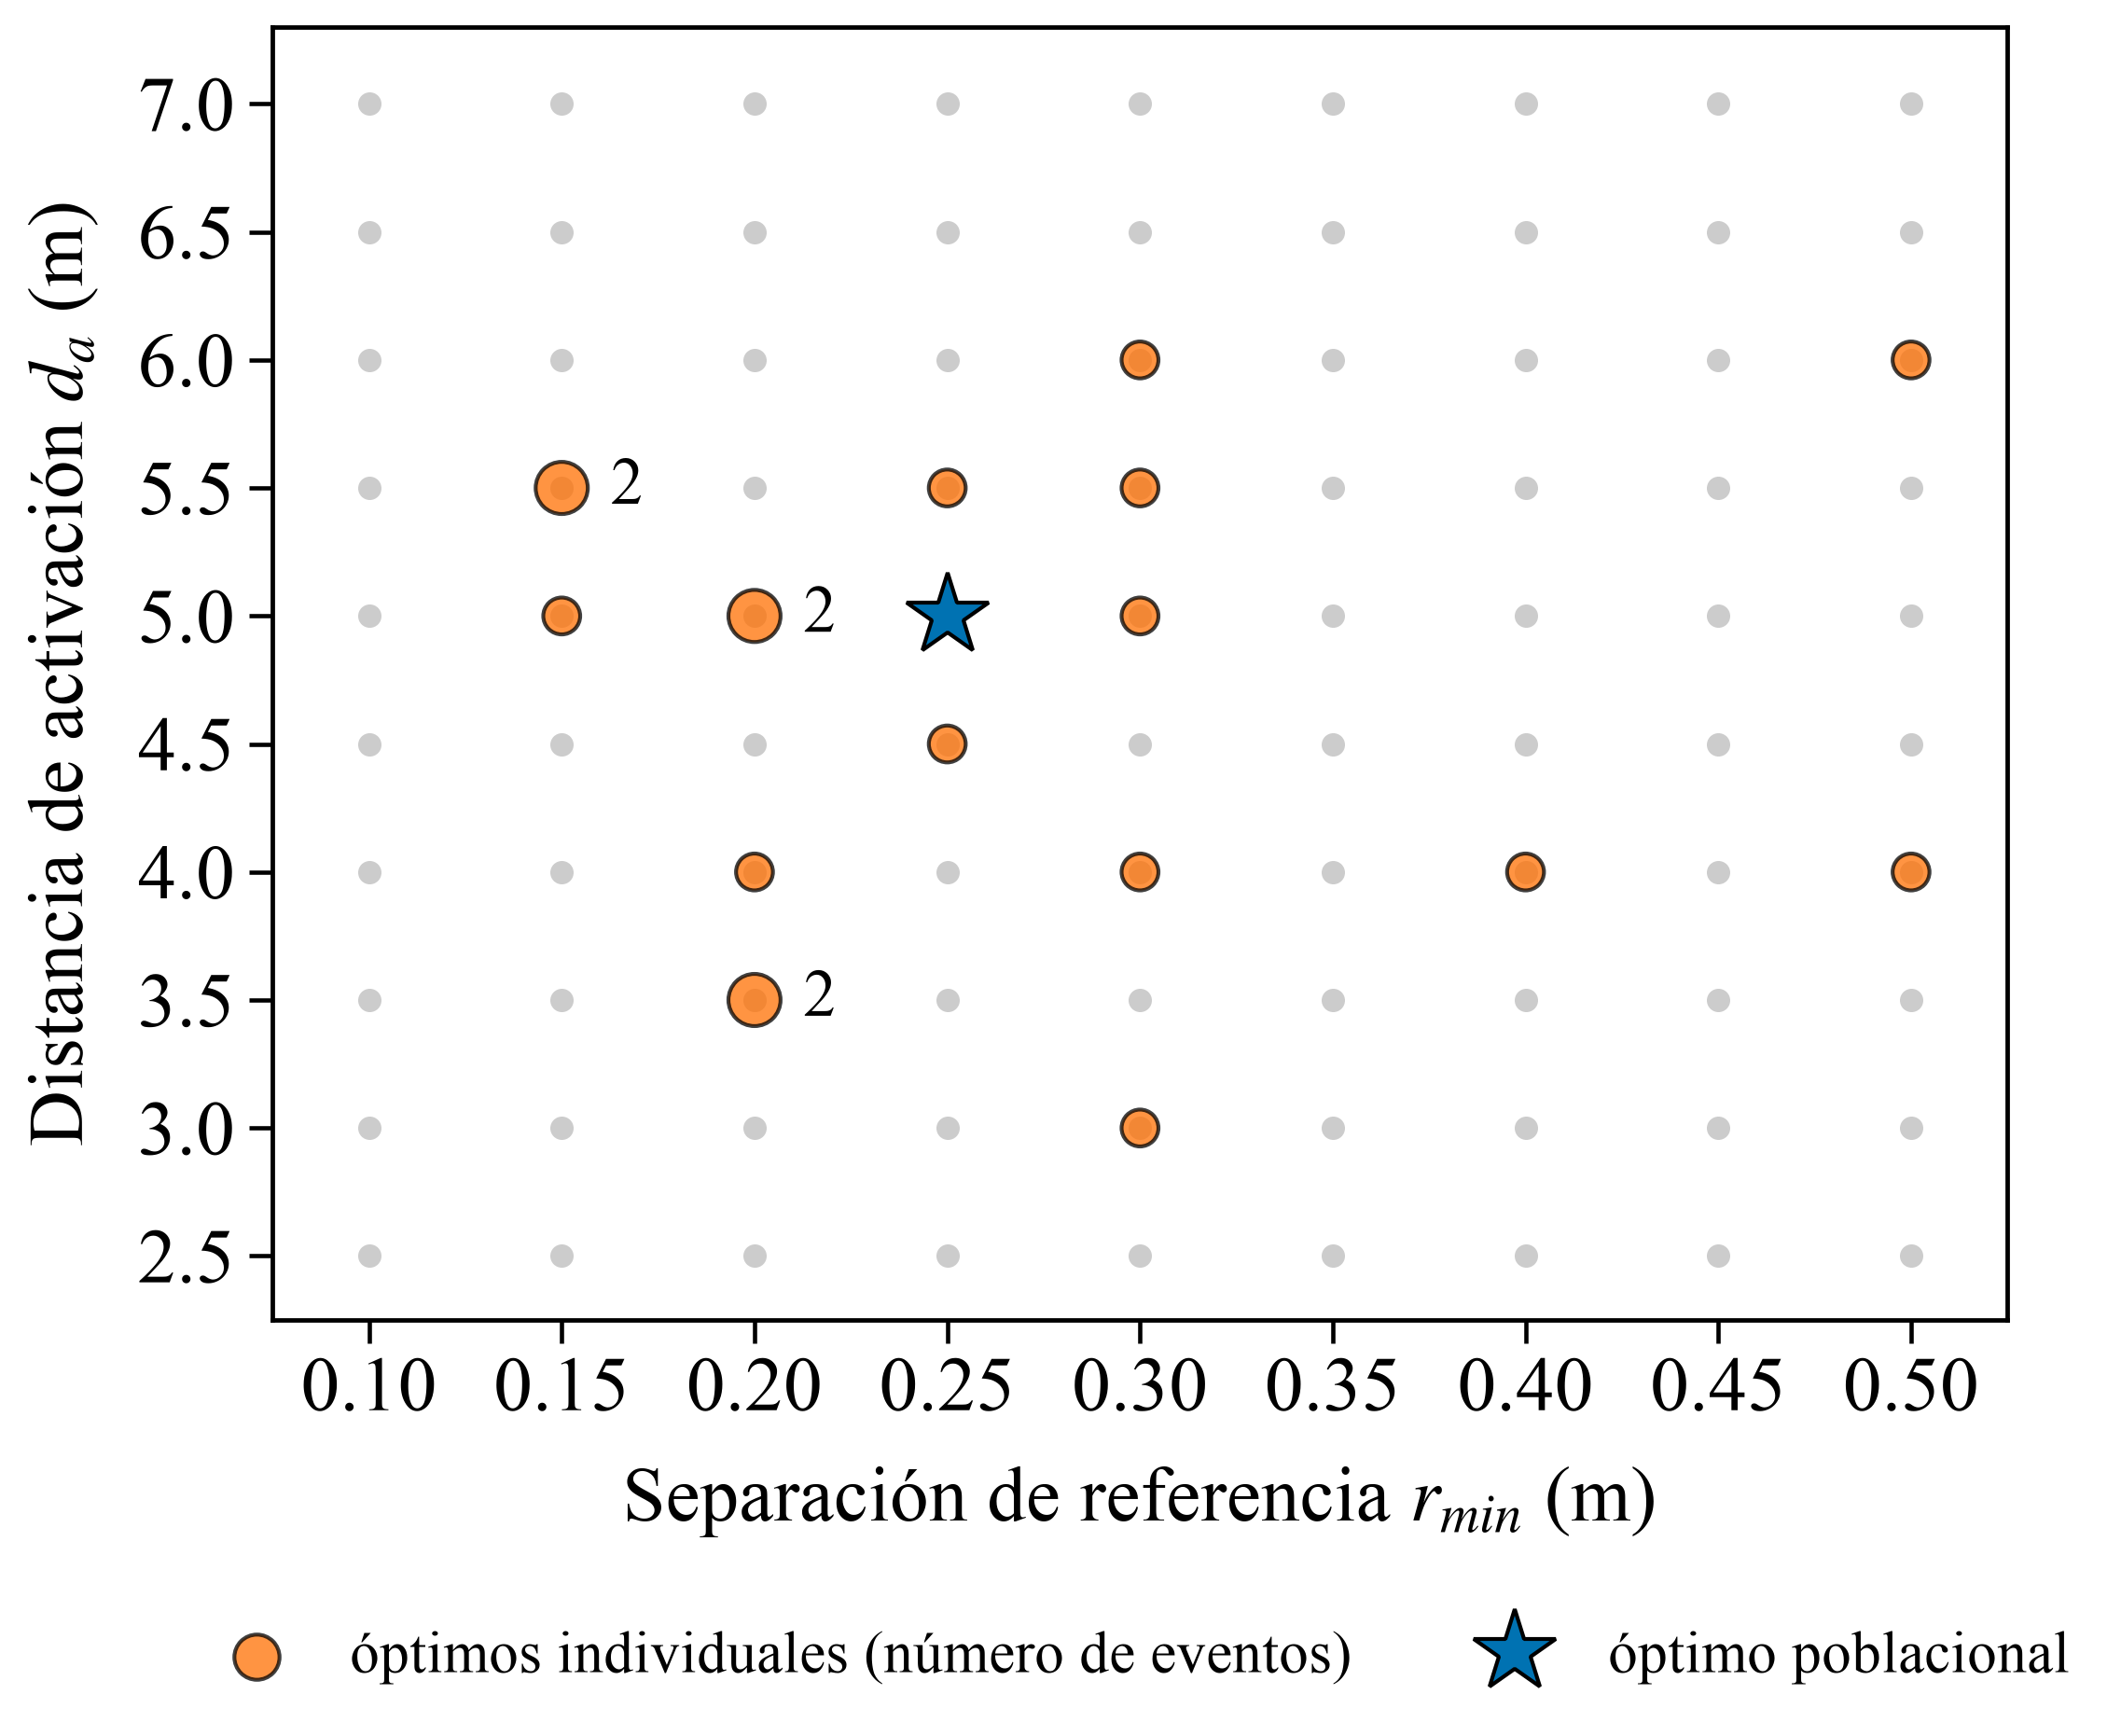
\includegraphics[width=\linewidth,height=0.70\textheight,keepaspectratio]{E2_optimos_individuales.png}
    \end{column}
  \end{columns}
\end{frame}

\begin{frame}{Resultados}
  \framesubtitle{Calibración individual: error de cada evento}
  \begin{columns}[T]
    \begin{column}{0.49\textwidth}
      \centering{\small Métrica 1}\par
      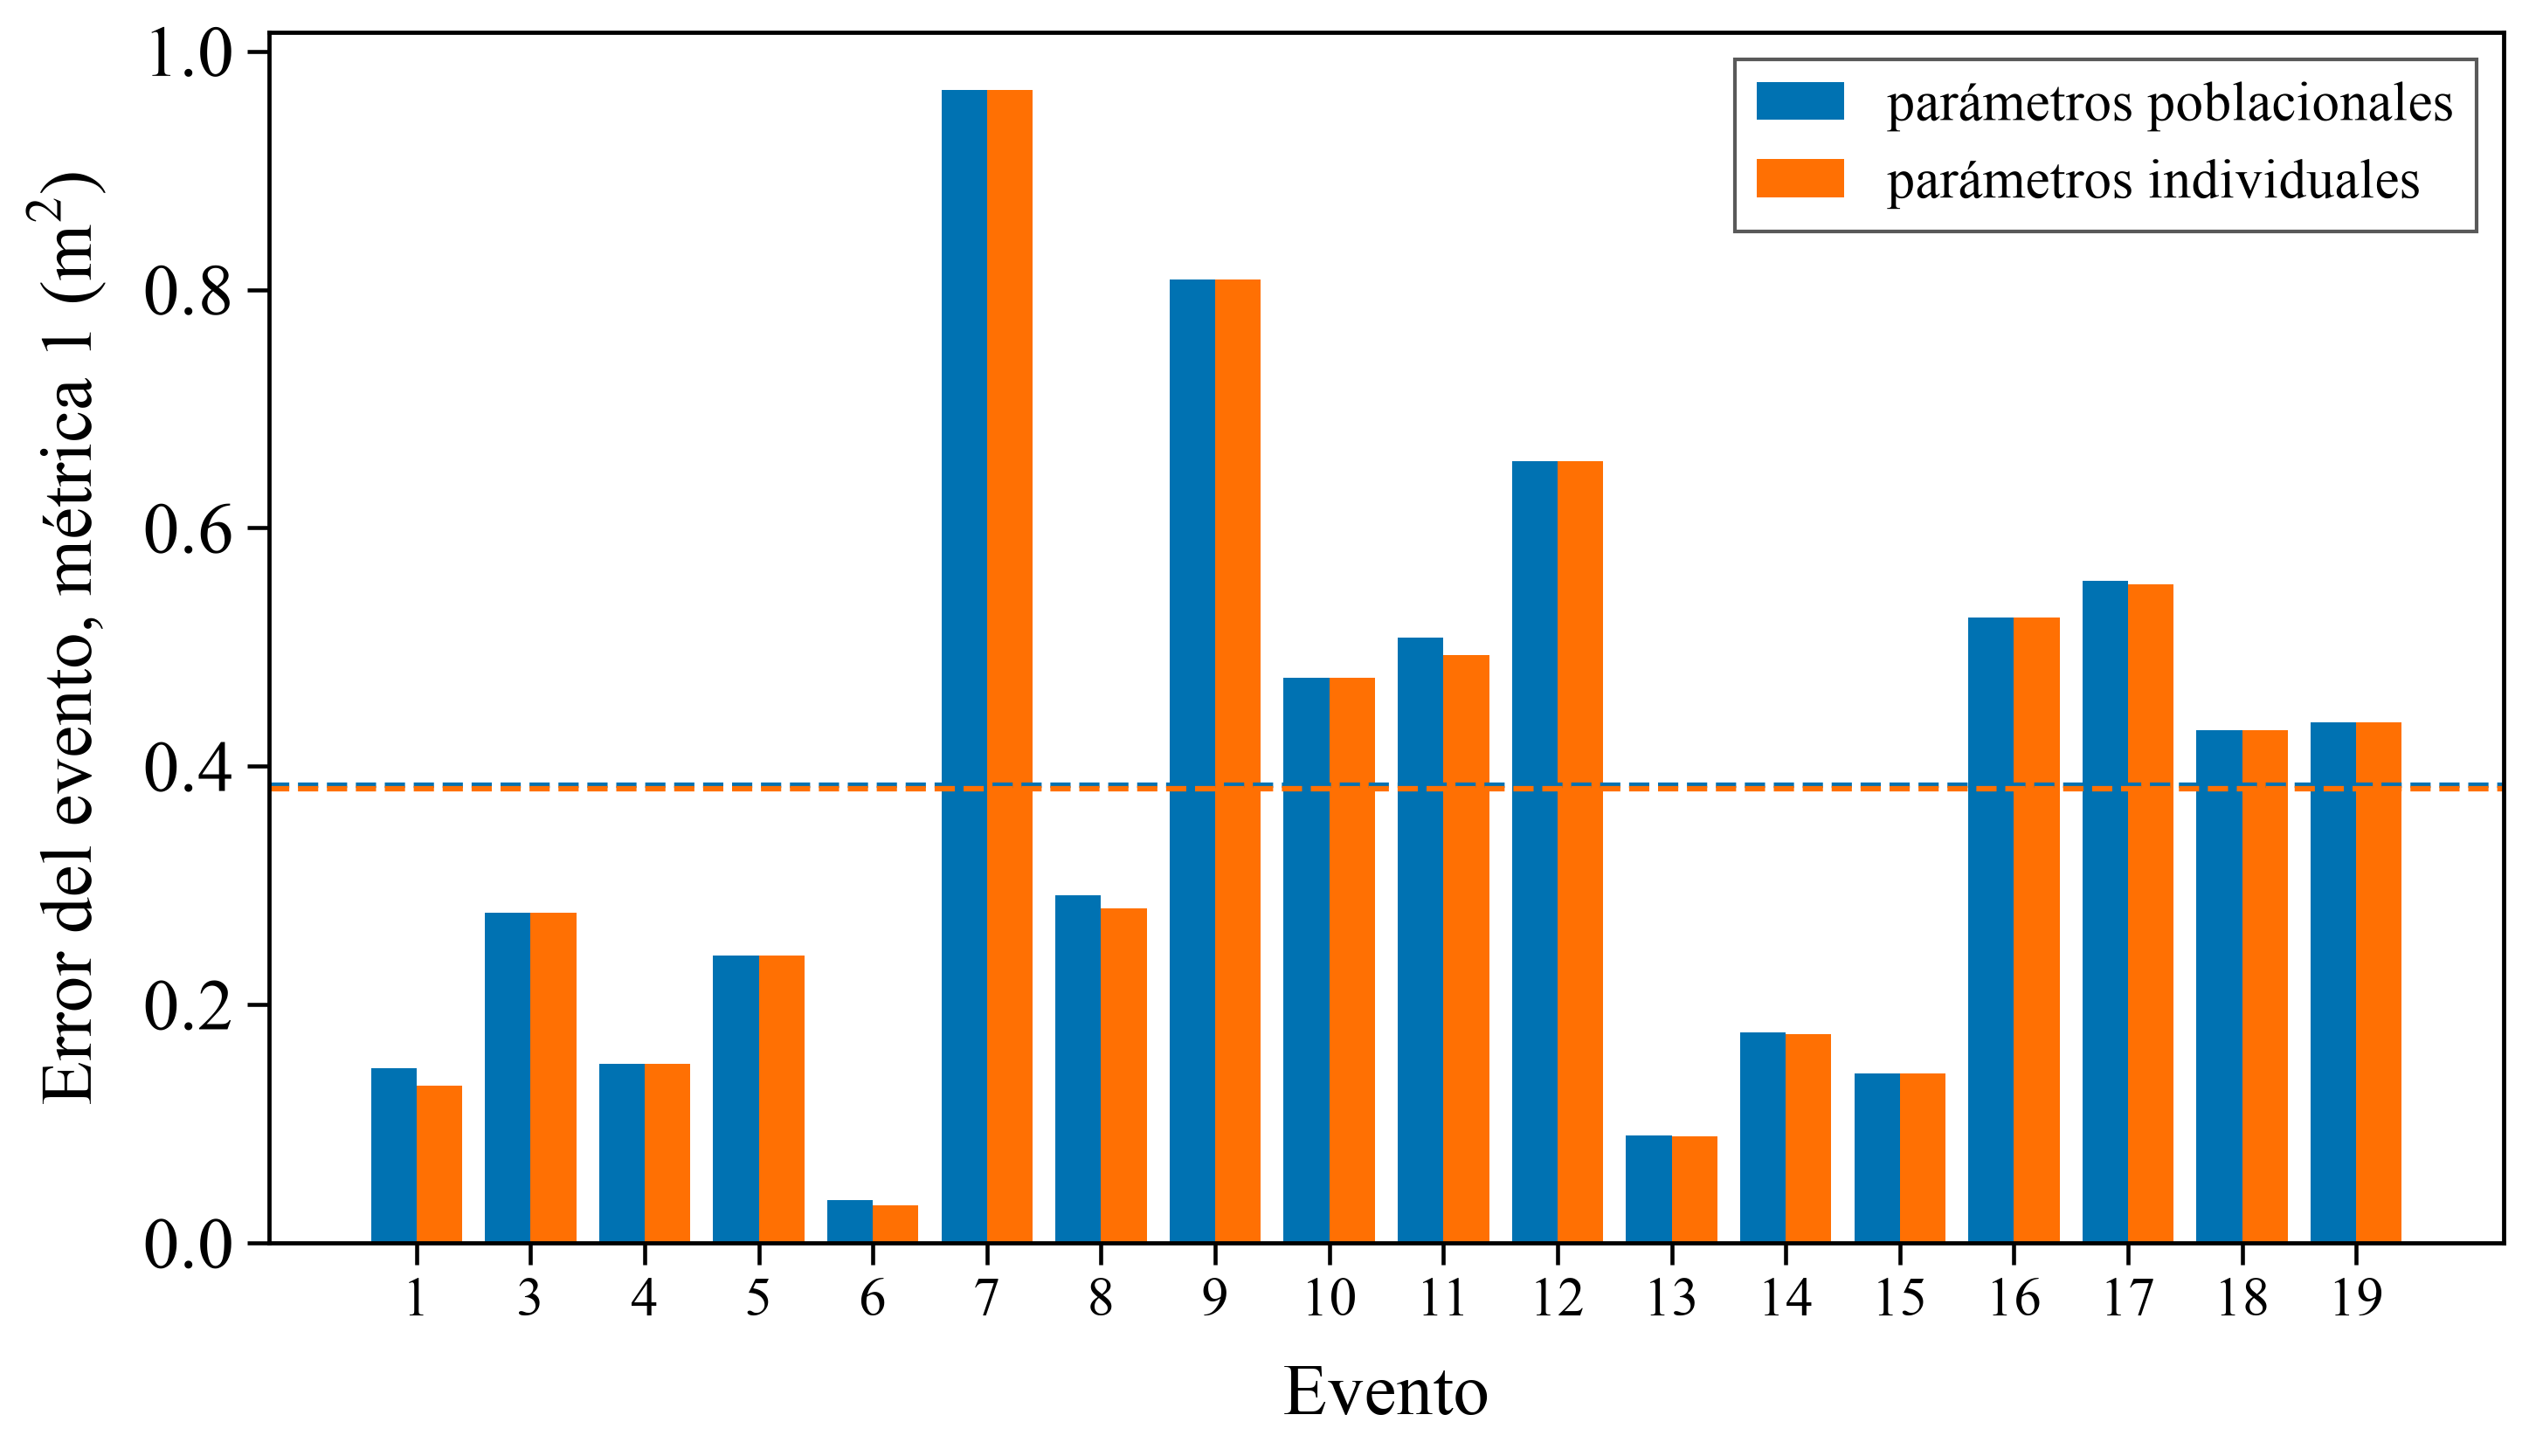
\includegraphics[width=\linewidth,height=0.70\textheight,keepaspectratio]{E1_error_por_evento.png}
    \end{column}
    \begin{column}{0.49\textwidth}
      \centering{\small Métrica 2}\par
      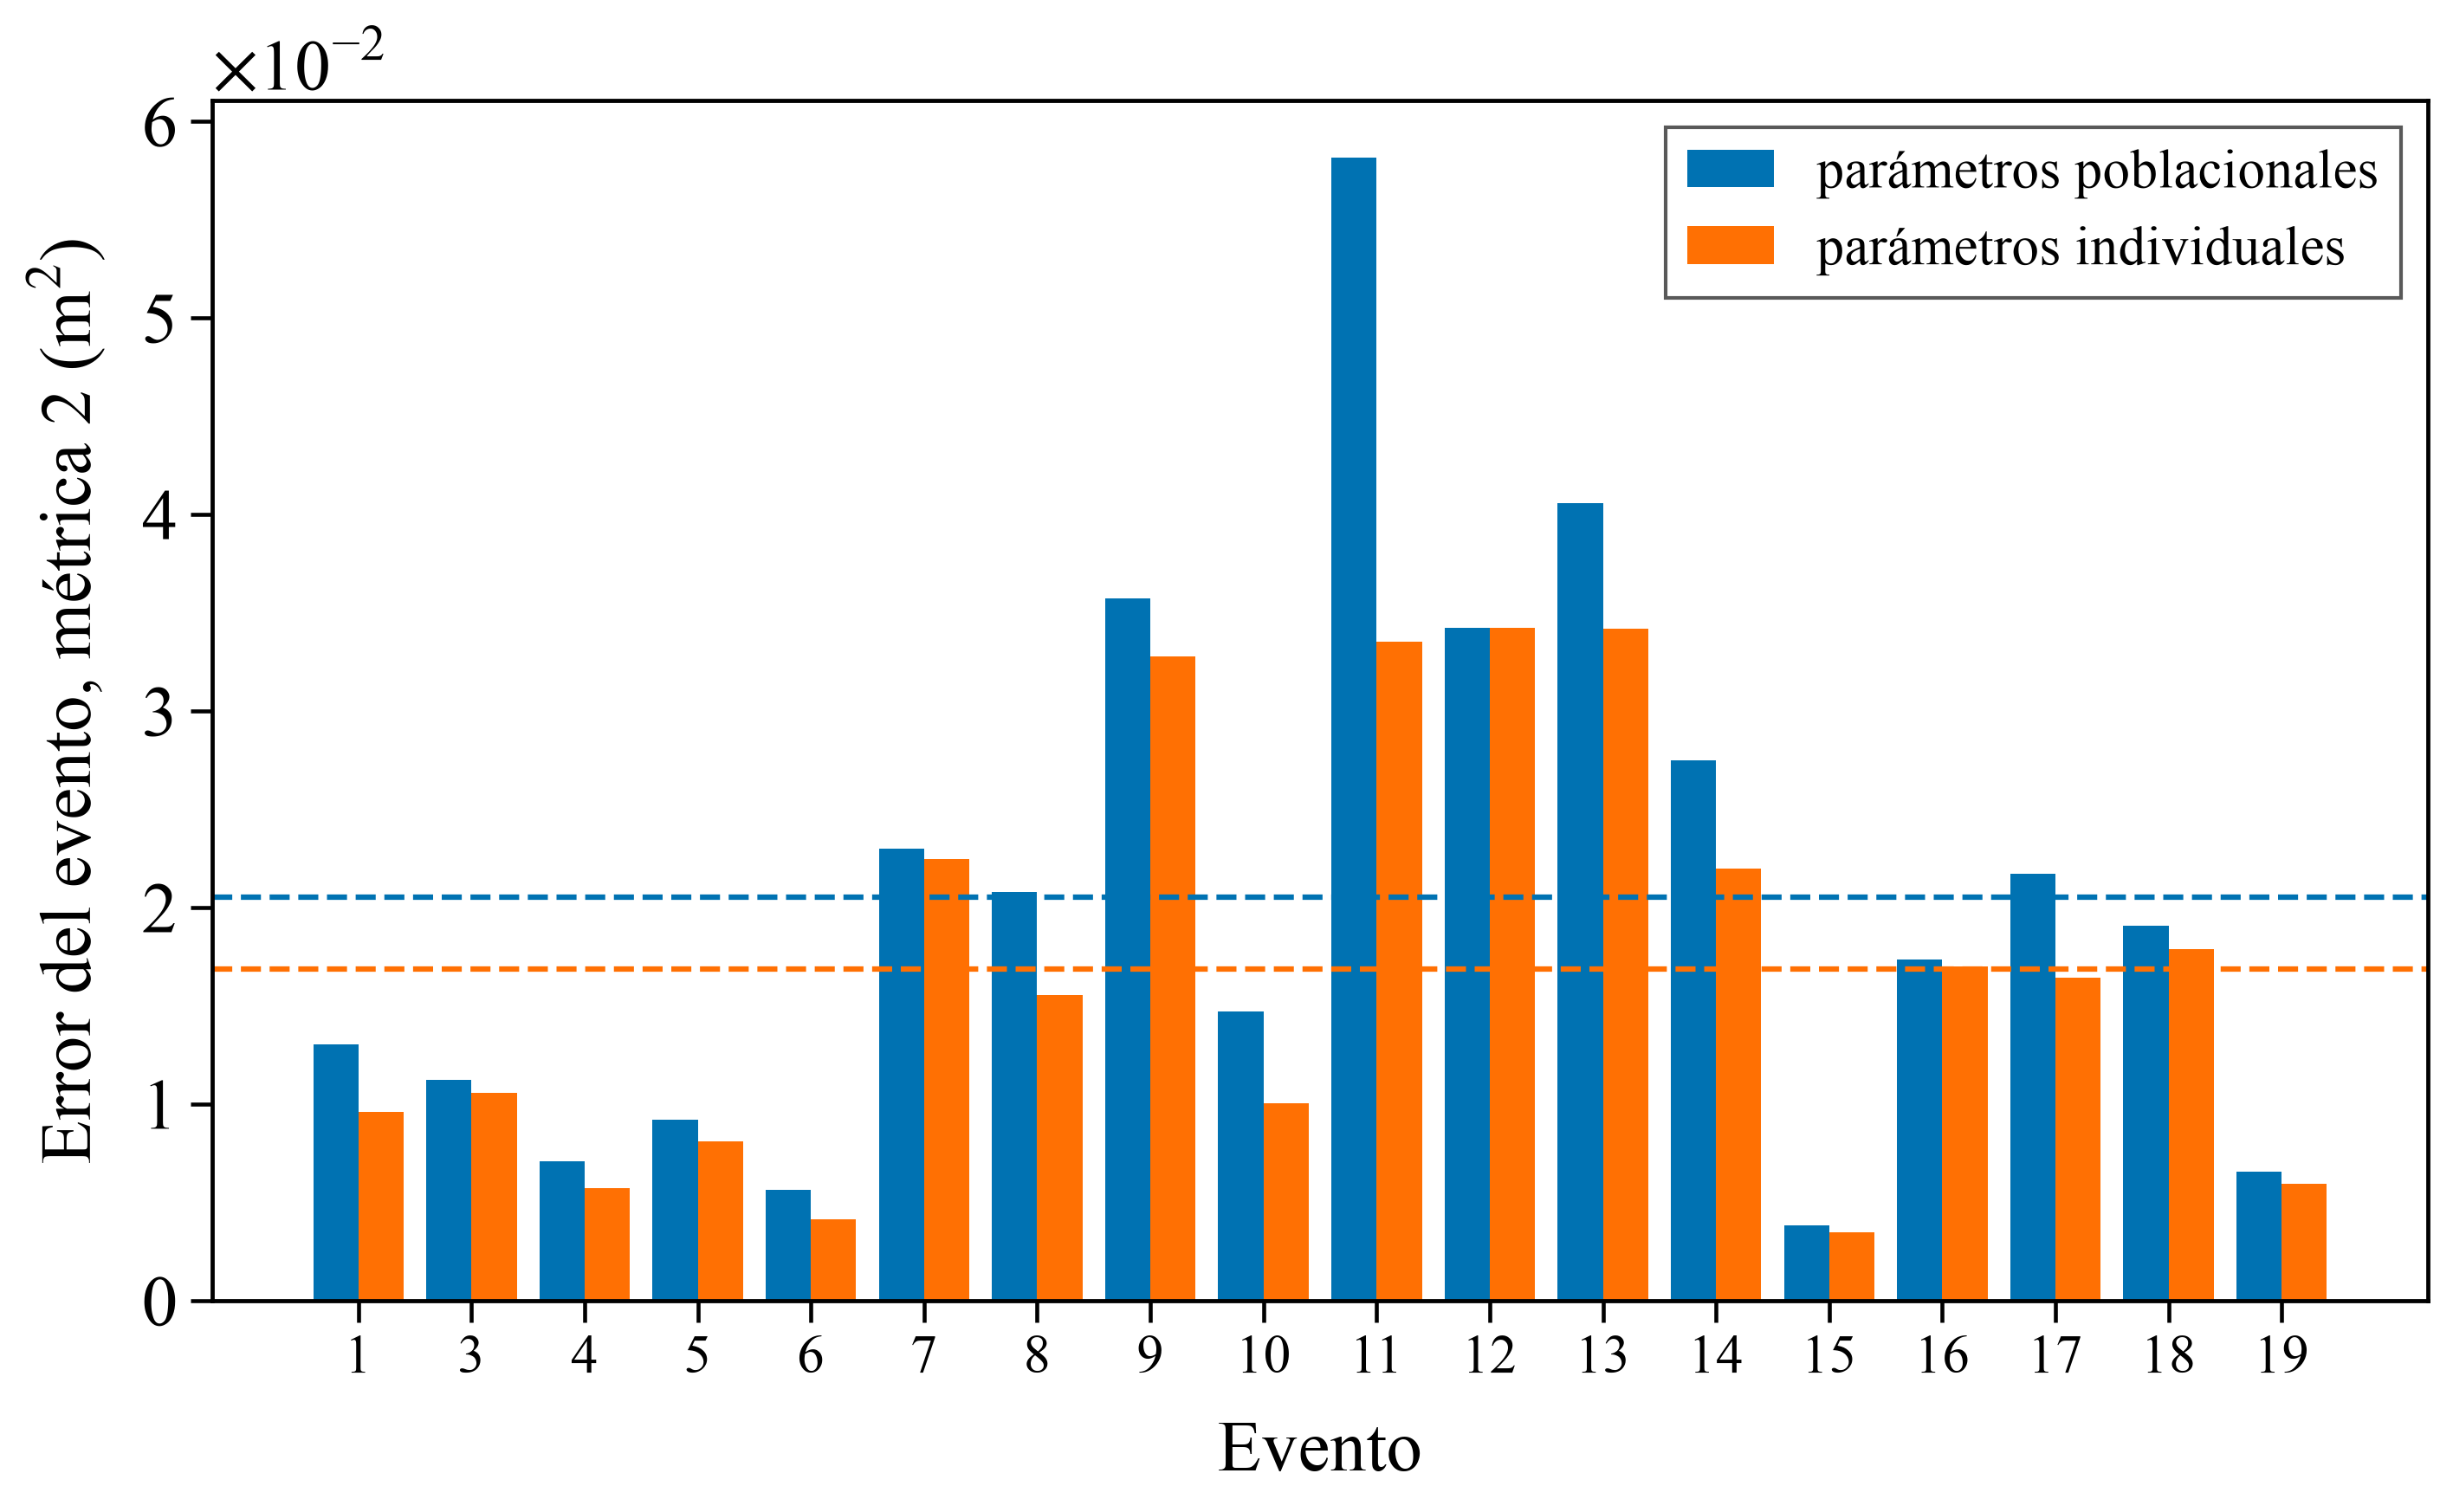
\includegraphics[width=\linewidth,height=0.70\textheight,keepaspectratio]{E2_error_por_evento.png}
    \end{column}
  \end{columns}
\end{frame}

\begin{frame}{Resultados}
  \framesubtitle{Calibración individual: ganancia al individualizar}
  \centering
  \renewcommand{\arraystretch}{1.5}
  \begin{tabular}{lccc}
    \hline
    Métrica & $\langle E\rangle$ poblacional (m$^2$) & $\langle E\rangle$ individual (m$^2$) & Ganancia \\
    \hline
    1: iguales tiempos & $0.384$ & $0.381$ & $0.7$\,\% \\
    2: punto más cercano & $2.05\ten{-2}$ & $1.69\ten{-2}$ & $18$\,\% \\
    \hline
  \end{tabular}

  \vspace{16pt}
  \begin{columns}
    \begin{column}{0.62\textwidth}
      \begin{resultado}
        \item Ganancia $= \big(\langle E\rangle_{\mathrm{pob}} - \langle E\rangle_{\mathrm{ind}}\big) / \langle E\rangle_{\mathrm{pob}}$
        \item $\sqrt{\langle E\rangle}$, métrica 1: $0.620 \to 0.618\uni{m}$
        \item $\sqrt{\langle E\rangle}$, métrica 2: $0.143 \to 0.130\uni{m}$
      \end{resultado}
    \end{column}
  \end{columns}
\end{frame}

\begin{frame}{Resultados}
  \framesubtitle{Validación cruzada}
\end{frame}


\section{Conclusiones}
\begin{frame}{Conclusiones}
  \begin{itemize}\setlength{\itemsep}{14pt}
    \item Missing
    \item Missing
    \item Missing
  \end{itemize}
\end{frame}


\begin{frame}[plain,noframenumbering]
  \vfill\centering{\Huge\usebeamercolor[fg]{structure}Muchas gracias}\vfill
\end{frame}

\begin{frame}{Declaración de uso de IA}
  \begin{itemize}\setlength{\itemsep}{10pt}
    \item Agente: Claude Code
    \item Modelo: Claude Opus 5.5
    \item Uso:
      \begin{itemize}
        \item Elaboración de los scripts de postprocesamiento
        \item Correcciones de código
        \item Evaluación de presentación según rúbrica de cátedra
      \end{itemize}
  \end{itemize}
\end{frame}


\appendix
\section*{Anexo}
\begin{frame}[plain,noframenumbering]
\vfill\centering{\Huge\usebeamercolor[fg]{structure}Anexo}\vfill
\end{frame}
\begin{frame}{Anexo}
  \framesubtitle{Capa de elusión: geometría completa}
  \large
  Marco local de $i$, con $\hat{\vv{u}}$ hacia el target final y $\hat{\vv{n}} = (u_y,\,-u_x)$:
  \[
    s = (\vv{r}_j - \vv{r}_i)\cdot\hat{\vv{u}}, \qquad \ell = (\vv{r}_j - \vv{r}_i)\cdot\hat{\vv{n}}
  \]
  \vspace{2pt}
  Parábola por $i$, punto de paso $P = (s,\ \ell + R)$ y target final:
  \[
    y(x) = (\ell + R)\,\frac{x\,(D - x)}{s\,(D - s)}
    \qquad\Rightarrow\qquad
    y'(0) = \frac{(\ell + R)\,D}{s\,(D - s)}
  \]
  \vspace{2pt}
  Target temporal, sobre tangente a parábola en $i$:
  \[
    \vv{x}^{\,temp}_i = \vv{r}_i + s\,\hat{\vv{u}} + s\,y'(0)\,\hat{\vv{n}},
    \qquad
    \vv{e}_0 = \frac{\vv{x}^{\,temp}_i - \vv{r}_i}{|\vv{x}^{\,temp}_i - \vv{r}_i|}
  \]
\end{frame}

\begin{frame}{Anexo}
  \framesubtitle{Validación cruzada: valores de error medio}
  \centering
  \renewcommand{\arraystretch}{1.5}
  \begin{tabular}{lccc}
    \hline
    Métrica & Poblacional (m$^2$) & Entrenamiento (m$^2$) & Validación (m$^2$) \\
    \hline
    1: iguales tiempos & $0.384$ & $0.39 \pm 0.04$ & $0.4 \pm 0.1$ \\
    2: punto más cercano & $2.05\ten{-2}$ & $(2.0 \pm 0.2)\ten{-2}$ & $(2.1 \pm 0.6)\ten{-2}$ \\
    \hline
  \end{tabular}

  \vspace{16pt}
  \begin{columns}
    \begin{column}{0.62\textwidth}
      \begin{parametros}
        \item 20 particiones aleatorias: 13 eventos de entrenamiento, 5 de validación
      \end{parametros}
    \end{column}
  \end{columns}
\end{frame}


\end{document}
